\section{Comparison of Importance Sampling method}
\label{sec:simulation_studies}

We now have three tools to produce Gaussian importance sampling proposals: the \gls{la}, the \gls{cem} and \gls{eis}. Naturally, we want to choose the optimal tool for the problem at hand. In this section, we investigate under which circumstances which method is to be preferred over the others. To judge the performance of each method, we will discuss the following quality criteria:
\begin{itemize}
    % speed of convergence, i.e. asymptotic variance
    % performance at the optimum
    % computation time - though not hard, only theoretical
    % numerical stability (?)
    \item breakdown of methods,
    \item time and space complexity of the method,
    \item speed of stochastic convergence, as indicated by the asymptotic variance, for the \gls{cem} and \gls{eis},
    \item speed of numerical convergence, as indicated by the number of iterations until \Cref{alg:cem-markov-proposal-fast,alg:eis} reach numerical convergence for fixed sample size $N$ and precision $\epsilon$, and
    \item performance of the optimal proposal, as measured by the efficiency factor, especially as $n$ or $m$ comes larger. 
\end{itemize}
Let us elaborate on these criteria. With a breakdown of the methods, we mean settings in which either the numerical scheme diverges, produces parameters that lead to invalid proposals, i.e. negative variances, or where the proposals fail to produce consistent importance sampling estimates. 
Time and space complexity allow us to compare the methods theoretically, i.e. be independent of implementation details. The speed of stochastic convergence is relevant as well: The smaller the asymptotic variance, the smaller we can choose the sample size $N$ and thus decrease computation time. Similarly, numerical convergence directly affects computation time. \todo{reformulate this paragraph nicer} Finally, if one method has vastly better performance at the optimum, we might be willing to spend more time initially to save time later when we use the proposal to perform inference. Of special interest is the performance for long (large $n$) or fat (large $m$) time series, as the models we fit in \Cref{cha:analysis_of_selected_models} usually fall into one of these categories.

\subsection{Breakdown of methods}

Let us start with a classical example in which the \gls{la} fails to produce consistent importance sampling estimates. 
\begin{example}[Failure of \gls{la}]
  \label{ex:la_failure}
  Consider the Gaussian scale mixture $\P = \frac{1}{2} \left(\mathcal N (0,1) + \mathcal N(0, \varepsilon^{-2})\right)$ with mode $x^{\ast}=0$. 
  The \gls{la} is $\G_{\text{LA}} = \mathcal N \left( 0, \frac{1}{\varepsilon^{2} - \varepsilon + 1} \right)$, whose variance goes to $1$ as $\varepsilon$ goes to $0$, so the \gls{la} will miss close to $\frac 1 2$ of the total mass.
  For $\varepsilon$ small enough, the variance of the \gls{la} will be smaller than $\frac{1}{2\varepsilon^{2}}$, whence the second moment of the weights is infinite and importance sampling with $\G_{\text{LA}}$ is inconsistent.

  The \gls{cem} minimizes the KL-divergence between $\P$ and $\G_{\psi}$, is given by $\G_{\text{CE}} = \mathcal N (0, \sigma^{2})$, where $\sigma^{2} = \frac{1}{2}\left( 1 + \varepsilon^{-2} \right)$ is the variance of $\P$.
  As $\sigma^{2} > \frac{1}{2}\varepsilon^{-2}$, the weights have finite second moment, and importance sampling with $\G_{\ce}$ is consistent.
  \todo{add proof for $\frac{1}{2}$ to appendix}

  As \Gls{eis} does not yield analytically tractable proposals in this setting, we resort to a simulation study. Using the same setup as described in \Cref{ex:univ-gaussian-s2-fixed}, we replicate $M = 100$ times $\hpce$ and $\hpeis$ for varying levels of $\varepsilon^{2}$. The resulting excess variances, i.e. $\sigma^{2} - \left( \frac{1}{2} + \frac{1}{2 \varepsilon^{2}} \right)$, efficiency factors and asymptotic efficiencies are displayed in \Cref{fig:gsmm_eps}. We see that for small $\varepsilon^{2}$, \aeis is inconsistent, while the \acem stays consistent. However, as is to be expected, for small $\varepsilon^{2}$, the efficiency factor becomes very small.
    \begin{figure}
        \centering

        \resizebox{\textwidth}{!}{%
            % Created by tikzDevice version 0.12.6 on 2024-06-10 16:58:27
% !TEX encoding = UTF-8 Unicode
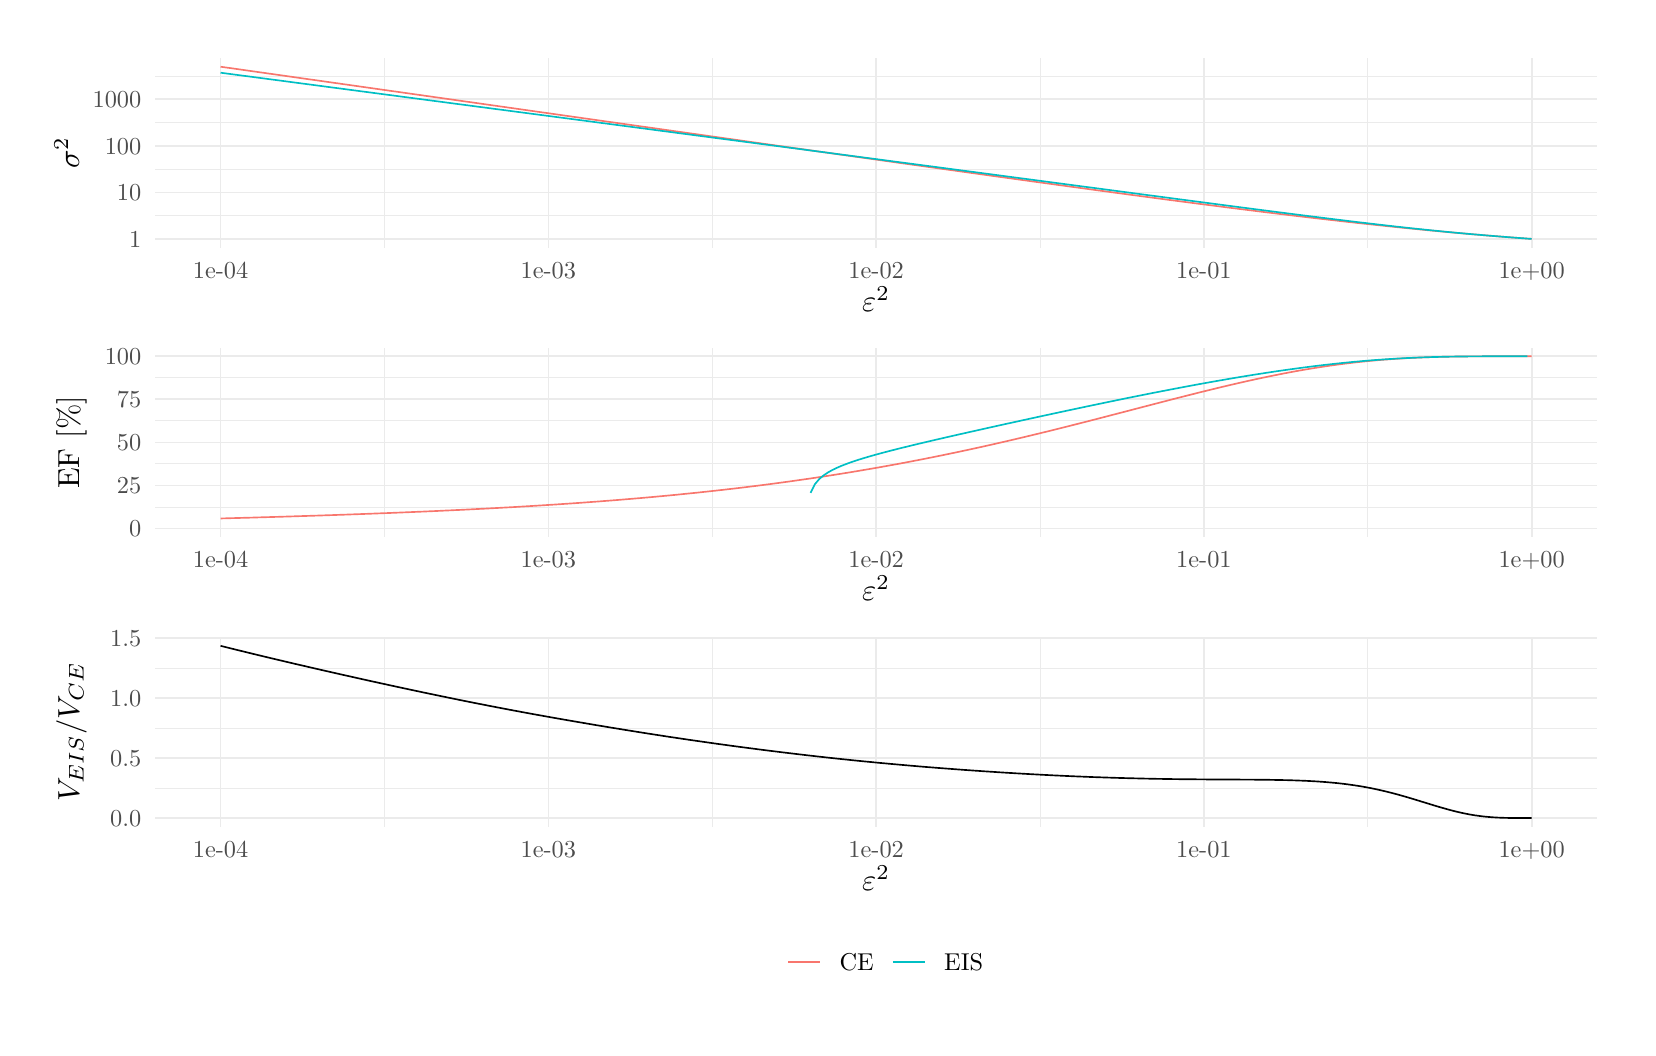
\begin{tikzpicture}[x=1pt,y=1pt]
\definecolor{fillColor}{RGB}{255,255,255}
\path[use as bounding box,fill=fillColor,fill opacity=0.00] (0,0) rectangle (578.16,361.35);
\begin{scope}
\path[clip] ( 46.01,281.90) rectangle (567.16,350.35);
\definecolor{drawColor}{gray}{0.92}

\path[draw=drawColor,line width= 0.3pt,line join=round] ( 46.01,293.43) --
	(567.16,293.43);

\path[draw=drawColor,line width= 0.3pt,line join=round] ( 46.01,310.25) --
	(567.16,310.25);

\path[draw=drawColor,line width= 0.3pt,line join=round] ( 46.01,327.07) --
	(567.16,327.07);

\path[draw=drawColor,line width= 0.3pt,line join=round] ( 46.01,343.89) --
	(567.16,343.89);

\path[draw=drawColor,line width= 0.3pt,line join=round] (128.92,281.90) --
	(128.92,350.35);

\path[draw=drawColor,line width= 0.3pt,line join=round] (247.36,281.90) --
	(247.36,350.35);

\path[draw=drawColor,line width= 0.3pt,line join=round] (365.81,281.90) --
	(365.81,350.35);

\path[draw=drawColor,line width= 0.3pt,line join=round] (484.25,281.90) --
	(484.25,350.35);

\path[draw=drawColor,line width= 0.6pt,line join=round] ( 46.01,285.02) --
	(567.16,285.02);

\path[draw=drawColor,line width= 0.6pt,line join=round] ( 46.01,301.84) --
	(567.16,301.84);

\path[draw=drawColor,line width= 0.6pt,line join=round] ( 46.01,318.66) --
	(567.16,318.66);

\path[draw=drawColor,line width= 0.6pt,line join=round] ( 46.01,335.48) --
	(567.16,335.48);

\path[draw=drawColor,line width= 0.6pt,line join=round] ( 69.70,281.90) --
	( 69.70,350.35);

\path[draw=drawColor,line width= 0.6pt,line join=round] (188.14,281.90) --
	(188.14,350.35);

\path[draw=drawColor,line width= 0.6pt,line join=round] (306.59,281.90) --
	(306.59,350.35);

\path[draw=drawColor,line width= 0.6pt,line join=round] (425.03,281.90) --
	(425.03,350.35);

\path[draw=drawColor,line width= 0.6pt,line join=round] (543.47,281.90) --
	(543.47,350.35);
\definecolor{drawColor}{RGB}{248,118,109}

\path[draw=drawColor,line width= 0.6pt,line join=round] ( 69.70,347.24) --
	( 71.28,347.01) --
	( 72.86,346.79) --
	( 74.44,346.57) --
	( 76.02,346.34) --
	( 77.59,346.12) --
	( 79.17,345.89) --
	( 80.75,345.67) --
	( 82.33,345.45) --
	( 83.91,345.22) --
	( 85.49,345.00) --
	( 87.07,344.77) --
	( 88.65,344.55) --
	( 90.23,344.32) --
	( 91.81,344.10) --
	( 93.39,343.88) --
	( 94.97,343.65) --
	( 96.55,343.43) --
	( 98.13,343.20) --
	( 99.70,342.98) --
	(101.28,342.75) --
	(102.86,342.53) --
	(104.44,342.31) --
	(106.02,342.08) --
	(107.60,341.86) --
	(109.18,341.63) --
	(110.76,341.41) --
	(112.34,341.19) --
	(113.92,340.96) --
	(115.50,340.74) --
	(117.08,340.51) --
	(118.66,340.29) --
	(120.23,340.06) --
	(121.81,339.84) --
	(123.39,339.62) --
	(124.97,339.39) --
	(126.55,339.17) --
	(128.13,338.94) --
	(129.71,338.72) --
	(131.29,338.49) --
	(132.87,338.27) --
	(134.45,338.05) --
	(136.03,337.82) --
	(137.61,337.60) --
	(139.19,337.37) --
	(140.76,337.15) --
	(142.34,336.93) --
	(143.92,336.70) --
	(145.50,336.48) --
	(147.08,336.25) --
	(148.66,336.03) --
	(150.24,335.80) --
	(151.82,335.58) --
	(153.40,335.36) --
	(154.98,335.13) --
	(156.56,334.91) --
	(158.14,334.68) --
	(159.72,334.46) --
	(161.29,334.24) --
	(162.87,334.01) --
	(164.45,333.79) --
	(166.03,333.56) --
	(167.61,333.34) --
	(169.19,333.12) --
	(170.77,332.89) --
	(172.35,332.67) --
	(173.93,332.44) --
	(175.51,332.22) --
	(177.09,331.99) --
	(178.67,331.77) --
	(180.25,331.55) --
	(181.82,331.32) --
	(183.40,331.10) --
	(184.98,330.87) --
	(186.56,330.65) --
	(188.14,330.43) --
	(189.72,330.20) --
	(191.30,329.98) --
	(192.88,329.75) --
	(194.46,329.53) --
	(196.04,329.31) --
	(197.62,329.08) --
	(199.20,328.86) --
	(200.78,328.63) --
	(202.36,328.41) --
	(203.93,328.19) --
	(205.51,327.96) --
	(207.09,327.74) --
	(208.67,327.51) --
	(210.25,327.29) --
	(211.83,327.07) --
	(213.41,326.84) --
	(214.99,326.62) --
	(216.57,326.40) --
	(218.15,326.17) --
	(219.73,325.95) --
	(221.31,325.72) --
	(222.89,325.50) --
	(224.46,325.28) --
	(226.04,325.05) --
	(227.62,324.83) --
	(229.20,324.60) --
	(230.78,324.38) --
	(232.36,324.16) --
	(233.94,323.93) --
	(235.52,323.71) --
	(237.10,323.49) --
	(238.68,323.26) --
	(240.26,323.04) --
	(241.84,322.82) --
	(243.42,322.59) --
	(244.99,322.37) --
	(246.57,322.14) --
	(248.15,321.92) --
	(249.73,321.70) --
	(251.31,321.47) --
	(252.89,321.25) --
	(254.47,321.03) --
	(256.05,320.80) --
	(257.63,320.58) --
	(259.21,320.36) --
	(260.79,320.13) --
	(262.37,319.91) --
	(263.95,319.69) --
	(265.52,319.46) --
	(267.10,319.24) --
	(268.68,319.02) --
	(270.26,318.79) --
	(271.84,318.57) --
	(273.42,318.35) --
	(275.00,318.12) --
	(276.58,317.90) --
	(278.16,317.68) --
	(279.74,317.46) --
	(281.32,317.23) --
	(282.90,317.01) --
	(284.48,316.79) --
	(286.05,316.56) --
	(287.63,316.34) --
	(289.21,316.12) --
	(290.79,315.90) --
	(292.37,315.67) --
	(293.95,315.45) --
	(295.53,315.23) --
	(297.11,315.01) --
	(298.69,314.78) --
	(300.27,314.56) --
	(301.85,314.34) --
	(303.43,314.12) --
	(305.01,313.90) --
	(306.59,313.67) --
	(308.16,313.45) --
	(309.74,313.23) --
	(311.32,313.01) --
	(312.90,312.79) --
	(314.48,312.56) --
	(316.06,312.34) --
	(317.64,312.12) --
	(319.22,311.90) --
	(320.80,311.68) --
	(322.38,311.46) --
	(323.96,311.24) --
	(325.54,311.01) --
	(327.12,310.79) --
	(328.69,310.57) --
	(330.27,310.35) --
	(331.85,310.13) --
	(333.43,309.91) --
	(335.01,309.69) --
	(336.59,309.47) --
	(338.17,309.25) --
	(339.75,309.03) --
	(341.33,308.81) --
	(342.91,308.59) --
	(344.49,308.37) --
	(346.07,308.15) --
	(347.65,307.93) --
	(349.22,307.71) --
	(350.80,307.49) --
	(352.38,307.27) --
	(353.96,307.05) --
	(355.54,306.84) --
	(357.12,306.62) --
	(358.70,306.40) --
	(360.28,306.18) --
	(361.86,305.96) --
	(363.44,305.74) --
	(365.02,305.53) --
	(366.60,305.31) --
	(368.18,305.09) --
	(369.75,304.88) --
	(371.33,304.66) --
	(372.91,304.44) --
	(374.49,304.23) --
	(376.07,304.01) --
	(377.65,303.79) --
	(379.23,303.58) --
	(380.81,303.36) --
	(382.39,303.15) --
	(383.97,302.93) --
	(385.55,302.72) --
	(387.13,302.50) --
	(388.71,302.29) --
	(390.28,302.08) --
	(391.86,301.86) --
	(393.44,301.65) --
	(395.02,301.44) --
	(396.60,301.23) --
	(398.18,301.01) --
	(399.76,300.80) --
	(401.34,300.59) --
	(402.92,300.38) --
	(404.50,300.17) --
	(406.08,299.96) --
	(407.66,299.75) --
	(409.24,299.54) --
	(410.82,299.33) --
	(412.39,299.12) --
	(413.97,298.92) --
	(415.55,298.71) --
	(417.13,298.50) --
	(418.71,298.30) --
	(420.29,298.09) --
	(421.87,297.88) --
	(423.45,297.68) --
	(425.03,297.48) --
	(426.61,297.27) --
	(428.19,297.07) --
	(429.77,296.87) --
	(431.35,296.67) --
	(432.92,296.46) --
	(434.50,296.26) --
	(436.08,296.06) --
	(437.66,295.86) --
	(439.24,295.67) --
	(440.82,295.47) --
	(442.40,295.27) --
	(443.98,295.07) --
	(445.56,294.88) --
	(447.14,294.68) --
	(448.72,294.49) --
	(450.30,294.30) --
	(451.88,294.10) --
	(453.45,293.91) --
	(455.03,293.72) --
	(456.61,293.53) --
	(458.19,293.34) --
	(459.77,293.16) --
	(461.35,292.97) --
	(462.93,292.78) --
	(464.51,292.60) --
	(466.09,292.41) --
	(467.67,292.23) --
	(469.25,292.05) --
	(470.83,291.87) --
	(472.41,291.69) --
	(473.98,291.51) --
	(475.56,291.33) --
	(477.14,291.15) --
	(478.72,290.98) --
	(480.30,290.80) --
	(481.88,290.63) --
	(483.46,290.46) --
	(485.04,290.29) --
	(486.62,290.12) --
	(488.20,289.95) --
	(489.78,289.79) --
	(491.36,289.62) --
	(492.94,289.46) --
	(494.51,289.29) --
	(496.09,289.13) --
	(497.67,288.97) --
	(499.25,288.81) --
	(500.83,288.66) --
	(502.41,288.50) --
	(503.99,288.35) --
	(505.57,288.19) --
	(507.15,288.04) --
	(508.73,287.89) --
	(510.31,287.75) --
	(511.89,287.60) --
	(513.47,287.45) --
	(515.05,287.31) --
	(516.62,287.17) --
	(518.20,287.03) --
	(519.78,286.89) --
	(521.36,286.75) --
	(522.94,286.62) --
	(524.52,286.49) --
	(526.10,286.35) --
	(527.68,286.22) --
	(529.26,286.10) --
	(530.84,285.97) --
	(532.42,285.84) --
	(534.00,285.72) --
	(535.58,285.60) --
	(537.15,285.48) --
	(538.73,285.36) --
	(540.31,285.24) --
	(541.89,285.13) --
	(543.47,285.02);
\definecolor{drawColor}{RGB}{0,191,196}

\path[draw=drawColor,line width= 0.6pt,line join=round] ( 69.70,345.07) --
	( 71.28,344.86) --
	( 72.86,344.65) --
	( 74.44,344.44) --
	( 76.02,344.23) --
	( 77.59,344.02) --
	( 79.17,343.82) --
	( 80.75,343.61) --
	( 82.33,343.40) --
	( 83.91,343.19) --
	( 85.49,342.98) --
	( 87.07,342.77) --
	( 88.65,342.56) --
	( 90.23,342.36) --
	( 91.81,342.15) --
	( 93.39,341.94) --
	( 94.97,341.73) --
	( 96.55,341.52) --
	( 98.13,341.31) --
	( 99.70,341.10) --
	(101.28,340.90) --
	(102.86,340.69) --
	(104.44,340.48) --
	(106.02,340.27) --
	(107.60,340.06) --
	(109.18,339.85) --
	(110.76,339.64) --
	(112.34,339.44) --
	(113.92,339.23) --
	(115.50,339.02) --
	(117.08,338.81) --
	(118.66,338.60) --
	(120.23,338.39) --
	(121.81,338.19) --
	(123.39,337.98) --
	(124.97,337.77) --
	(126.55,337.56) --
	(128.13,337.35) --
	(129.71,337.14) --
	(131.29,336.94) --
	(132.87,336.73) --
	(134.45,336.52) --
	(136.03,336.31) --
	(137.61,336.10) --
	(139.19,335.90) --
	(140.76,335.69) --
	(142.34,335.48) --
	(143.92,335.27) --
	(145.50,335.06) --
	(147.08,334.85) --
	(148.66,334.65) --
	(150.24,334.44) --
	(151.82,334.23) --
	(153.40,334.02) --
	(154.98,333.81) --
	(156.56,333.61) --
	(158.14,333.40) --
	(159.72,333.19) --
	(161.29,332.98) --
	(162.87,332.77) --
	(164.45,332.57) --
	(166.03,332.36) --
	(167.61,332.15) --
	(169.19,331.94) --
	(170.77,331.73) --
	(172.35,331.53) --
	(173.93,331.32) --
	(175.51,331.11) --
	(177.09,330.90) --
	(178.67,330.70) --
	(180.25,330.49) --
	(181.82,330.28) --
	(183.40,330.07) --
	(184.98,329.86) --
	(186.56,329.66) --
	(188.14,329.45) --
	(189.72,329.24) --
	(191.30,329.03) --
	(192.88,328.82) --
	(194.46,328.62) --
	(196.04,328.41) --
	(197.62,328.20) --
	(199.20,327.99) --
	(200.78,327.79) --
	(202.36,327.58) --
	(203.93,327.37) --
	(205.51,327.16) --
	(207.09,326.95) --
	(208.67,326.75) --
	(210.25,326.54) --
	(211.83,326.33) --
	(213.41,326.12) --
	(214.99,325.91) --
	(216.57,325.71) --
	(218.15,325.50) --
	(219.73,325.29) --
	(221.31,325.08) --
	(222.89,324.88) --
	(224.46,324.67) --
	(226.04,324.46) --
	(227.62,324.25) --
	(229.20,324.04) --
	(230.78,323.84) --
	(232.36,323.63) --
	(233.94,323.42) --
	(235.52,323.21) --
	(237.10,323.00) --
	(238.68,322.80) --
	(240.26,322.59) --
	(241.84,322.38) --
	(243.42,322.17) --
	(244.99,321.97) --
	(246.57,321.76) --
	(248.15,321.55) --
	(249.73,321.34) --
	(251.31,321.13) --
	(252.89,320.93) --
	(254.47,320.72) --
	(256.05,320.51) --
	(257.63,320.30) --
	(259.21,320.09) --
	(260.79,319.89) --
	(262.37,319.68) --
	(263.95,319.47) --
	(265.52,319.26) --
	(267.10,319.05) --
	(268.68,318.85) --
	(270.26,318.64) --
	(271.84,318.43) --
	(273.42,318.22) --
	(275.00,318.01) --
	(276.58,317.81) --
	(278.16,317.60) --
	(279.74,317.39) --
	(281.32,317.18) --
	(282.90,316.97) --
	(284.48,316.76) --
	(286.05,316.56) --
	(287.63,316.35) --
	(289.21,316.14) --
	(290.79,315.93) --
	(292.37,315.72) --
	(293.95,315.51) --
	(295.53,315.31) --
	(297.11,315.10) --
	(298.69,314.89) --
	(300.27,314.68) --
	(301.85,314.47) --
	(303.43,314.26) --
	(305.01,314.06) --
	(306.59,313.85) --
	(308.16,313.64) --
	(309.74,313.43) --
	(311.32,313.22) --
	(312.90,313.01) --
	(314.48,312.80) --
	(316.06,312.60) --
	(317.64,312.39) --
	(319.22,312.18) --
	(320.80,311.97) --
	(322.38,311.76) --
	(323.96,311.55) --
	(325.54,311.34) --
	(327.12,311.14) --
	(328.69,310.93) --
	(330.27,310.72) --
	(331.85,310.51) --
	(333.43,310.30) --
	(335.01,310.09) --
	(336.59,309.88) --
	(338.17,309.67) --
	(339.75,309.46) --
	(341.33,309.26) --
	(342.91,309.05) --
	(344.49,308.84) --
	(346.07,308.63) --
	(347.65,308.42) --
	(349.22,308.21) --
	(350.80,308.00) --
	(352.38,307.79) --
	(353.96,307.58) --
	(355.54,307.37) --
	(357.12,307.16) --
	(358.70,306.95) --
	(360.28,306.75) --
	(361.86,306.54) --
	(363.44,306.33) --
	(365.02,306.12) --
	(366.60,305.91) --
	(368.18,305.70) --
	(369.75,305.49) --
	(371.33,305.28) --
	(372.91,305.07) --
	(374.49,304.86) --
	(376.07,304.65) --
	(377.65,304.44) --
	(379.23,304.23) --
	(380.81,304.02) --
	(382.39,303.81) --
	(383.97,303.61) --
	(385.55,303.40) --
	(387.13,303.19) --
	(388.71,302.98) --
	(390.28,302.77) --
	(391.86,302.56) --
	(393.44,302.35) --
	(395.02,302.14) --
	(396.60,301.93) --
	(398.18,301.72) --
	(399.76,301.51) --
	(401.34,301.30) --
	(402.92,301.09) --
	(404.50,300.88) --
	(406.08,300.68) --
	(407.66,300.47) --
	(409.24,300.26) --
	(410.82,300.05) --
	(412.39,299.84) --
	(413.97,299.63) --
	(415.55,299.42) --
	(417.13,299.21) --
	(418.71,299.01) --
	(420.29,298.80) --
	(421.87,298.59) --
	(423.45,298.38) --
	(425.03,298.17) --
	(426.61,297.97) --
	(428.19,297.76) --
	(429.77,297.55) --
	(431.35,297.34) --
	(432.92,297.14) --
	(434.50,296.93) --
	(436.08,296.72) --
	(437.66,296.52) --
	(439.24,296.31) --
	(440.82,296.11) --
	(442.40,295.90) --
	(443.98,295.69) --
	(445.56,295.49) --
	(447.14,295.28) --
	(448.72,295.08) --
	(450.30,294.88) --
	(451.88,294.67) --
	(453.45,294.47) --
	(455.03,294.27) --
	(456.61,294.07) --
	(458.19,293.87) --
	(459.77,293.66) --
	(461.35,293.46) --
	(462.93,293.26) --
	(464.51,293.07) --
	(466.09,292.87) --
	(467.67,292.67) --
	(469.25,292.47) --
	(470.83,292.28) --
	(472.41,292.08) --
	(473.98,291.89) --
	(475.56,291.70) --
	(477.14,291.50) --
	(478.72,291.31) --
	(480.30,291.12) --
	(481.88,290.93) --
	(483.46,290.75) --
	(485.04,290.56) --
	(486.62,290.38) --
	(488.20,290.19) --
	(489.78,290.01) --
	(491.36,289.83) --
	(492.94,289.65) --
	(494.51,289.47) --
	(496.09,289.30) --
	(497.67,289.12) --
	(499.25,288.95) --
	(500.83,288.78) --
	(502.41,288.62) --
	(503.99,288.45) --
	(505.57,288.29) --
	(507.15,288.12) --
	(508.73,287.97) --
	(510.31,287.81) --
	(511.89,287.65) --
	(513.47,287.50) --
	(515.05,287.35) --
	(516.62,287.20) --
	(518.20,287.06) --
	(519.78,286.91) --
	(521.36,286.77) --
	(522.94,286.63) --
	(524.52,286.50) --
	(526.10,286.36) --
	(527.68,286.23) --
	(529.26,286.10) --
	(530.84,285.97) --
	(532.42,285.85) --
	(534.00,285.72) --
	(535.58,285.60) --
	(537.15,285.48) --
	(538.73,285.36) --
	(540.31,285.25) --
	(541.89,285.13) --
	(543.47,285.02);
\end{scope}
\begin{scope}
\path[clip] (  0.00,  0.00) rectangle (578.16,361.35);
\definecolor{drawColor}{gray}{0.30}

\node[text=drawColor,anchor=base east,inner sep=0pt, outer sep=0pt, scale=  0.88] at ( 41.06,281.99) {1};

\node[text=drawColor,anchor=base east,inner sep=0pt, outer sep=0pt, scale=  0.88] at ( 41.06,298.81) {10};

\node[text=drawColor,anchor=base east,inner sep=0pt, outer sep=0pt, scale=  0.88] at ( 41.06,315.63) {100};

\node[text=drawColor,anchor=base east,inner sep=0pt, outer sep=0pt, scale=  0.88] at ( 41.06,332.45) {1000};
\end{scope}
\begin{scope}
\path[clip] (  0.00,  0.00) rectangle (578.16,361.35);
\definecolor{drawColor}{gray}{0.30}

\node[text=drawColor,anchor=base,inner sep=0pt, outer sep=0pt, scale=  0.88] at ( 69.70,270.89) {1e-04};

\node[text=drawColor,anchor=base,inner sep=0pt, outer sep=0pt, scale=  0.88] at (188.14,270.89) {1e-03};

\node[text=drawColor,anchor=base,inner sep=0pt, outer sep=0pt, scale=  0.88] at (306.59,270.89) {1e-02};

\node[text=drawColor,anchor=base,inner sep=0pt, outer sep=0pt, scale=  0.88] at (425.03,270.89) {1e-01};

\node[text=drawColor,anchor=base,inner sep=0pt, outer sep=0pt, scale=  0.88] at (543.47,270.89) {1e+00};
\end{scope}
\begin{scope}
\path[clip] (  0.00,  0.00) rectangle (578.16,361.35);
\definecolor{drawColor}{RGB}{0,0,0}

\node[text=drawColor,anchor=base,inner sep=0pt, outer sep=0pt, scale=  1.10] at (306.59,258.86) {$\varepsilon^2$};
\end{scope}
\begin{scope}
\path[clip] (  0.00,  0.00) rectangle (578.16,361.35);
\definecolor{drawColor}{RGB}{0,0,0}

\node[text=drawColor,rotate= 90.00,anchor=base,inner sep=0pt, outer sep=0pt, scale=  1.10] at ( 18.58,316.13) {$\sigma^2$};
\end{scope}
\begin{scope}
\path[clip] ( 46.01,177.27) rectangle (567.16,245.72);
\definecolor{drawColor}{gray}{0.92}

\path[draw=drawColor,line width= 0.3pt,line join=round] ( 46.01,188.16) --
	(567.16,188.16);

\path[draw=drawColor,line width= 0.3pt,line join=round] ( 46.01,203.72) --
	(567.16,203.72);

\path[draw=drawColor,line width= 0.3pt,line join=round] ( 46.01,219.27) --
	(567.16,219.27);

\path[draw=drawColor,line width= 0.3pt,line join=round] ( 46.01,234.83) --
	(567.16,234.83);

\path[draw=drawColor,line width= 0.3pt,line join=round] (128.92,177.27) --
	(128.92,245.72);

\path[draw=drawColor,line width= 0.3pt,line join=round] (247.36,177.27) --
	(247.36,245.72);

\path[draw=drawColor,line width= 0.3pt,line join=round] (365.81,177.27) --
	(365.81,245.72);

\path[draw=drawColor,line width= 0.3pt,line join=round] (484.25,177.27) --
	(484.25,245.72);

\path[draw=drawColor,line width= 0.6pt,line join=round] ( 46.01,180.38) --
	(567.16,180.38);

\path[draw=drawColor,line width= 0.6pt,line join=round] ( 46.01,195.94) --
	(567.16,195.94);

\path[draw=drawColor,line width= 0.6pt,line join=round] ( 46.01,211.49) --
	(567.16,211.49);

\path[draw=drawColor,line width= 0.6pt,line join=round] ( 46.01,227.05) --
	(567.16,227.05);

\path[draw=drawColor,line width= 0.6pt,line join=round] ( 46.01,242.61) --
	(567.16,242.61);

\path[draw=drawColor,line width= 0.6pt,line join=round] ( 69.70,177.27) --
	( 69.70,245.72);

\path[draw=drawColor,line width= 0.6pt,line join=round] (188.14,177.27) --
	(188.14,245.72);

\path[draw=drawColor,line width= 0.6pt,line join=round] (306.59,177.27) --
	(306.59,245.72);

\path[draw=drawColor,line width= 0.6pt,line join=round] (425.03,177.27) --
	(425.03,245.72);

\path[draw=drawColor,line width= 0.6pt,line join=round] (543.47,177.27) --
	(543.47,245.72);
\definecolor{drawColor}{RGB}{248,118,109}

\path[draw=drawColor,line width= 0.6pt,line join=round] ( 69.70,184.00) --
	( 71.28,184.04) --
	( 72.86,184.09) --
	( 74.44,184.13) --
	( 76.02,184.17) --
	( 77.59,184.22) --
	( 79.17,184.26) --
	( 80.75,184.30) --
	( 82.33,184.35) --
	( 83.91,184.40) --
	( 85.49,184.44) --
	( 87.07,184.49) --
	( 88.65,184.54) --
	( 90.23,184.58) --
	( 91.81,184.63) --
	( 93.39,184.68) --
	( 94.97,184.73) --
	( 96.55,184.78) --
	( 98.13,184.83) --
	( 99.70,184.88) --
	(101.28,184.93) --
	(102.86,184.98) --
	(104.44,185.03) --
	(106.02,185.08) --
	(107.60,185.14) --
	(109.18,185.19) --
	(110.76,185.24) --
	(112.34,185.30) --
	(113.92,185.35) --
	(115.50,185.41) --
	(117.08,185.47) --
	(118.66,185.52) --
	(120.23,185.58) --
	(121.81,185.64) --
	(123.39,185.70) --
	(124.97,185.76) --
	(126.55,185.82) --
	(128.13,185.88) --
	(129.71,185.94) --
	(131.29,186.00) --
	(132.87,186.07) --
	(134.45,186.13) --
	(136.03,186.20) --
	(137.61,186.26) --
	(139.19,186.33) --
	(140.76,186.40) --
	(142.34,186.46) --
	(143.92,186.53) --
	(145.50,186.60) --
	(147.08,186.67) --
	(148.66,186.74) --
	(150.24,186.82) --
	(151.82,186.89) --
	(153.40,186.96) --
	(154.98,187.04) --
	(156.56,187.11) --
	(158.14,187.19) --
	(159.72,187.27) --
	(161.29,187.35) --
	(162.87,187.43) --
	(164.45,187.51) --
	(166.03,187.59) --
	(167.61,187.68) --
	(169.19,187.76) --
	(170.77,187.85) --
	(172.35,187.94) --
	(173.93,188.02) --
	(175.51,188.11) --
	(177.09,188.20) --
	(178.67,188.30) --
	(180.25,188.39) --
	(181.82,188.49) --
	(183.40,188.58) --
	(184.98,188.68) --
	(186.56,188.78) --
	(188.14,188.88) --
	(189.72,188.98) --
	(191.30,189.08) --
	(192.88,189.19) --
	(194.46,189.30) --
	(196.04,189.40) --
	(197.62,189.51) --
	(199.20,189.62) --
	(200.78,189.74) --
	(202.36,189.85) --
	(203.93,189.97) --
	(205.51,190.08) --
	(207.09,190.20) --
	(208.67,190.33) --
	(210.25,190.45) --
	(211.83,190.57) --
	(213.41,190.70) --
	(214.99,190.83) --
	(216.57,190.96) --
	(218.15,191.09) --
	(219.73,191.23) --
	(221.31,191.36) --
	(222.89,191.50) --
	(224.46,191.64) --
	(226.04,191.78) --
	(227.62,191.93) --
	(229.20,192.07) --
	(230.78,192.22) --
	(232.36,192.37) --
	(233.94,192.52) --
	(235.52,192.68) --
	(237.10,192.84) --
	(238.68,193.00) --
	(240.26,193.16) --
	(241.84,193.32) --
	(243.42,193.49) --
	(244.99,193.66) --
	(246.57,193.83) --
	(248.15,194.00) --
	(249.73,194.18) --
	(251.31,194.35) --
	(252.89,194.54) --
	(254.47,194.72) --
	(256.05,194.90) --
	(257.63,195.09) --
	(259.21,195.28) --
	(260.79,195.48) --
	(262.37,195.67) --
	(263.95,195.87) --
	(265.52,196.07) --
	(267.10,196.27) --
	(268.68,196.48) --
	(270.26,196.69) --
	(271.84,196.90) --
	(273.42,197.12) --
	(275.00,197.33) --
	(276.58,197.55) --
	(278.16,197.78) --
	(279.74,198.00) --
	(281.32,198.23) --
	(282.90,198.46) --
	(284.48,198.70) --
	(286.05,198.93) --
	(287.63,199.17) --
	(289.21,199.42) --
	(290.79,199.66) --
	(292.37,199.91) --
	(293.95,200.16) --
	(295.53,200.42) --
	(297.11,200.67) --
	(298.69,200.94) --
	(300.27,201.20) --
	(301.85,201.47) --
	(303.43,201.74) --
	(305.01,202.01) --
	(306.59,202.28) --
	(308.16,202.56) --
	(309.74,202.85) --
	(311.32,203.13) --
	(312.90,203.42) --
	(314.48,203.71) --
	(316.06,204.00) --
	(317.64,204.30) --
	(319.22,204.60) --
	(320.80,204.91) --
	(322.38,205.21) --
	(323.96,205.52) --
	(325.54,205.84) --
	(327.12,206.15) --
	(328.69,206.47) --
	(330.27,206.79) --
	(331.85,207.12) --
	(333.43,207.45) --
	(335.01,207.78) --
	(336.59,208.11) --
	(338.17,208.45) --
	(339.75,208.79) --
	(341.33,209.13) --
	(342.91,209.48) --
	(344.49,209.82) --
	(346.07,210.18) --
	(347.65,210.53) --
	(349.22,210.89) --
	(350.80,211.25) --
	(352.38,211.61) --
	(353.96,211.97) --
	(355.54,212.34) --
	(357.12,212.71) --
	(358.70,213.09) --
	(360.28,213.46) --
	(361.86,213.84) --
	(363.44,214.22) --
	(365.02,214.60) --
	(366.60,214.99) --
	(368.18,215.37) --
	(369.75,215.76) --
	(371.33,216.15) --
	(372.91,216.55) --
	(374.49,216.94) --
	(376.07,217.34) --
	(377.65,217.74) --
	(379.23,218.14) --
	(380.81,218.54) --
	(382.39,218.94) --
	(383.97,219.35) --
	(385.55,219.75) --
	(387.13,220.16) --
	(388.71,220.57) --
	(390.28,220.98) --
	(391.86,221.39) --
	(393.44,221.80) --
	(395.02,222.21) --
	(396.60,222.62) --
	(398.18,223.03) --
	(399.76,223.45) --
	(401.34,223.86) --
	(402.92,224.27) --
	(404.50,224.68) --
	(406.08,225.09) --
	(407.66,225.50) --
	(409.24,225.91) --
	(410.82,226.32) --
	(412.39,226.73) --
	(413.97,227.14) --
	(415.55,227.54) --
	(417.13,227.94) --
	(418.71,228.35) --
	(420.29,228.74) --
	(421.87,229.14) --
	(423.45,229.54) --
	(425.03,229.93) --
	(426.61,230.32) --
	(428.19,230.70) --
	(429.77,231.09) --
	(431.35,231.47) --
	(432.92,231.84) --
	(434.50,232.22) --
	(436.08,232.58) --
	(437.66,232.95) --
	(439.24,233.31) --
	(440.82,233.66) --
	(442.40,234.01) --
	(443.98,234.36) --
	(445.56,234.70) --
	(447.14,235.03) --
	(448.72,235.36) --
	(450.30,235.68) --
	(451.88,236.00) --
	(453.45,236.31) --
	(455.03,236.61) --
	(456.61,236.91) --
	(458.19,237.20) --
	(459.77,237.48) --
	(461.35,237.76) --
	(462.93,238.02) --
	(464.51,238.28) --
	(466.09,238.54) --
	(467.67,238.78) --
	(469.25,239.02) --
	(470.83,239.25) --
	(472.41,239.47) --
	(473.98,239.68) --
	(475.56,239.89) --
	(477.14,240.08) --
	(478.72,240.27) --
	(480.30,240.45) --
	(481.88,240.62) --
	(483.46,240.78) --
	(485.04,240.94) --
	(486.62,241.08) --
	(488.20,241.22) --
	(489.78,241.35) --
	(491.36,241.47) --
	(492.94,241.59) --
	(494.51,241.70) --
	(496.09,241.79) --
	(497.67,241.89) --
	(499.25,241.97) --
	(500.83,242.05) --
	(502.41,242.12) --
	(503.99,242.19) --
	(505.57,242.24) --
	(507.15,242.30) --
	(508.73,242.34) --
	(510.31,242.39) --
	(511.89,242.42) --
	(513.47,242.46) --
	(515.05,242.48) --
	(516.62,242.51) --
	(518.20,242.53) --
	(519.78,242.55) --
	(521.36,242.56) --
	(522.94,242.57) --
	(524.52,242.58) --
	(526.10,242.59) --
	(527.68,242.59) --
	(529.26,242.60) --
	(530.84,242.60) --
	(532.42,242.60) --
	(534.00,242.61) --
	(535.58,242.61) --
	(537.15,242.61) --
	(538.73,242.61) --
	(540.31,242.61) --
	(541.89,242.61) --
	(543.47,242.61);
\definecolor{drawColor}{RGB}{0,191,196}

\path[draw=drawColor,line width= 0.6pt,line join=round] (282.90,193.24) --
	(284.48,196.41) --
	(286.05,198.26) --
	(287.63,199.59) --
	(289.21,200.64) --
	(290.79,201.52) --
	(292.37,202.28) --
	(293.95,202.97) --
	(295.53,203.59) --
	(297.11,204.17) --
	(298.69,204.72) --
	(300.27,205.23) --
	(301.85,205.72) --
	(303.43,206.19) --
	(305.01,206.65) --
	(306.59,207.09) --
	(308.16,207.52) --
	(309.74,207.94) --
	(311.32,208.36) --
	(312.90,208.76) --
	(314.48,209.16) --
	(316.06,209.56) --
	(317.64,209.94) --
	(319.22,210.33) --
	(320.80,210.71) --
	(322.38,211.09) --
	(323.96,211.46) --
	(325.54,211.83) --
	(327.12,212.20) --
	(328.69,212.57) --
	(330.27,212.93) --
	(331.85,213.30) --
	(333.43,213.66) --
	(335.01,214.02) --
	(336.59,214.38) --
	(338.17,214.73) --
	(339.75,215.09) --
	(341.33,215.45) --
	(342.91,215.80) --
	(344.49,216.15) --
	(346.07,216.51) --
	(347.65,216.86) --
	(349.22,217.21) --
	(350.80,217.56) --
	(352.38,217.91) --
	(353.96,218.26) --
	(355.54,218.60) --
	(357.12,218.95) --
	(358.70,219.30) --
	(360.28,219.64) --
	(361.86,219.99) --
	(363.44,220.33) --
	(365.02,220.68) --
	(366.60,221.02) --
	(368.18,221.36) --
	(369.75,221.70) --
	(371.33,222.04) --
	(372.91,222.38) --
	(374.49,222.72) --
	(376.07,223.06) --
	(377.65,223.39) --
	(379.23,223.73) --
	(380.81,224.06) --
	(382.39,224.40) --
	(383.97,224.73) --
	(385.55,225.06) --
	(387.13,225.39) --
	(388.71,225.72) --
	(390.28,226.05) --
	(391.86,226.37) --
	(393.44,226.70) --
	(395.02,227.02) --
	(396.60,227.35) --
	(398.18,227.67) --
	(399.76,227.99) --
	(401.34,228.30) --
	(402.92,228.62) --
	(404.50,228.93) --
	(406.08,229.25) --
	(407.66,229.56) --
	(409.24,229.87) --
	(410.82,230.17) --
	(412.39,230.48) --
	(413.97,230.78) --
	(415.55,231.08) --
	(417.13,231.38) --
	(418.71,231.68) --
	(420.29,231.97) --
	(421.87,232.27) --
	(423.45,232.56) --
	(425.03,232.84) --
	(426.61,233.13) --
	(428.19,233.41) --
	(429.77,233.69) --
	(431.35,233.96) --
	(432.92,234.24) --
	(434.50,234.51) --
	(436.08,234.78) --
	(437.66,235.04) --
	(439.24,235.30) --
	(440.82,235.56) --
	(442.40,235.82) --
	(443.98,236.07) --
	(445.56,236.31) --
	(447.14,236.56) --
	(448.72,236.80) --
	(450.30,237.04) --
	(451.88,237.27) --
	(453.45,237.50) --
	(455.03,237.72) --
	(456.61,237.94) --
	(458.19,238.16) --
	(459.77,238.37) --
	(461.35,238.58) --
	(462.93,238.78) --
	(464.51,238.98) --
	(466.09,239.18) --
	(467.67,239.37) --
	(469.25,239.55) --
	(470.83,239.73) --
	(472.41,239.90) --
	(473.98,240.07) --
	(475.56,240.24) --
	(477.14,240.39) --
	(478.72,240.55) --
	(480.30,240.69) --
	(481.88,240.83) --
	(483.46,240.97) --
	(485.04,241.10) --
	(486.62,241.22) --
	(488.20,241.34) --
	(489.78,241.45) --
	(491.36,241.56) --
	(492.94,241.66) --
	(494.51,241.76) --
	(496.09,241.84) --
	(497.67,241.93) --
	(499.25,242.00) --
	(500.83,242.07) --
	(502.41,242.14) --
	(503.99,242.20) --
	(505.57,242.26) --
	(507.15,242.31) --
	(508.73,242.35) --
	(510.31,242.39) --
	(511.89,242.43) --
	(513.47,242.46) --
	(515.05,242.49) --
	(516.62,242.51) --
	(518.20,242.53) --
	(519.78,242.55) --
	(521.36,242.56) --
	(522.94,242.57) --
	(524.52,242.58) --
	(526.10,242.59) --
	(527.68,242.59) --
	(529.26,242.60) --
	(530.84,242.60) --
	(532.42,242.60) --
	(534.00,242.61) --
	(535.58,242.61) --
	(537.15,242.61) --
	(538.73,242.61) --
	(540.31,242.61) --
	(541.89,242.61);
\end{scope}
\begin{scope}
\path[clip] (  0.00,  0.00) rectangle (578.16,361.35);
\definecolor{drawColor}{gray}{0.30}

\node[text=drawColor,anchor=base east,inner sep=0pt, outer sep=0pt, scale=  0.88] at ( 41.06,177.35) {0};

\node[text=drawColor,anchor=base east,inner sep=0pt, outer sep=0pt, scale=  0.88] at ( 41.06,192.91) {25};

\node[text=drawColor,anchor=base east,inner sep=0pt, outer sep=0pt, scale=  0.88] at ( 41.06,208.46) {50};

\node[text=drawColor,anchor=base east,inner sep=0pt, outer sep=0pt, scale=  0.88] at ( 41.06,224.02) {75};

\node[text=drawColor,anchor=base east,inner sep=0pt, outer sep=0pt, scale=  0.88] at ( 41.06,239.58) {100};
\end{scope}
\begin{scope}
\path[clip] (  0.00,  0.00) rectangle (578.16,361.35);
\definecolor{drawColor}{gray}{0.30}

\node[text=drawColor,anchor=base,inner sep=0pt, outer sep=0pt, scale=  0.88] at ( 69.70,166.26) {1e-04};

\node[text=drawColor,anchor=base,inner sep=0pt, outer sep=0pt, scale=  0.88] at (188.14,166.26) {1e-03};

\node[text=drawColor,anchor=base,inner sep=0pt, outer sep=0pt, scale=  0.88] at (306.59,166.26) {1e-02};

\node[text=drawColor,anchor=base,inner sep=0pt, outer sep=0pt, scale=  0.88] at (425.03,166.26) {1e-01};

\node[text=drawColor,anchor=base,inner sep=0pt, outer sep=0pt, scale=  0.88] at (543.47,166.26) {1e+00};
\end{scope}
\begin{scope}
\path[clip] (  0.00,  0.00) rectangle (578.16,361.35);
\definecolor{drawColor}{RGB}{0,0,0}

\node[text=drawColor,anchor=base,inner sep=0pt, outer sep=0pt, scale=  1.10] at (306.59,154.22) {$\varepsilon^2$};
\end{scope}
\begin{scope}
\path[clip] (  0.00,  0.00) rectangle (578.16,361.35);
\definecolor{drawColor}{RGB}{0,0,0}

\node[text=drawColor,rotate= 90.00,anchor=base,inner sep=0pt, outer sep=0pt, scale=  1.10] at ( 18.58,211.49) {EF [\%]};
\end{scope}
\begin{scope}
\path[clip] ( 46.01, 72.64) rectangle (567.16,141.09);
\definecolor{drawColor}{gray}{0.92}

\path[draw=drawColor,line width= 0.3pt,line join=round] ( 46.01, 86.59) --
	(567.16, 86.59);

\path[draw=drawColor,line width= 0.3pt,line join=round] ( 46.01,108.27) --
	(567.16,108.27);

\path[draw=drawColor,line width= 0.3pt,line join=round] ( 46.01,129.94) --
	(567.16,129.94);

\path[draw=drawColor,line width= 0.3pt,line join=round] (128.92, 72.64) --
	(128.92,141.09);

\path[draw=drawColor,line width= 0.3pt,line join=round] (247.36, 72.64) --
	(247.36,141.09);

\path[draw=drawColor,line width= 0.3pt,line join=round] (365.81, 72.64) --
	(365.81,141.09);

\path[draw=drawColor,line width= 0.3pt,line join=round] (484.25, 72.64) --
	(484.25,141.09);

\path[draw=drawColor,line width= 0.6pt,line join=round] ( 46.01, 75.75) --
	(567.16, 75.75);

\path[draw=drawColor,line width= 0.6pt,line join=round] ( 46.01, 97.43) --
	(567.16, 97.43);

\path[draw=drawColor,line width= 0.6pt,line join=round] ( 46.01,119.10) --
	(567.16,119.10);

\path[draw=drawColor,line width= 0.6pt,line join=round] ( 46.01,140.78) --
	(567.16,140.78);

\path[draw=drawColor,line width= 0.6pt,line join=round] ( 69.70, 72.64) --
	( 69.70,141.09);

\path[draw=drawColor,line width= 0.6pt,line join=round] (188.14, 72.64) --
	(188.14,141.09);

\path[draw=drawColor,line width= 0.6pt,line join=round] (306.59, 72.64) --
	(306.59,141.09);

\path[draw=drawColor,line width= 0.6pt,line join=round] (425.03, 72.64) --
	(425.03,141.09);

\path[draw=drawColor,line width= 0.6pt,line join=round] (543.47, 72.64) --
	(543.47,141.09);
\definecolor{drawColor}{RGB}{0,0,0}

\path[draw=drawColor,line width= 0.6pt,line join=round] ( 69.70,137.97) --
	( 71.28,137.58) --
	( 72.86,137.19) --
	( 74.44,136.80) --
	( 76.02,136.40) --
	( 77.59,136.02) --
	( 79.17,135.63) --
	( 80.75,135.25) --
	( 82.33,134.86) --
	( 83.91,134.48) --
	( 85.49,134.10) --
	( 87.07,133.72) --
	( 88.65,133.34) --
	( 90.23,132.97) --
	( 91.81,132.60) --
	( 93.39,132.22) --
	( 94.97,131.85) --
	( 96.55,131.48) --
	( 98.13,131.11) --
	( 99.70,130.75) --
	(101.28,130.38) --
	(102.86,130.02) --
	(104.44,129.65) --
	(106.02,129.29) --
	(107.60,128.93) --
	(109.18,128.57) --
	(110.76,128.21) --
	(112.34,127.85) --
	(113.92,127.49) --
	(115.50,127.14) --
	(117.08,126.79) --
	(118.66,126.43) --
	(120.23,126.08) --
	(121.81,125.73) --
	(123.39,125.37) --
	(124.97,125.03) --
	(126.55,124.68) --
	(128.13,124.33) --
	(129.71,123.99) --
	(131.29,123.64) --
	(132.87,123.30) --
	(134.45,122.96) --
	(136.03,122.62) --
	(137.61,122.28) --
	(139.19,121.94) --
	(140.76,121.61) --
	(142.34,121.27) --
	(143.92,120.94) --
	(145.50,120.61) --
	(147.08,120.28) --
	(148.66,119.95) --
	(150.24,119.62) --
	(151.82,119.30) --
	(153.40,118.97) --
	(154.98,118.65) --
	(156.56,118.33) --
	(158.14,118.01) --
	(159.72,117.70) --
	(161.29,117.38) --
	(162.87,117.07) --
	(164.45,116.76) --
	(166.03,116.45) --
	(167.61,116.14) --
	(169.19,115.84) --
	(170.77,115.53) --
	(172.35,115.23) --
	(173.93,114.93) --
	(175.51,114.63) --
	(177.09,114.34) --
	(178.67,114.04) --
	(180.25,113.75) --
	(181.82,113.46) --
	(183.40,113.17) --
	(184.98,112.89) --
	(186.56,112.60) --
	(188.14,112.32) --
	(189.72,112.04) --
	(191.30,111.76) --
	(192.88,111.48) --
	(194.46,111.21) --
	(196.04,110.93) --
	(197.62,110.66) --
	(199.20,110.39) --
	(200.78,110.12) --
	(202.36,109.85) --
	(203.93,109.58) --
	(205.51,109.31) --
	(207.09,109.05) --
	(208.67,108.79) --
	(210.25,108.52) --
	(211.83,108.26) --
	(213.41,108.01) --
	(214.99,107.75) --
	(216.57,107.49) --
	(218.15,107.24) --
	(219.73,106.98) --
	(221.31,106.73) --
	(222.89,106.48) --
	(224.46,106.23) --
	(226.04,105.99) --
	(227.62,105.74) --
	(229.20,105.50) --
	(230.78,105.25) --
	(232.36,105.01) --
	(233.94,104.78) --
	(235.52,104.54) --
	(237.10,104.31) --
	(238.68,104.07) --
	(240.26,103.84) --
	(241.84,103.61) --
	(243.42,103.39) --
	(244.99,103.16) --
	(246.57,102.94) --
	(248.15,102.71) --
	(249.73,102.49) --
	(251.31,102.28) --
	(252.89,102.06) --
	(254.47,101.84) --
	(256.05,101.63) --
	(257.63,101.42) --
	(259.21,101.21) --
	(260.79,101.00) --
	(262.37,100.80) --
	(263.95,100.59) --
	(265.52,100.39) --
	(267.10,100.19) --
	(268.68, 99.99) --
	(270.26, 99.80) --
	(271.84, 99.60) --
	(273.42, 99.41) --
	(275.00, 99.22) --
	(276.58, 99.03) --
	(278.16, 98.84) --
	(279.74, 98.66) --
	(281.32, 98.47) --
	(282.90, 98.29) --
	(284.48, 98.11) --
	(286.05, 97.93) --
	(287.63, 97.76) --
	(289.21, 97.58) --
	(290.79, 97.41) --
	(292.37, 97.24) --
	(293.95, 97.07) --
	(295.53, 96.91) --
	(297.11, 96.74) --
	(298.69, 96.58) --
	(300.27, 96.42) --
	(301.85, 96.26) --
	(303.43, 96.11) --
	(305.01, 95.96) --
	(306.59, 95.80) --
	(308.16, 95.65) --
	(309.74, 95.51) --
	(311.32, 95.36) --
	(312.90, 95.22) --
	(314.48, 95.08) --
	(316.06, 94.94) --
	(317.64, 94.80) --
	(319.22, 94.66) --
	(320.80, 94.53) --
	(322.38, 94.39) --
	(323.96, 94.26) --
	(325.54, 94.13) --
	(327.12, 94.01) --
	(328.69, 93.88) --
	(330.27, 93.76) --
	(331.85, 93.64) --
	(333.43, 93.52) --
	(335.01, 93.40) --
	(336.59, 93.28) --
	(338.17, 93.16) --
	(339.75, 93.05) --
	(341.33, 92.94) --
	(342.91, 92.83) --
	(344.49, 92.72) --
	(346.07, 92.61) --
	(347.65, 92.51) --
	(349.22, 92.41) --
	(350.80, 92.30) --
	(352.38, 92.20) --
	(353.96, 92.10) --
	(355.54, 92.01) --
	(357.12, 91.91) --
	(358.70, 91.82) --
	(360.28, 91.73) --
	(361.86, 91.64) --
	(363.44, 91.55) --
	(365.02, 91.47) --
	(366.60, 91.38) --
	(368.18, 91.30) --
	(369.75, 91.22) --
	(371.33, 91.14) --
	(372.91, 91.07) --
	(374.49, 90.99) --
	(376.07, 90.92) --
	(377.65, 90.85) --
	(379.23, 90.78) --
	(380.81, 90.72) --
	(382.39, 90.66) --
	(383.97, 90.59) --
	(385.55, 90.53) --
	(387.13, 90.48) --
	(388.71, 90.42) --
	(390.28, 90.37) --
	(391.86, 90.32) --
	(393.44, 90.27) --
	(395.02, 90.22) --
	(396.60, 90.18) --
	(398.18, 90.13) --
	(399.76, 90.10) --
	(401.34, 90.06) --
	(402.92, 90.02) --
	(404.50, 89.99) --
	(406.08, 89.95) --
	(407.66, 89.92) --
	(409.24, 89.90) --
	(410.82, 89.87) --
	(412.39, 89.85) --
	(413.97, 89.82) --
	(415.55, 89.80) --
	(417.13, 89.78) --
	(418.71, 89.77) --
	(420.29, 89.75) --
	(421.87, 89.74) --
	(423.45, 89.73) --
	(425.03, 89.71) --
	(426.61, 89.70) --
	(428.19, 89.69) --
	(429.77, 89.69) --
	(431.35, 89.68) --
	(432.92, 89.67) --
	(434.50, 89.66) --
	(436.08, 89.66) --
	(437.66, 89.65) --
	(439.24, 89.64) --
	(440.82, 89.63) --
	(442.40, 89.62) --
	(443.98, 89.61) --
	(445.56, 89.59) --
	(447.14, 89.58) --
	(448.72, 89.56) --
	(450.30, 89.53) --
	(451.88, 89.50) --
	(453.45, 89.47) --
	(455.03, 89.44) --
	(456.61, 89.39) --
	(458.19, 89.34) --
	(459.77, 89.28) --
	(461.35, 89.22) --
	(462.93, 89.14) --
	(464.51, 89.06) --
	(466.09, 88.96) --
	(467.67, 88.85) --
	(469.25, 88.73) --
	(470.83, 88.59) --
	(472.41, 88.45) --
	(473.98, 88.28) --
	(475.56, 88.10) --
	(477.14, 87.90) --
	(478.72, 87.68) --
	(480.30, 87.44) --
	(481.88, 87.19) --
	(483.46, 86.91) --
	(485.04, 86.61) --
	(486.62, 86.29) --
	(488.20, 85.95) --
	(489.78, 85.59) --
	(491.36, 85.21) --
	(492.94, 84.81) --
	(494.51, 84.40) --
	(496.09, 83.96) --
	(497.67, 83.51) --
	(499.25, 83.05) --
	(500.83, 82.57) --
	(502.41, 82.09) --
	(503.99, 81.60) --
	(505.57, 81.12) --
	(507.15, 80.63) --
	(508.73, 80.15) --
	(510.31, 79.68) --
	(511.89, 79.23) --
	(513.47, 78.79) --
	(515.05, 78.37) --
	(516.62, 77.98) --
	(518.20, 77.62) --
	(519.78, 77.29) --
	(521.36, 76.99) --
	(522.94, 76.73) --
	(524.52, 76.51) --
	(526.10, 76.31) --
	(527.68, 76.16) --
	(529.26, 76.03) --
	(530.84, 75.93) --
	(532.42, 75.86) --
	(534.00, 75.81) --
	(535.58, 75.78) --
	(537.15, 75.76) --
	(538.73, 75.76) --
	(540.31, 75.75) --
	(541.89, 75.75) --
	(543.47, 75.75);
\end{scope}
\begin{scope}
\path[clip] (  0.00,  0.00) rectangle (578.16,361.35);
\definecolor{drawColor}{gray}{0.30}

\node[text=drawColor,anchor=base east,inner sep=0pt, outer sep=0pt, scale=  0.88] at ( 41.06, 72.72) {0.0};

\node[text=drawColor,anchor=base east,inner sep=0pt, outer sep=0pt, scale=  0.88] at ( 41.06, 94.40) {0.5};

\node[text=drawColor,anchor=base east,inner sep=0pt, outer sep=0pt, scale=  0.88] at ( 41.06,116.07) {1.0};

\node[text=drawColor,anchor=base east,inner sep=0pt, outer sep=0pt, scale=  0.88] at ( 41.06,137.75) {1.5};
\end{scope}
\begin{scope}
\path[clip] (  0.00,  0.00) rectangle (578.16,361.35);
\definecolor{drawColor}{gray}{0.30}

\node[text=drawColor,anchor=base,inner sep=0pt, outer sep=0pt, scale=  0.88] at ( 69.70, 61.63) {1e-04};

\node[text=drawColor,anchor=base,inner sep=0pt, outer sep=0pt, scale=  0.88] at (188.14, 61.63) {1e-03};

\node[text=drawColor,anchor=base,inner sep=0pt, outer sep=0pt, scale=  0.88] at (306.59, 61.63) {1e-02};

\node[text=drawColor,anchor=base,inner sep=0pt, outer sep=0pt, scale=  0.88] at (425.03, 61.63) {1e-01};

\node[text=drawColor,anchor=base,inner sep=0pt, outer sep=0pt, scale=  0.88] at (543.47, 61.63) {1e+00};
\end{scope}
\begin{scope}
\path[clip] (  0.00,  0.00) rectangle (578.16,361.35);
\definecolor{drawColor}{RGB}{0,0,0}

\node[text=drawColor,anchor=base,inner sep=0pt, outer sep=0pt, scale=  1.10] at (306.59, 49.59) {$\varepsilon^2$};
\end{scope}
\begin{scope}
\path[clip] (  0.00,  0.00) rectangle (578.16,361.35);
\definecolor{drawColor}{RGB}{0,0,0}

\node[text=drawColor,rotate= 90.00,anchor=base,inner sep=0pt, outer sep=0pt, scale=  1.10] at ( 18.58,106.86) {$V_{EIS} / V_{CE}$};
\end{scope}
\begin{scope}
\path[clip] (  0.00,  0.00) rectangle (578.16,361.35);
\definecolor{drawColor}{RGB}{248,118,109}

\path[draw=drawColor,line width= 0.6pt,line join=round] (274.88, 23.73) -- (286.44, 23.73);
\end{scope}
\begin{scope}
\path[clip] (  0.00,  0.00) rectangle (578.16,361.35);
\definecolor{drawColor}{RGB}{0,191,196}

\path[draw=drawColor,line width= 0.6pt,line join=round] (312.68, 23.73) -- (324.24, 23.73);
\end{scope}
\begin{scope}
\path[clip] (  0.00,  0.00) rectangle (578.16,361.35);
\definecolor{drawColor}{RGB}{0,0,0}

\node[text=drawColor,anchor=base west,inner sep=0pt, outer sep=0pt, scale=  0.88] at (293.39, 20.70) {CE};
\end{scope}
\begin{scope}
\path[clip] (  0.00,  0.00) rectangle (578.16,361.35);
\definecolor{drawColor}{RGB}{0,0,0}

\node[text=drawColor,anchor=base west,inner sep=0pt, outer sep=0pt, scale=  0.88] at (331.18, 20.70) {EIS};
\end{scope}
\end{tikzpicture}
%
        }
        \caption{{\color{red} TODO}}
        \label{fig:gsmm_eps}
    \end{figure}

\end{example}

This is more of a technical counter-example, in practice the \gls{la} produces good importance sampling proposals, especially for \glspl{lcssm}. 

In the \gls{lcssm} setting \gls{eis} may produce invalid proposals, as estimates of the variance component in the weighted least squares regression are not guaranteed to be negative. Thus \gls{eis} may produce negative variances. To deal with this, the original \gls{eis} paper \cite[Section 3.2]{Richard2007Efficient} recommends either inflating the prior or setting the parameters in question to arbitrary fixed values. Alternatively using a more expensive constrained linear least squares solver, such as a conjugate-gradient method \cite{Branch1999Subspace} or the BVLS (bounded variable least squares) solver \cite{Stark1995Boundedvariable} may be appropriate, as is re-running the \gls{eis} procedure with a different random seed. Finally, in the \gls{lcssm} setting, we could also identify the corresponding observation as missing, similar to the argument presented in \Cref{subsec:glssm-approach} for the \gls{cem}. 

% CE failure?
The \gls{cem} presented in \Cref{subsec:markov-approach} (\Cref{alg:cem-markov-proposal-fast}) depends on the fact that the covariance matrix of the posterior $\cov \left( X | Y = y \right)$ is \gls{spd}, i.e. non-singular. This might be violated if, e.g., the model contains seasonal components whose associated innovations have variance $0$. In this case, the Cholesky roots involved will not be unique. Still \Cref{alg:cem-markov-proposal-fast} will, as $N\to\infty$ converge a globally optimal solution, though it may not be unique. 

\subsection{Computational complexity}
Throughout this section, we assume that the model in question is a \gls{lcssm} with linear signal (c.f. \Cref{def:lcssm}) to simplify the treatment. This benefits the \gls{la} and \gls{eis} approaches, as they may then be implemented in terms of the simulation and signal smoother. If the observation dimension $p$ is smaller than that of states $m$, this is more efficient and we'll assume this as well.
An overview of computational complexities is given in \Cref{tab:comparison-time-space-complexity}. Note that most operations can be parallelized in one way or the other, e.g. sampling from the proposals, and so the time-complexities are not necessarily indicative of real-world-performance. Still they provide theoretical insight into the performance of the three methods considered.

\begin{table}
    \centering
    \begin{tabular}{lccc}
        \toprule 
        method & single iteration (time) & single iteration (space) & simulation (time)\\
        \midrule
        \gls{la} & $\mathcal O (n \,p^{3})$ & $\mathcal O (np^{2})$ & $\mathcal O(n (p^{3} + m^{3} + N\,m^{2}))$ \\
        \gls{eis} & $\mathcal O (n(m^{2} + p^{3} + N\,p^{2}))$ & $\mathcal O (N\,p + n(p^{2} + m^{2}))$ & $\mathcal O(n (p^{3} + m^{3} + N\,m^{2}))$\\
        \gls{cem} & $\mathcal O (n (Nm^{2} + m^{4}))$& $\mathcal O (Nm + nm^{2})$ & $\mathcal O (N\,n\,m^{2})$\\
        \bottomrule
    \end{tabular}
    \caption{Computational complexities of importance sampling algorithms.}
    \label{tab:comparison-time-space-complexity}
\end{table}

% of fitting 
Let us begin with a discussion of the computational complexity involved in finding the optimal parameters, $\psi_{\la}, \hat\psi_{\eis}$ and $\hat\psi_{\ce}$. Here we focus on a single iteration and treat the number of iterations empirically in \Cref{subsec:numerical-convergence}.

As the \gls{la} is based on the Kalman-smoother, the time complexity of a single iteration is $\mathcal O(n(m^{2} + p^{3}))$. The \gls{cem} and \gls{eis} need to generate $N$ samples from the current proposal. For the \gls{cem} this amounts to $\mathcal O(N\,n\, m^{2})$ operations (see \Cref{subsec:markov-approach}). For \gls{eis}, using the simulation smoother \cite{Durbin2002Simple} requires $\mathcal O (n(m^{2} + p^{3} + N\,p^2))$ operations: we need to run the Kalman filter once, while preparing the matrices required for the simulation smoother. Then, provided Cholesky roots of the innovation covariance matrices $\Sigma_{t}$ are already available, only matrix-vector multiplications are necessary for the simulation smoother. Obtaining the \gls{eis} model parameters is efficient, requiring only $\mathcal O(n(N\,p^2 + p^{3}))$ operations for constructing the $n$ $p\times p$ design matrices and estimating the optimal parameters. 

% of simulation 
Another concern is the time required to generate $N$ samples from the fitted model. For both the \gls{la} and \gls{eis} this requires using either the simulation smoother or the FFBS algorithm. This necessitates inverting $p\times p$ matrices in the Kalman filter and $m \times m$ matrices when simulating the states. Fortunately, these steps can be performed offline, after which the simulation of a single sample requires only $\mathcal O(n)$ matrix-vector multiplications. The \gls{cem} simulation is based on applying \Cref{eq:markov-proposal}, which only requires $\mathcal O(n\,m^{2})$ time per sample. 

% of space
Concerning space complexity, the \gls{la} has to run the Kalman filter with $\mathcal O(n (p^{2} + m^{2}))$ space and store $\mathcal O(n p)$ parameters. 
\gls{eis} has the same space requirement, but needs additional $\mathcal O(Np)$ storage for the simulated signals. As the weights $w_{t}$ in \gls{eis} depend only on the current signals $S^{1}_{t}, \dots, S^{N}_{t}$, they may be discarded afterwards. See \Cref{subsec:markov-approach} for the derivation of the $\mathcal O(Nm + nm^{2})$ space requirement of the \gls{cem}.

% interpretation
The \gls{la} has the fastest and most space-efficient iteration of the three methods, because it does not require simulation of $N$ samples. This makes it an ideal candidate as an initial guess for the other two methods. 
% compare EIS vs. CEM
\todo{cem faster, only need $m^3$} For $p \ll m$, \gls{eis} is faster than \gls{cem} as it is based on the signals $S$ only, thus having access to the efficient simulation and signal smoother algorithms. The same is true for the space complexity. If, however, $p\approx m$, there is no linear signal or the observations are not conditionally independent given the states or signals, the speed of \gls{eis} and \gls{cem} should be comparable. 
% simulation
While theoretically, the \gls{cem} performs sampling faster than the other two methods, for large numbers of samples $N$ the difference is negligible because the additional computations only have to be performed once. 

\subsection{Asymptotic variance}
As we have seen in the previous section, the number of samples $N$ used to estimate $\pce$ and $\peis$ enter linearly into the computational complexities. Naturally, we want to know how big a sample size we should choose for our procedures and whether one of the two simulation-based procedures requires fewer samples than the other. To answer this question we turn to the two central limit theorems, \Cref{thm:ce-clt,thm:clt-eis}. If $N$ is large, the asymptotic variances (or rather: the asymptotic standard deviations) tell us how much stochastic variation we should expect around the optimal value, and can thus guide us in choosing $N$. 
We start with two examples in a univariate setting, where both the \gls{cem} and \gls{eis} use Gaussian proposals with either fixed variance (\Cref{ex:univ-gaussian-s2-fixed}) or mean (\Cref{ex:univ-gaussian-mu-fixed}).
This allows us to compare the methods for either the mean (variance) if the variance (mean) is fixed and potentially misspecified, i.e. not the global optimum. Additionally, the univariate setting allows us, in some cases, to derive analytical expressions of the efficiencies involved, allowing us to interpret them. \todo{rewrite this more clearly}

To compare both methods we will determine the asymptotic relative efficiencies, i.e. $ \frac{\var \left( \hpeis \right)}{\var \left( \hpce \right)}$, with values smaller than $1$ indicating that \gls{eis} requires (asymptotically) fewer samples for the same precision as the \gls{cem}.
Let us note that we are comparing the efficiencies of parameters $\psi$, not those of derived parameters such as the standard deviation or the \gls{ess}. However, should both methods have the same optimal value the relative efficiencies are the same for all parameters derived from $\psi$, by the delta method. By a continuity argument, the same is approximately true if the optimal values of the \gls{cem} and \gls{eis} are close.

\begin{example}[univariate Gaussian, $\sigma^{2}$ fixed]
    \label{ex:univ-gaussian-s2-fixed}
    Consider the probability space $ \left( \R, \mathcal B(\R), \P \right)$ where $\P = p\lambda$ for the Lebesgue measure $\lambda$ which is symmetric around $0$, i.e. $p(-x) = p(x)$ for $\lambda$-a.e. $x\in\R$ and possesses up to third order moments.
    Let $\G=\P$, so $W\equiv1$ and let $\G_{\psi} = \mathcal N \left( \sigma\psi, \sigma^{2} \right)$ be the single parameter natural exponential family of Gaussians with fixed variance $\sigma^{2} > 0$. Then 
    $$
    \log g_{\psi}(x) = \psi T(x) - \frac{\psi^{2}}{2} + \log h(x),
    $$
    where $T(x) = \frac{x}{\sigma}$ and $h(x)$ is the density of $\mathcal N(0, \sigma^{2})$ w.r.t. Lebesgue measure. 
    Note that $T$ is centered under $\P$. To compare the asymptotic behavior of the \gls{cem} and \gls{eis} we compute the asymptotic variances arising from their respective central limit theorems (\Cref{thm:ce-clt,thm:clt-eis}).

    By symmetry, both $\pce$ and $\peis$ are equal to $0$. 
    Then $I(\psi) = 1$ for all $\psi$, so 
    \begin{align}
    \label{eq:ce-gaussian-mean-var}
        V_{\ce} = \cov_{\P}(T) = \frac{\tau^{2}}{\sigma^{2}},
    \end{align}
    where $\tau^{2}=\P \operatorname{id}^{2}$ is the second moment of $\P$. 

    Additionally, $B_{\eis} = (\cov_{\P}(T))^{-1} = \frac{\sigma^{2}}{\tau^{2}}$ and
    \begin{align*}
    M_{\eis} &= \cov_{\P} \left( (\log \frac{p(x)}{h(x)} - \lambda_{\eis})T\right) \\
        &= \cov_{\P} \left(\left( \log p - \log h - \P (\log p - \log h) \right) T \right) \\
        &= \frac{1}{\sigma^{2}}\int p(x) x^{2}\left(\log p(x) + \frac{x^{2}}{2\sigma^{2}} - \P\left(\log p(x) + \frac{\tau^{2}}{2\sigma^{2}}\right)\right)^{2} \d x.
    \end{align*}
    Thus
    $$
    V_{\eis} = B_{\eis}M_{\eis}B_{\eis}= \sigma^{2}\frac{\gamma}{\tau^{4}},
    $$
    where $\gamma = \int p(x) x^{2}\left(\log p(x) + \frac{x^{2}}{2\sigma^{2}} - \P(\log p(x) + \frac{\tau^{2}}{2\sigma^{2}})\right)^{2} \d x.$
    
    Let us now consider three exemplary choices of $\P$ that illustrate a target that is sufficiently well-behaved (the standard normal), multimodal (a Gaussian location mixture) and has different behavior in the tails than indicated at the mode (a Gaussian scale mixture). 
    For each target, we vary $\sigma^{2}$ from $\frac{1}{2}$ to $3$ and obtain relative efficiencies of the \gls{cem} and \gls{eis} either analytically or by simulation, the results are shown in the left-hand side of \Cref{fig:are}.

    \begin{figure}
        \centering

        \resizebox{\textwidth}{!}{%
            % Created by tikzDevice version 0.12.6 on 2025-09-08 08:58:15
% !TEX encoding = UTF-8 Unicode
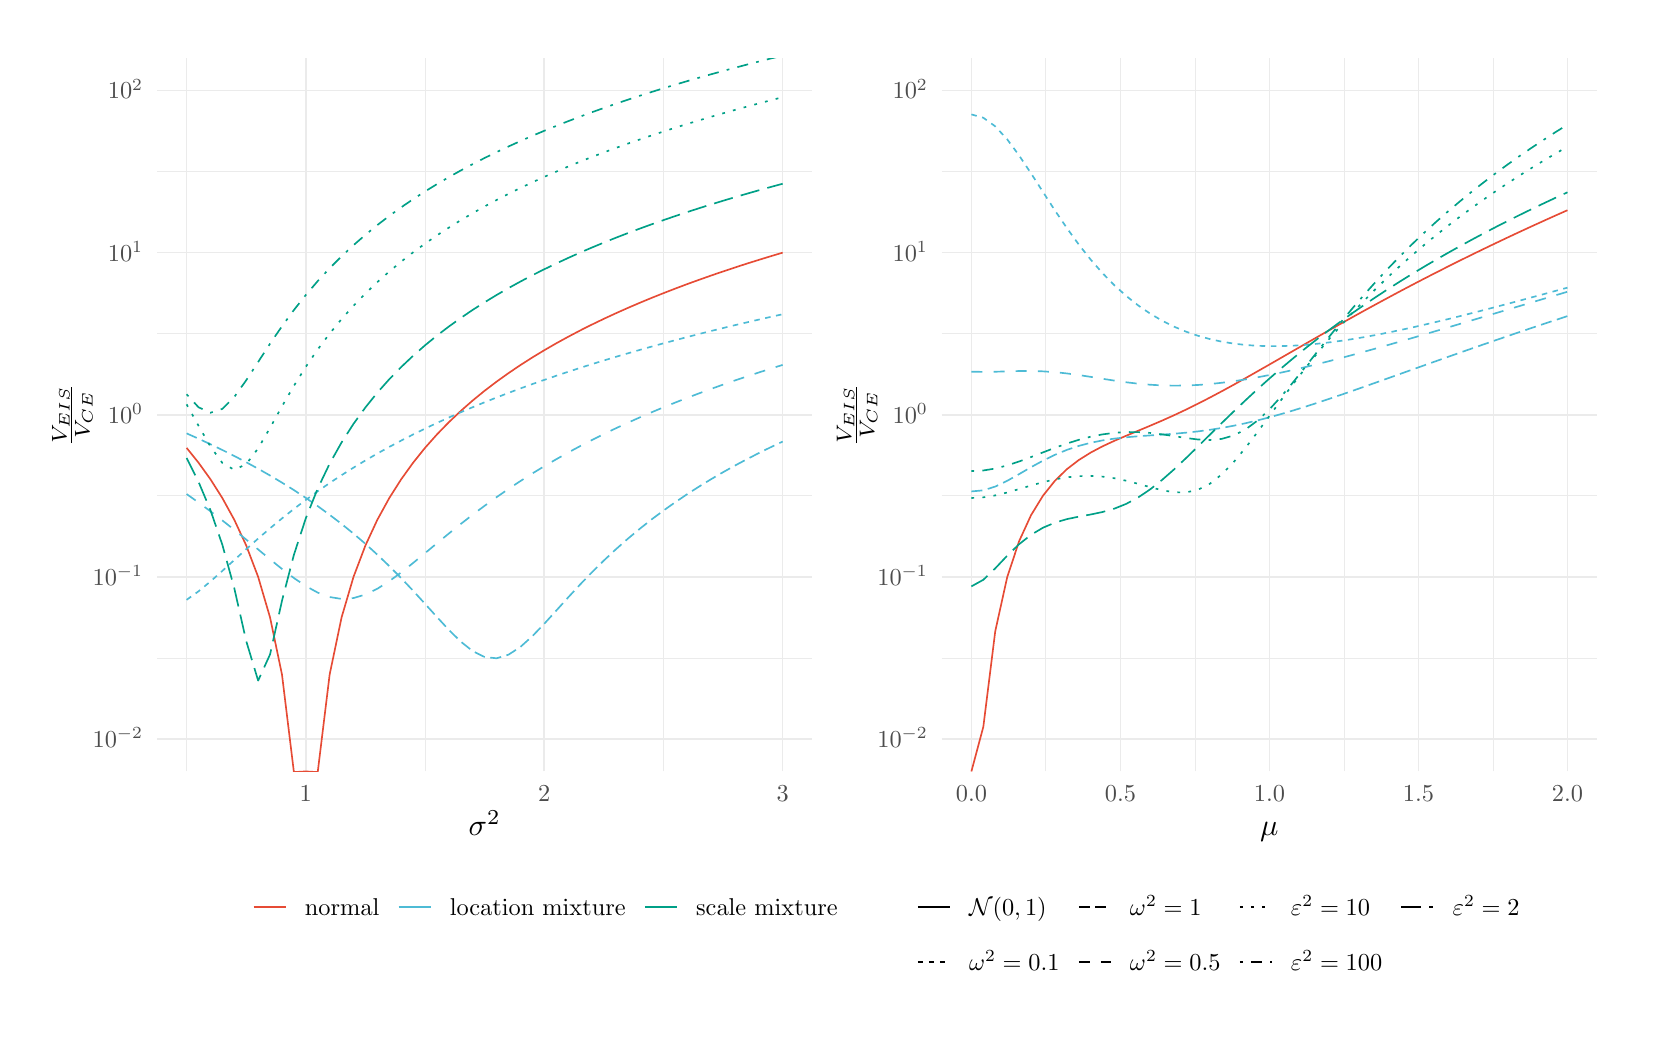
\begin{tikzpicture}[x=1pt,y=1pt]
\definecolor{fillColor}{RGB}{255,255,255}
\path[use as bounding box,fill=fillColor,fill opacity=0.00] (0,0) rectangle (578.16,361.35);
\begin{scope}
\path[clip] ( 46.66, 92.59) rectangle (283.58,350.35);
\definecolor{drawColor}{gray}{0.92}

\path[draw=drawColor,line width= 0.3pt,line join=round] ( 46.66,133.60) --
	(283.58,133.60);

\path[draw=drawColor,line width= 0.3pt,line join=round] ( 46.66,192.18) --
	(283.58,192.18);

\path[draw=drawColor,line width= 0.3pt,line join=round] ( 46.66,250.76) --
	(283.58,250.76);

\path[draw=drawColor,line width= 0.3pt,line join=round] ( 46.66,309.34) --
	(283.58,309.34);

\path[draw=drawColor,line width= 0.3pt,line join=round] ( 57.43, 92.59) --
	( 57.43,350.35);

\path[draw=drawColor,line width= 0.3pt,line join=round] (143.58, 92.59) --
	(143.58,350.35);

\path[draw=drawColor,line width= 0.3pt,line join=round] (229.74, 92.59) --
	(229.74,350.35);

\path[draw=drawColor,line width= 0.6pt,line join=round] ( 46.66,104.31) --
	(283.58,104.31);

\path[draw=drawColor,line width= 0.6pt,line join=round] ( 46.66,162.89) --
	(283.58,162.89);

\path[draw=drawColor,line width= 0.6pt,line join=round] ( 46.66,221.47) --
	(283.58,221.47);

\path[draw=drawColor,line width= 0.6pt,line join=round] ( 46.66,280.05) --
	(283.58,280.05);

\path[draw=drawColor,line width= 0.6pt,line join=round] ( 46.66,338.63) --
	(283.58,338.63);

\path[draw=drawColor,line width= 0.6pt,line join=round] (100.51, 92.59) --
	(100.51,350.35);

\path[draw=drawColor,line width= 0.6pt,line join=round] (186.66, 92.59) --
	(186.66,350.35);

\path[draw=drawColor,line width= 0.6pt,line join=round] (272.81, 92.59) --
	(272.81,350.35);
\definecolor{drawColor}{RGB}{230,75,53}

\path[draw=drawColor,line width= 0.6pt,line join=round] ( 57.43,209.51) --
	( 61.74,204.15) --
	( 66.05,198.16) --
	( 70.35,191.37) --
	( 74.66,183.52) --
	( 78.97,174.25) --
	( 83.28,162.89) --
	( 87.58,148.25) --
	( 91.89,127.62) --
	( 96.20, 92.35) --
	(100.51, 92.59) --
	(104.81, 92.35) --
	(109.12,127.62) --
	(113.43,148.25) --
	(117.74,162.89) --
	(122.05,174.25) --
	(126.35,183.52) --
	(130.66,191.37) --
	(134.97,198.16) --
	(139.28,204.15) --
	(143.58,209.51) --
	(147.89,214.36) --
	(152.20,218.79) --
	(156.51,222.86) --
	(160.81,226.63) --
	(165.12,230.15) --
	(169.43,233.43) --
	(173.74,236.51) --
	(178.04,239.42) --
	(182.35,242.17) --
	(186.66,244.78) --
	(190.97,247.27) --
	(195.27,249.63) --
	(199.58,251.90) --
	(203.89,254.06) --
	(208.20,256.14) --
	(212.50,258.13) --
	(216.81,260.05) --
	(221.12,261.90) --
	(225.43,263.69) --
	(229.74,265.41) --
	(234.04,267.08) --
	(238.35,268.70) --
	(242.66,270.26) --
	(246.97,271.78) --
	(251.27,273.26) --
	(255.58,274.69) --
	(259.89,276.09) --
	(264.20,277.44) --
	(268.50,278.76) --
	(272.81,280.05);
\definecolor{drawColor}{RGB}{77,187,213}

\path[draw=drawColor,line width= 0.6pt,dash pattern=on 2pt off 2pt ,line join=round] ( 57.43,154.60) --
	( 61.74,157.67) --
	( 66.05,161.24) --
	( 70.35,165.06) --
	( 74.66,168.99) --
	( 78.97,172.90) --
	( 83.28,176.74) --
	( 87.58,180.45) --
	( 91.89,184.02) --
	( 96.20,187.44) --
	(100.51,190.71) --
	(104.81,193.83) --
	(109.12,196.81) --
	(113.43,199.65) --
	(117.74,202.37) --
	(122.05,204.97) --
	(126.35,207.46) --
	(130.66,209.85) --
	(134.97,212.14) --
	(139.28,214.35) --
	(143.58,216.47) --
	(147.89,218.51) --
	(152.20,220.48) --
	(156.51,222.38) --
	(160.81,224.21) --
	(165.12,225.99) --
	(169.43,227.70) --
	(173.74,229.37) --
	(178.04,230.98) --
	(182.35,232.55) --
	(186.66,234.07) --
	(190.97,235.55) --
	(195.27,236.99) --
	(199.58,238.40) --
	(203.89,239.76) --
	(208.20,241.09) --
	(212.50,242.39) --
	(216.81,243.65) --
	(221.12,244.89) --
	(225.43,246.10) --
	(229.74,247.28) --
	(234.04,248.43) --
	(238.35,249.56) --
	(242.66,250.67) --
	(246.97,251.75) --
	(251.27,252.81) --
	(255.58,253.85) --
	(259.89,254.86) --
	(264.20,255.86) --
	(268.50,256.84) --
	(272.81,257.80);

\path[draw=drawColor,line width= 0.6pt,dash pattern=on 4pt off 2pt ,line join=round] ( 57.43,214.75) --
	( 61.74,212.82) --
	( 66.05,210.82) --
	( 70.35,208.74) --
	( 74.66,206.58) --
	( 78.97,204.32) --
	( 83.28,201.97) --
	( 87.58,199.52) --
	( 91.89,196.95) --
	( 96.20,194.26) --
	(100.51,191.43) --
	(104.81,188.46) --
	(109.12,185.32) --
	(113.43,182.02) --
	(117.74,178.52) --
	(122.05,174.83) --
	(126.35,170.92) --
	(130.66,166.79) --
	(134.97,162.44) --
	(139.28,157.88) --
	(143.58,153.16) --
	(147.89,148.39) --
	(152.20,143.73) --
	(156.51,139.49) --
	(160.81,136.06) --
	(165.12,133.94) --
	(169.43,133.47) --
	(173.74,134.77) --
	(178.04,137.57) --
	(182.35,141.45) --
	(186.66,145.93) --
	(190.97,150.67) --
	(195.27,155.44) --
	(199.58,160.09) --
	(203.89,164.55) --
	(208.20,168.80) --
	(212.50,172.82) --
	(216.81,176.63) --
	(221.12,180.22) --
	(225.43,183.63) --
	(229.74,186.85) --
	(234.04,189.90) --
	(238.35,192.80) --
	(242.66,195.56) --
	(246.97,198.20) --
	(251.27,200.71) --
	(255.58,203.11) --
	(259.89,205.42) --
	(264.20,207.62) --
	(268.50,209.75) --
	(272.81,211.79);

\path[draw=drawColor,line width= 0.6pt,dash pattern=on 4pt off 4pt ,line join=round] ( 57.43,192.82) --
	( 61.74,189.77) --
	( 66.05,186.59) --
	( 70.35,183.29) --
	( 74.66,179.88) --
	( 78.97,176.37) --
	( 83.28,172.81) --
	( 87.58,169.24) --
	( 91.89,165.76) --
	( 96.20,162.48) --
	(100.51,159.56) --
	(104.81,157.21) --
	(109.12,155.61) --
	(113.43,154.92) --
	(117.74,155.24) --
	(122.05,156.51) --
	(126.35,158.60) --
	(130.66,161.33) --
	(134.97,164.50) --
	(139.28,167.92) --
	(143.58,171.47) --
	(147.89,175.04) --
	(152.20,178.57) --
	(156.51,182.02) --
	(160.81,185.37) --
	(165.12,188.59) --
	(169.43,191.69) --
	(173.74,194.66) --
	(178.04,197.51) --
	(182.35,200.25) --
	(186.66,202.87) --
	(190.97,205.38) --
	(195.27,207.80) --
	(199.58,210.12) --
	(203.89,212.35) --
	(208.20,214.50) --
	(212.50,216.57) --
	(216.81,218.56) --
	(221.12,220.49) --
	(225.43,222.36) --
	(229.74,224.16) --
	(234.04,225.90) --
	(238.35,227.59) --
	(242.66,229.23) --
	(246.97,230.82) --
	(251.27,232.37) --
	(255.58,233.87) --
	(259.89,235.33) --
	(264.20,236.75) --
	(268.50,238.14) --
	(272.81,239.49);
\definecolor{drawColor}{RGB}{0,160,135}

\path[draw=drawColor,line width= 0.6pt,dash pattern=on 1pt off 3pt ,line join=round] ( 57.43,225.24) --
	( 61.74,217.50) --
	( 66.05,210.00) --
	( 70.35,204.05) --
	( 74.66,201.56) --
	( 78.97,203.63) --
	( 83.28,209.33) --
	( 87.58,216.75) --
	( 91.89,224.51) --
	( 96.20,231.93) --
	(100.51,238.80) --
	(104.81,245.08) --
	(109.12,250.81) --
	(113.43,256.05) --
	(117.74,260.86) --
	(122.05,265.30) --
	(126.35,269.41) --
	(130.66,273.23) --
	(134.97,276.81) --
	(139.28,280.16) --
	(143.58,283.31) --
	(147.89,286.29) --
	(152.20,289.10) --
	(156.51,291.78) --
	(160.81,294.32) --
	(165.12,296.75) --
	(169.43,299.07) --
	(173.74,301.29) --
	(178.04,303.42) --
	(182.35,305.46) --
	(186.66,307.43) --
	(190.97,309.32) --
	(195.27,311.15) --
	(199.58,312.91) --
	(203.89,314.62) --
	(208.20,316.27) --
	(212.50,317.87) --
	(216.81,319.43) --
	(221.12,320.93) --
	(225.43,322.40) --
	(229.74,323.82) --
	(234.04,325.21) --
	(238.35,326.55) --
	(242.66,327.87) --
	(246.97,329.15) --
	(251.27,330.40) --
	(255.58,331.62) --
	(259.89,332.81) --
	(264.20,333.97) --
	(268.50,335.11) --
	(272.81,336.23);

\path[draw=drawColor,line width= 0.6pt,dash pattern=on 1pt off 3pt on 4pt off 3pt ,line join=round] ( 57.43,228.88) --
	( 61.74,224.18) --
	( 66.05,222.19) --
	( 70.35,223.60) --
	( 74.66,227.92) --
	( 78.97,233.93) --
	( 83.28,240.55) --
	( 87.58,247.16) --
	( 91.89,253.45) --
	( 96.20,259.32) --
	(100.51,264.75) --
	(104.81,269.78) --
	(109.12,274.43) --
	(113.43,278.74) --
	(117.74,282.75) --
	(122.05,286.50) --
	(126.35,290.02) --
	(130.66,293.32) --
	(134.97,296.43) --
	(139.28,299.37) --
	(143.58,302.16) --
	(147.89,304.81) --
	(152.20,307.34) --
	(156.51,309.75) --
	(160.81,312.05) --
	(165.12,314.26) --
	(169.43,316.38) --
	(173.74,318.41) --
	(178.04,320.37) --
	(182.35,322.26) --
	(186.66,324.08) --
	(190.97,325.84) --
	(195.27,327.54) --
	(199.58,329.19) --
	(203.89,330.79) --
	(208.20,332.33) --
	(212.50,333.84) --
	(216.81,335.30) --
	(221.12,336.72) --
	(225.43,338.10) --
	(229.74,339.45) --
	(234.04,340.76) --
	(238.35,342.04) --
	(242.66,343.29) --
	(246.97,344.51) --
	(251.27,345.70) --
	(255.58,346.86) --
	(259.89,348.00) --
	(264.20,349.11) --
	(268.50,350.20) --
	(272.81,351.26);

\path[draw=drawColor,line width= 0.6pt,dash pattern=on 7pt off 3pt ,line join=round] ( 57.43,205.84) --
	( 61.74,197.23) --
	( 66.05,186.99) --
	( 70.35,174.47) --
	( 74.66,158.79) --
	( 78.97,139.71) --
	( 83.28,125.40) --
	( 87.58,134.87) --
	( 91.89,154.24) --
	( 96.20,170.86) --
	(100.51,184.08) --
	(104.81,194.82) --
	(109.12,203.80) --
	(113.43,211.48) --
	(117.74,218.19) --
	(122.05,224.13) --
	(126.35,229.47) --
	(130.66,234.30) --
	(134.97,238.72) --
	(139.28,242.79) --
	(143.58,246.56) --
	(147.89,250.08) --
	(152.20,253.36) --
	(156.51,256.45) --
	(160.81,259.37) --
	(165.12,262.12) --
	(169.43,264.74) --
	(173.74,267.23) --
	(178.04,269.60) --
	(182.35,271.87) --
	(186.66,274.04) --
	(190.97,276.12) --
	(195.27,278.12) --
	(199.58,280.05) --
	(203.89,281.90) --
	(208.20,283.69) --
	(212.50,285.42) --
	(216.81,287.09) --
	(221.12,288.71) --
	(225.43,290.28) --
	(229.74,291.80) --
	(234.04,293.28) --
	(238.35,294.72) --
	(242.66,296.12) --
	(246.97,297.48) --
	(251.27,298.80) --
	(255.58,300.09) --
	(259.89,301.35) --
	(264.20,302.58) --
	(268.50,303.78) --
	(272.81,304.95);
\end{scope}
\begin{scope}
\path[clip] (  0.00,  0.00) rectangle (578.16,361.35);
\definecolor{drawColor}{gray}{0.30}

\node[text=drawColor,anchor=base east,inner sep=0pt, outer sep=0pt, scale=  0.88] at ( 41.71,101.28) {$10^{-2}$};

\node[text=drawColor,anchor=base east,inner sep=0pt, outer sep=0pt, scale=  0.88] at ( 41.71,159.86) {$10^{-1}$};

\node[text=drawColor,anchor=base east,inner sep=0pt, outer sep=0pt, scale=  0.88] at ( 41.71,218.44) {$10^{0}$};

\node[text=drawColor,anchor=base east,inner sep=0pt, outer sep=0pt, scale=  0.88] at ( 41.71,277.02) {$10^{1}$};

\node[text=drawColor,anchor=base east,inner sep=0pt, outer sep=0pt, scale=  0.88] at ( 41.71,335.60) {$10^{2}$};
\end{scope}
\begin{scope}
\path[clip] (  0.00,  0.00) rectangle (578.16,361.35);
\definecolor{drawColor}{gray}{0.30}

\node[text=drawColor,anchor=base,inner sep=0pt, outer sep=0pt, scale=  0.88] at (100.51, 81.58) {1};

\node[text=drawColor,anchor=base,inner sep=0pt, outer sep=0pt, scale=  0.88] at (186.66, 81.58) {2};

\node[text=drawColor,anchor=base,inner sep=0pt, outer sep=0pt, scale=  0.88] at (272.81, 81.58) {3};
\end{scope}
\begin{scope}
\path[clip] (  0.00,  0.00) rectangle (578.16,361.35);
\definecolor{drawColor}{RGB}{0,0,0}

\node[text=drawColor,anchor=base,inner sep=0pt, outer sep=0pt, scale=  1.10] at (165.12, 69.55) {$\sigma^2$};
\end{scope}
\begin{scope}
\path[clip] (  0.00,  0.00) rectangle (578.16,361.35);
\definecolor{drawColor}{RGB}{0,0,0}

\node[text=drawColor,rotate= 90.00,anchor=base,inner sep=0pt, outer sep=0pt, scale=  1.10] at ( 18.58,221.47) {$\frac{V_{EIS}}{V_{CE}}$};
\end{scope}
\begin{scope}
\path[clip] (330.24, 92.59) rectangle (567.16,350.35);
\definecolor{drawColor}{gray}{0.92}

\path[draw=drawColor,line width= 0.3pt,line join=round] (330.24,133.60) --
	(567.16,133.60);

\path[draw=drawColor,line width= 0.3pt,line join=round] (330.24,192.18) --
	(567.16,192.18);

\path[draw=drawColor,line width= 0.3pt,line join=round] (330.24,250.76) --
	(567.16,250.76);

\path[draw=drawColor,line width= 0.3pt,line join=round] (330.24,309.34) --
	(567.16,309.34);

\path[draw=drawColor,line width= 0.3pt,line join=round] (367.93, 92.59) --
	(367.93,350.35);

\path[draw=drawColor,line width= 0.3pt,line join=round] (421.78, 92.59) --
	(421.78,350.35);

\path[draw=drawColor,line width= 0.3pt,line join=round] (475.62, 92.59) --
	(475.62,350.35);

\path[draw=drawColor,line width= 0.3pt,line join=round] (529.47, 92.59) --
	(529.47,350.35);

\path[draw=drawColor,line width= 0.6pt,line join=round] (330.24,104.31) --
	(567.16,104.31);

\path[draw=drawColor,line width= 0.6pt,line join=round] (330.24,162.89) --
	(567.16,162.89);

\path[draw=drawColor,line width= 0.6pt,line join=round] (330.24,221.47) --
	(567.16,221.47);

\path[draw=drawColor,line width= 0.6pt,line join=round] (330.24,280.05) --
	(567.16,280.05);

\path[draw=drawColor,line width= 0.6pt,line join=round] (330.24,338.63) --
	(567.16,338.63);

\path[draw=drawColor,line width= 0.6pt,line join=round] (341.01, 92.59) --
	(341.01,350.35);

\path[draw=drawColor,line width= 0.6pt,line join=round] (394.86, 92.59) --
	(394.86,350.35);

\path[draw=drawColor,line width= 0.6pt,line join=round] (448.70, 92.59) --
	(448.70,350.35);

\path[draw=drawColor,line width= 0.6pt,line join=round] (502.55, 92.59) --
	(502.55,350.35);

\path[draw=drawColor,line width= 0.6pt,line join=round] (556.39, 92.59) --
	(556.39,350.35);
\definecolor{drawColor}{RGB}{230,75,53}

\path[draw=drawColor,line width= 0.6pt,line join=round] (341.01, 92.59) --
	(345.32,108.70) --
	(349.63,143.25) --
	(353.93,162.71) --
	(358.24,175.76) --
	(362.55,185.16) --
	(366.86,192.20) --
	(371.16,197.58) --
	(375.47,201.77) --
	(379.78,205.09) --
	(384.09,207.79) --
	(388.39,210.07) --
	(392.70,212.07) --
	(397.01,213.92) --
	(401.32,215.72) --
	(405.63,217.52) --
	(409.93,219.37) --
	(414.24,221.30) --
	(418.55,223.33) --
	(422.86,225.46) --
	(427.16,227.67) --
	(431.47,229.96) --
	(435.78,232.31) --
	(440.09,234.72) --
	(444.39,237.16) --
	(448.70,239.62) --
	(453.01,242.10) --
	(457.32,244.58) --
	(461.62,247.06) --
	(465.93,249.53) --
	(470.24,251.98) --
	(474.55,254.41) --
	(478.85,256.81) --
	(483.16,259.20) --
	(487.47,261.55) --
	(491.78,263.88) --
	(496.08,266.18) --
	(500.39,268.45) --
	(504.70,270.69) --
	(509.01,272.90) --
	(513.32,275.08) --
	(517.62,277.23) --
	(521.93,279.36) --
	(526.24,281.45) --
	(530.55,283.52) --
	(534.85,285.56) --
	(539.16,287.58) --
	(543.47,289.57) --
	(547.78,291.53) --
	(552.08,293.47) --
	(556.39,295.38);
\definecolor{drawColor}{RGB}{77,187,213}

\path[draw=drawColor,line width= 0.6pt,dash pattern=on 2pt off 2pt ,line join=round] (341.01,330.00) --
	(345.32,328.79) --
	(349.63,325.69) --
	(353.93,321.01) --
	(358.24,315.20) --
	(362.55,308.73) --
	(366.86,302.01) --
	(371.16,295.35) --
	(375.47,288.98) --
	(379.78,283.03) --
	(384.09,277.57) --
	(388.39,272.65) --
	(392.70,268.24) --
	(397.01,264.36) --
	(401.32,260.95) --
	(405.63,258.00) --
	(409.93,255.47) --
	(414.24,253.31) --
	(418.55,251.51) --
	(422.86,250.03) --
	(427.16,248.83) --
	(431.47,247.89) --
	(435.78,247.19) --
	(440.09,246.69) --
	(444.39,246.39) --
	(448.70,246.26) --
	(453.01,246.28) --
	(457.32,246.44) --
	(461.62,246.72) --
	(465.93,247.12) --
	(470.24,247.61) --
	(474.55,248.19) --
	(478.85,248.84) --
	(483.16,249.57) --
	(487.47,250.36) --
	(491.78,251.21) --
	(496.08,252.10) --
	(500.39,253.04) --
	(504.70,254.02) --
	(509.01,255.03) --
	(513.32,256.06) --
	(517.62,257.13) --
	(521.93,258.22) --
	(526.24,259.32) --
	(530.55,260.45) --
	(534.85,261.58) --
	(539.16,262.73) --
	(543.47,263.89) --
	(547.78,265.05) --
	(552.08,266.23) --
	(556.39,267.40);

\path[draw=drawColor,line width= 0.6pt,dash pattern=on 4pt off 2pt ,line join=round] (341.01,193.77) --
	(345.32,194.16) --
	(349.63,195.53) --
	(353.93,197.59) --
	(358.24,200.02) --
	(362.55,202.52) --
	(366.86,204.88) --
	(371.16,206.98) --
	(375.47,208.76) --
	(379.78,210.21) --
	(384.09,211.34) --
	(388.39,212.21) --
	(392.70,212.86) --
	(397.01,213.34) --
	(401.32,213.71) --
	(405.63,214.01) --
	(409.93,214.30) --
	(414.24,214.62) --
	(418.55,215.00) --
	(422.86,215.46) --
	(427.16,216.03) --
	(431.47,216.71) --
	(435.78,217.51) --
	(440.09,218.42) --
	(444.39,219.43) --
	(448.70,220.55) --
	(453.01,221.75) --
	(457.32,223.03) --
	(461.62,224.37) --
	(465.93,225.76) --
	(470.24,227.20) --
	(474.55,228.67) --
	(478.85,230.16) --
	(483.16,231.68) --
	(487.47,233.21) --
	(491.78,234.74) --
	(496.08,236.28) --
	(500.39,237.82) --
	(504.70,239.36) --
	(509.01,240.89) --
	(513.32,242.42) --
	(517.62,243.94) --
	(521.93,245.45) --
	(526.24,246.95) --
	(530.55,248.44) --
	(534.85,249.92) --
	(539.16,251.38) --
	(543.47,252.84) --
	(547.78,254.28) --
	(552.08,255.70) --
	(556.39,257.12);

\path[draw=drawColor,line width= 0.6pt,dash pattern=on 4pt off 4pt ,line join=round] (341.01,237.04) --
	(345.32,236.96) --
	(349.63,237.02) --
	(353.93,237.15) --
	(358.24,237.27) --
	(362.55,237.29) --
	(366.86,237.16) --
	(371.16,236.87) --
	(375.47,236.41) --
	(379.78,235.83) --
	(384.09,235.17) --
	(388.39,234.48) --
	(392.70,233.81) --
	(397.01,233.20) --
	(401.32,232.70) --
	(405.63,232.32) --
	(409.93,232.08) --
	(414.24,231.99) --
	(418.55,232.05) --
	(422.86,232.24) --
	(427.16,232.57) --
	(431.47,233.03) --
	(435.78,233.59) --
	(440.09,234.25) --
	(444.39,235.00) --
	(448.70,235.83) --
	(453.01,236.72) --
	(457.32,237.68) --
	(461.62,238.69) --
	(465.93,239.74) --
	(470.24,240.84) --
	(474.55,241.97) --
	(478.85,243.12) --
	(483.16,244.31) --
	(487.47,245.51) --
	(491.78,246.74) --
	(496.08,247.98) --
	(500.39,249.23) --
	(504.70,250.50) --
	(509.01,251.77) --
	(513.32,253.05) --
	(517.62,254.33) --
	(521.93,255.62) --
	(526.24,256.91) --
	(530.55,258.20) --
	(534.85,259.49) --
	(539.16,260.78) --
	(543.47,262.07) --
	(547.78,263.36) --
	(552.08,264.64) --
	(556.39,265.92);
\definecolor{drawColor}{RGB}{0,160,135}

\path[draw=drawColor,line width= 0.6pt,dash pattern=on 1pt off 3pt ,line join=round] (341.01,191.40) --
	(345.32,191.63) --
	(349.63,192.33) --
	(353.93,193.38) --
	(358.24,194.62) --
	(362.55,195.91) --
	(366.86,197.11) --
	(371.16,198.12) --
	(375.47,198.86) --
	(379.78,199.29) --
	(384.09,199.38) --
	(388.39,199.12) --
	(392.70,198.52) --
	(397.01,197.62) --
	(401.32,196.51) --
	(405.63,195.30) --
	(409.93,194.20) --
	(414.24,193.46) --
	(418.55,193.41) --
	(422.86,194.37) --
	(427.16,196.53) --
	(431.47,199.92) --
	(435.78,204.36) --
	(440.09,209.55) --
	(444.39,215.20) --
	(448.70,221.04) --
	(453.01,226.90) --
	(457.32,232.66) --
	(461.62,238.24) --
	(465.93,243.62) --
	(470.24,248.79) --
	(474.55,253.73) --
	(478.85,258.45) --
	(483.16,262.97) --
	(487.47,267.30) --
	(491.78,271.45) --
	(496.08,275.42) --
	(500.39,279.23) --
	(504.70,282.90) --
	(509.01,286.43) --
	(513.32,289.83) --
	(517.62,293.11) --
	(521.93,296.28) --
	(526.24,299.34) --
	(530.55,302.31) --
	(534.85,305.18) --
	(539.16,307.96) --
	(543.47,310.67) --
	(547.78,313.30) --
	(552.08,315.85) --
	(556.39,318.34);

\path[draw=drawColor,line width= 0.6pt,dash pattern=on 1pt off 3pt on 4pt off 3pt ,line join=round] (341.01,201.14) --
	(345.32,201.34) --
	(349.63,202.04) --
	(353.93,203.16) --
	(358.24,204.58) --
	(362.55,206.19) --
	(366.86,207.87) --
	(371.16,209.52) --
	(375.47,211.05) --
	(379.78,212.41) --
	(384.09,213.53) --
	(388.39,214.38) --
	(392.70,214.95) --
	(397.01,215.22) --
	(401.32,215.20) --
	(405.63,214.91) --
	(409.93,214.40) --
	(414.24,213.75) --
	(418.55,213.07) --
	(422.86,212.54) --
	(427.16,212.35) --
	(431.47,212.76) --
	(435.78,213.99) --
	(440.09,216.18) --
	(444.39,219.36) --
	(448.70,223.41) --
	(453.01,228.13) --
	(457.32,233.29) --
	(461.62,238.69) --
	(465.93,244.16) --
	(470.24,249.60) --
	(474.55,254.93) --
	(478.85,260.10) --
	(483.16,265.10) --
	(487.47,269.91) --
	(491.78,274.53) --
	(496.08,278.97) --
	(500.39,283.23) --
	(504.70,287.32) --
	(509.01,291.25) --
	(513.32,295.02) --
	(517.62,298.66) --
	(521.93,302.17) --
	(526.24,305.54) --
	(530.55,308.81) --
	(534.85,311.96) --
	(539.16,315.01) --
	(543.47,317.96) --
	(547.78,320.82) --
	(552.08,323.60) --
	(556.39,326.29);

\path[draw=drawColor,line width= 0.6pt,dash pattern=on 7pt off 3pt ,line join=round] (341.01,159.46) --
	(345.32,161.84) --
	(349.63,165.97) --
	(353.93,170.53) --
	(358.24,174.69) --
	(362.55,178.08) --
	(366.86,180.65) --
	(371.16,182.48) --
	(375.47,183.75) --
	(379.78,184.65) --
	(384.09,185.43) --
	(388.39,186.33) --
	(392.70,187.56) --
	(397.01,189.30) --
	(401.32,191.62) --
	(405.63,194.53) --
	(409.93,197.94) --
	(414.24,201.73) --
	(418.55,205.79) --
	(422.86,209.99) --
	(427.16,214.24) --
	(431.47,218.48) --
	(435.78,222.65) --
	(440.09,226.73) --
	(444.39,230.71) --
	(448.70,234.56) --
	(453.01,238.30) --
	(457.32,241.91) --
	(461.62,245.41) --
	(465.93,248.80) --
	(470.24,252.07) --
	(474.55,255.25) --
	(478.85,258.33) --
	(483.16,261.31) --
	(487.47,264.21) --
	(491.78,267.03) --
	(496.08,269.76) --
	(500.39,272.43) --
	(504.70,275.03) --
	(509.01,277.56) --
	(513.32,280.02) --
	(517.62,282.43) --
	(521.93,284.78) --
	(526.24,287.08) --
	(530.55,289.33) --
	(534.85,291.53) --
	(539.16,293.68) --
	(543.47,295.78) --
	(547.78,297.85) --
	(552.08,299.87) --
	(556.39,301.85);
\end{scope}
\begin{scope}
\path[clip] (  0.00,  0.00) rectangle (578.16,361.35);
\definecolor{drawColor}{gray}{0.30}

\node[text=drawColor,anchor=base east,inner sep=0pt, outer sep=0pt, scale=  0.88] at (325.29,101.28) {$10^{-2}$};

\node[text=drawColor,anchor=base east,inner sep=0pt, outer sep=0pt, scale=  0.88] at (325.29,159.86) {$10^{-1}$};

\node[text=drawColor,anchor=base east,inner sep=0pt, outer sep=0pt, scale=  0.88] at (325.29,218.44) {$10^{0}$};

\node[text=drawColor,anchor=base east,inner sep=0pt, outer sep=0pt, scale=  0.88] at (325.29,277.02) {$10^{1}$};

\node[text=drawColor,anchor=base east,inner sep=0pt, outer sep=0pt, scale=  0.88] at (325.29,335.60) {$10^{2}$};
\end{scope}
\begin{scope}
\path[clip] (  0.00,  0.00) rectangle (578.16,361.35);
\definecolor{drawColor}{gray}{0.30}

\node[text=drawColor,anchor=base,inner sep=0pt, outer sep=0pt, scale=  0.88] at (341.01, 81.58) {0.0};

\node[text=drawColor,anchor=base,inner sep=0pt, outer sep=0pt, scale=  0.88] at (394.86, 81.58) {0.5};

\node[text=drawColor,anchor=base,inner sep=0pt, outer sep=0pt, scale=  0.88] at (448.70, 81.58) {1.0};

\node[text=drawColor,anchor=base,inner sep=0pt, outer sep=0pt, scale=  0.88] at (502.55, 81.58) {1.5};

\node[text=drawColor,anchor=base,inner sep=0pt, outer sep=0pt, scale=  0.88] at (556.39, 81.58) {2.0};
\end{scope}
\begin{scope}
\path[clip] (  0.00,  0.00) rectangle (578.16,361.35);
\definecolor{drawColor}{RGB}{0,0,0}

\node[text=drawColor,anchor=base,inner sep=0pt, outer sep=0pt, scale=  1.10] at (448.70, 69.55) {$\mu$};
\end{scope}
\begin{scope}
\path[clip] (  0.00,  0.00) rectangle (578.16,361.35);
\definecolor{drawColor}{RGB}{0,0,0}

\node[text=drawColor,rotate= 90.00,anchor=base,inner sep=0pt, outer sep=0pt, scale=  1.10] at (302.16,221.47) {$\frac{V_{EIS}}{V_{CE}}$};
\end{scope}
\begin{scope}
\path[clip] (  0.00,  0.00) rectangle (578.16,361.35);
\definecolor{drawColor}{RGB}{230,75,53}

\path[draw=drawColor,line width= 0.6pt,line join=round] ( 81.65, 43.68) -- ( 93.22, 43.68);
\end{scope}
\begin{scope}
\path[clip] (  0.00,  0.00) rectangle (578.16,361.35);
\definecolor{drawColor}{RGB}{77,187,213}

\path[draw=drawColor,line width= 0.6pt,line join=round] (134.01, 43.68) -- (145.58, 43.68);
\end{scope}
\begin{scope}
\path[clip] (  0.00,  0.00) rectangle (578.16,361.35);
\definecolor{drawColor}{RGB}{0,160,135}

\path[draw=drawColor,line width= 0.6pt,line join=round] (223.03, 43.68) -- (234.60, 43.68);
\end{scope}
\begin{scope}
\path[clip] (  0.00,  0.00) rectangle (578.16,361.35);
\definecolor{drawColor}{RGB}{0,0,0}

\node[text=drawColor,anchor=base west,inner sep=0pt, outer sep=0pt, scale=  0.88] at (100.16, 40.65) {normal};
\end{scope}
\begin{scope}
\path[clip] (  0.00,  0.00) rectangle (578.16,361.35);
\definecolor{drawColor}{RGB}{0,0,0}

\node[text=drawColor,anchor=base west,inner sep=0pt, outer sep=0pt, scale=  0.88] at (152.52, 40.65) {location mixture};
\end{scope}
\begin{scope}
\path[clip] (  0.00,  0.00) rectangle (578.16,361.35);
\definecolor{drawColor}{RGB}{0,0,0}

\node[text=drawColor,anchor=base west,inner sep=0pt, outer sep=0pt, scale=  0.88] at (241.54, 40.65) {scale mixture};
\end{scope}
\begin{scope}
\path[clip] (  0.00,  0.00) rectangle (578.16,361.35);
\definecolor{drawColor}{RGB}{0,0,0}

\path[draw=drawColor,line width= 0.6pt,line join=round] (321.64, 43.68) -- (333.20, 43.68);
\end{scope}
\begin{scope}
\path[clip] (  0.00,  0.00) rectangle (578.16,361.35);
\definecolor{drawColor}{RGB}{0,0,0}

\path[draw=drawColor,line width= 0.6pt,dash pattern=on 2pt off 2pt ,line join=round] (321.64, 23.73) -- (333.20, 23.73);
\end{scope}
\begin{scope}
\path[clip] (  0.00,  0.00) rectangle (578.16,361.35);
\definecolor{drawColor}{RGB}{0,0,0}

\path[draw=drawColor,line width= 0.6pt,dash pattern=on 4pt off 2pt ,line join=round] (379.81, 43.68) -- (391.37, 43.68);
\end{scope}
\begin{scope}
\path[clip] (  0.00,  0.00) rectangle (578.16,361.35);
\definecolor{drawColor}{RGB}{0,0,0}

\path[draw=drawColor,line width= 0.6pt,dash pattern=on 4pt off 4pt ,line join=round] (379.81, 23.73) -- (391.37, 23.73);
\end{scope}
\begin{scope}
\path[clip] (  0.00,  0.00) rectangle (578.16,361.35);
\definecolor{drawColor}{RGB}{0,0,0}

\path[draw=drawColor,line width= 0.6pt,dash pattern=on 1pt off 3pt ,line join=round] (437.98, 43.68) -- (449.55, 43.68);
\end{scope}
\begin{scope}
\path[clip] (  0.00,  0.00) rectangle (578.16,361.35);
\definecolor{drawColor}{RGB}{0,0,0}

\path[draw=drawColor,line width= 0.6pt,dash pattern=on 1pt off 3pt on 4pt off 3pt ,line join=round] (437.98, 23.73) -- (449.55, 23.73);
\end{scope}
\begin{scope}
\path[clip] (  0.00,  0.00) rectangle (578.16,361.35);
\definecolor{drawColor}{RGB}{0,0,0}

\path[draw=drawColor,line width= 0.6pt,dash pattern=on 7pt off 3pt ,line join=round] (496.42, 43.68) -- (507.98, 43.68);
\end{scope}
\begin{scope}
\path[clip] (  0.00,  0.00) rectangle (578.16,361.35);
\definecolor{drawColor}{RGB}{0,0,0}

\node[text=drawColor,anchor=base west,inner sep=0pt, outer sep=0pt, scale=  0.88] at (340.15, 40.65) {$\mathcal N (0, 1)$};
\end{scope}
\begin{scope}
\path[clip] (  0.00,  0.00) rectangle (578.16,361.35);
\definecolor{drawColor}{RGB}{0,0,0}

\node[text=drawColor,anchor=base west,inner sep=0pt, outer sep=0pt, scale=  0.88] at (340.15, 20.70) {$\omega^2 = 0.1$};
\end{scope}
\begin{scope}
\path[clip] (  0.00,  0.00) rectangle (578.16,361.35);
\definecolor{drawColor}{RGB}{0,0,0}

\node[text=drawColor,anchor=base west,inner sep=0pt, outer sep=0pt, scale=  0.88] at (398.32, 40.65) {$\omega^2 = 1$};
\end{scope}
\begin{scope}
\path[clip] (  0.00,  0.00) rectangle (578.16,361.35);
\definecolor{drawColor}{RGB}{0,0,0}

\node[text=drawColor,anchor=base west,inner sep=0pt, outer sep=0pt, scale=  0.88] at (398.32, 20.70) {$\omega^2= 0.5$};
\end{scope}
\begin{scope}
\path[clip] (  0.00,  0.00) rectangle (578.16,361.35);
\definecolor{drawColor}{RGB}{0,0,0}

\node[text=drawColor,anchor=base west,inner sep=0pt, outer sep=0pt, scale=  0.88] at (456.49, 40.65) {$\varepsilon^2 = 10$};
\end{scope}
\begin{scope}
\path[clip] (  0.00,  0.00) rectangle (578.16,361.35);
\definecolor{drawColor}{RGB}{0,0,0}

\node[text=drawColor,anchor=base west,inner sep=0pt, outer sep=0pt, scale=  0.88] at (456.49, 20.70) {$\varepsilon^2 = 100$};
\end{scope}
\begin{scope}
\path[clip] (  0.00,  0.00) rectangle (578.16,361.35);
\definecolor{drawColor}{RGB}{0,0,0}

\node[text=drawColor,anchor=base west,inner sep=0pt, outer sep=0pt, scale=  0.88] at (514.93, 40.65) {$\varepsilon^2 = 2$};
\end{scope}
\end{tikzpicture}
%
        }
        \caption{Asymptotic relative efficiency $\frac{V_{\eis}}{V_{\ce}}$ for the normal distribution from \Cref{ex:univ-gaussian-s2-fixed} (left hand side) and \Cref{ex:univ-gaussian-mu-fixed} (right hand side). Here $\P$ is either the standard normal distribution, a Gaussian location mixture, or a Gaussian scale mixture. $\G_{\psi}$ is the normal distribution $\mathcal N(\mu, \sigma^{2})$, where either $\sigma^{2}$ is fixed (left) and $\mu$ determined by the \gls{cem} / \gls{eis}, or the other way around (right). Notice the log scale of the $y$-axis. As $\mu$ or $\sigma^{2}$ get close to their true values, \gls{eis} outperforms the \gls{cem} in terms of asymptotic variance, see \Cref{prop:eis-finite-sample}. {\color{red} todo: clean up figure legend / linetype, order eps and omega, add global $\sigma^{2}$ choosen by estimating both parameters at the same time?}}
        \label{fig:are}
    \end{figure}

    
    \paragraph{Normal distribution}
    If $\P = \mathcal N(0, \tau^{2})$ is a normal distribution, this reduces to
    \begin{align*}
        V_{\eis} &= \frac{5}{2} \left( \frac{\tau^{2}}{\sigma^{2}} - 1 \right)^{2} \frac{\sigma^{2}}{\tau^{2}} = \frac{5}{2} \frac{\left( V_{\ce} - 1\right)^{2}}{V_{\ce}}
    \end{align*}
    and so for $\tau^{2} = \sigma^{2}$ $\hpeis$ converges faster than the standard $\mathcal O( N^{-\frac{1}{2}})$ rate. Indeed in this case $\hpeis = \peis$ a.s. for $N > 1$, see \Cref{prop:eis-finite-sample}.

    %For importance sampling to be consistent, it is necessary that $\sigma^{2} > \frac{\tau^{2}}{2}$. The left-hand side of \Cref{fig:are} displays the behavior of the relative efficiency
    %$$
    %\frac{V_{\eis}}{V_{\ce}} = \frac{5}{2} \frac{(V_{\ce} - 1)^{2}}{V_{\ce}^{2}} = \frac{5}{2} \left( 1 - \frac{2}{V_{\ce}} + \frac{1}{V_{\ce}^2} \right).
    %$$
    
    \paragraph{Gaussian location mixture}
    Consider now the case where $\P = \frac{1}{2} \mathcal N(-1, \omega^{2}) + \frac{1}{2}\mathcal N(1, \omega^{2})$ is a Gaussian location mixture. The second moment is $\tau^{2} = 1 + \omega^{2} = -\frac{1}{2\pce}$. Unfortunately, there is no closed-form expression for many of the terms required for the analysis \gls{eis}. Instead, we resort to a simulation study to determine the asymptotic variances and relative efficiencies for three different values of $\omega^{2} \in \{0.1, 0.5, 1.0\}$. 
    
    To this end we draw $M = 100$ times from the distribution of $\hpce$ and $\hpeis$, where we use $N=1000$ samples from the tractable $\P$ as importance samples. We only iterate a single time for both procedures. From individual estimates, we estimate the asymptotic variances $V_{\ce}$ and $V_{\eis}$ by the respective empirical variances, and determine the relative efficiency of \gls{eis} over the \gls{cem} as $ \frac{V_{\eis}}{V_{\ce}}$. Again, we vary the fixed variance of the proposals, $\sigma^{2}$, from $\frac{1}{2}$ to $3$. 
    \todo{discuss MC error of this estimate, small enough to ignore?}
    
    \paragraph{Gaussian scale mixture}
    Finally we consider $\P = \frac{1}{2} \left(\mathcal N \left( 0, 1 \right) + \mathcal N (0, \varepsilon^{-2}) \right)$ for $\varepsilon^{2} \in \{2, 10, 100\}$, a scale mixture similar to the one seen in \Cref{ex:la_failure}. Contrary to that example, we choose $\varepsilon$ big, making the $\mathcal N(0,1)$ component the one with large variance, to make importance sampling with $\sigma^{2}$ in the range considered consistent. 
    Here $\tau^{2} = \frac{1}{2} + \frac{1}{2\varepsilon^{2}}$. 
    Again, we estimate the asymptotic $V_{\eis}$ in the same way as for the Gaussian location mixture, with $M=100$ estimates using $N=1000$ samples each. 
\end{example}

Note that for fixed $\sigma^{2}$ the asymptotic variance of the \acrshort{cem} $V_{\ce}$ is the same in all of the examples considered, as we sample directly from the tractable $\P$, so $V_{\ce}$ only depends on $\P$ through its second moment $\tau^{2}$. 
The asymptotic variance of \acrshort{eis} however depends on both $\tau^{2}$, as well as $\gamma$, which depends on global properties of $\P$. 

From the left-hand side of \Cref{fig:are} we can observe that in the case of $\P = \mathcal N(0,1)$ \acrshort{eis} has smaller asymptotic variance compared to the \acrshort{cem}, as long as $\sigma^{2}$ is not heavily misspecified. Indeed, if $\sigma^{2} = 1$ is correctly specified, by \Cref{prop:eis-finite-sample}, \acrshort{eis} has asymptotic variance $0$ and converges already for a single sample. 

Consider now the case where $\P$ is a Gaussian location mixture. For $\omega^{2} = 1$, the location mixture is unimodal with variance $2$ and \aeis outperforms the \acem in terms of asymptotic variance in the range considered. For the smaller values of $\omega^{2}$ considered here, the location mixture is bimodal. Close to the true variance $1 + \omega^{2}$, \aeis still outperforms the \acem. 

For the Gaussian scale mixture, the case is less clear. Here the true variance is $\frac{1}{2} + \frac{1}{2 \varepsilon^{2}}$. The location of the minimal relative efficiency is still close to this true variance, however, as $\varepsilon^{2}$ grows, the \acem starts to dominate \aeis. Additionally, recall from \Cref{ex:la_failure} that for large $\varepsilon^{2}$ \aeis becomes inadmissible. 

\begin{example}[univariate Gaussian, $\mu$ fixed]
    \label{ex:univ-gaussian-mu-fixed}
    Consider the same setup as in \Cref{ex:univ-gaussian-s2-fixed}, i.e. $\P$ is symmetric around $0$ with second moment $\tau^{2}$, but let $\G_{\psi} = \mathcal N(\mu, -\frac{1}{2\psi})$ be the single parameter natural exponential family of Gaussians with fixed mean $\mu$ and variance $\sigma^{2} = -\frac{1}{2 \psi}$. 
    
    Then
    $$
    \log g_{\psi}(x) = \psi T(x) + \frac{1}{2}\log \left( - 2 \psi \right) - \frac{1}{2} \log 2\pi
    $$
    for $T(x) = (x - \mu)^{2}$. Thus $\P T = \tau^{2} + \mu^{2}$ and $\cov_{\P} T = \nu - \tau^{4} + 4\tau^{2}\mu^{2}$ where $\nu = \P \operatorname{id}^{4}$ and $\tau^{2} = \P \id^{2}$. 
    %\paragraph{\Acrlong{cem}}

    By matching moments, we obtain $\pce = -\frac{1}{2(\tau^{2} + \mu^{2})}$ and $I(\pce) = \frac{1}{2\pce^{2}} = 2(\tau^{2} + \mu^{2})^{2}$. In total 
    \begin{align}
        V_{\ce} &= \frac{1}{4 (\tau^{2} + \mu^{2})^{4}} \left( \nu - \tau^{4} + 4\tau^{2}\mu^{2} \right)
    \end{align}

    %\paragraph{\Acrlong{eis}}
    For \gls{eis},
    \begin{align*}
    \peis &= \left( \cov_{\P} T \right)^{-1} \cov_{\P} \left( T, \log p \right) \\
        &= \left( \nu - \tau^{4} + 4\tau^{2}\mu^{2} \right)^{-1} \underbrace{\int p(x)((x-\mu)^{2}-\tau^{2} - \mu^{2})(\log p(x) - \P\log p(x)) \d x}_{=\gamma}.
    \end{align*}
    
    Then 
    \begin{align*}
        V_{\eis} = \left( \nu - \tau^{4} + 4 \tau^{2}\mu^{2}\right)^{-2} \P \left( (\id - \mu)^{4} \left( \log p - \peis (\id - \mu)^{2} - \P \log p + \psi (\tau^{2} + \mu^{2}) \right)^{2} \right).
    \end{align*}

    We now perform the same analysis as in \Cref{ex:univ-gaussian-s2-fixed}, the resulting ratio of asymptotic variances is displayed in the right-hand side of \Cref{fig:are}. In general, the variances $\sigma^{2}_{\ce} = -\frac{1}{2\pce}$ and $\sigma^{2}_{\eis} = -\frac{1}{2\peis}$ are different, so the ratio is no longer an asymptotic relative efficiency. However, it is still relevant as a measure of the relative speed of stochastic convergence of both methods. Additionally, we display the resulting optimal variances in \Cref{fig:cem_eis_sigma2}.

    \paragraph{Normal distribution}
    For the normal distribution $\P = \mathcal N (0, \tau^{2})$ where $\nu = 3 \tau^{4}$ and $\gamma = -\tau^{2}$, so 
    \begin{align*}
        \peis &= \frac{-\tau^{2}}{2\tau^{2} \left( \tau^{2} + 2\mu^{2} \right)} = \frac{-1}{2(\tau^{2} + 2\mu^{2})}.
    \end{align*}
    Thus the \gls{eis} proposal uses variance $\sigma^{2}_{\eis} = \tau^{2} + 2\mu^{2}$, which is bigger than the variance of $\sigma^{2}_{\ce} = \tau^{2} + \mu^{2}$ optimal for the \gls{cem}.

    In this case the asymptotic variances are
    \begin{align*}
    %\label{eq:asymptotic-vars}
        V_{\ce} &= \frac{\tau^{2}(\tau^{2} + 2\mu^{2})}{2 \left( \tau^{2} + \mu^{2} \right)^{4}}\\
        \intertext{and}
        V_{\eis} &= \frac{\mu^{2} \left(2 \mu^{6} + 45 \mu^{4} \tau^{2} + 15 \tau^{6}\right)}{4 \tau^{4} \left(2 \mu^{2} + \tau^{2}\right)^{4}},
    \end{align*}
    see the Appendix for details. \todo{reference it}

    \paragraph{Gaussian location mixture}

    \todo{same setup as before}

    \paragraph{Gaussian scale mixture}

    \todo{same setup as before}
\end{example}
\begin{figure}
    \centering

    \resizebox{\textwidth}{!}{%
        % Created by tikzDevice version 0.12.6 on 2025-04-24 16:40:04
% !TEX encoding = UTF-8 Unicode
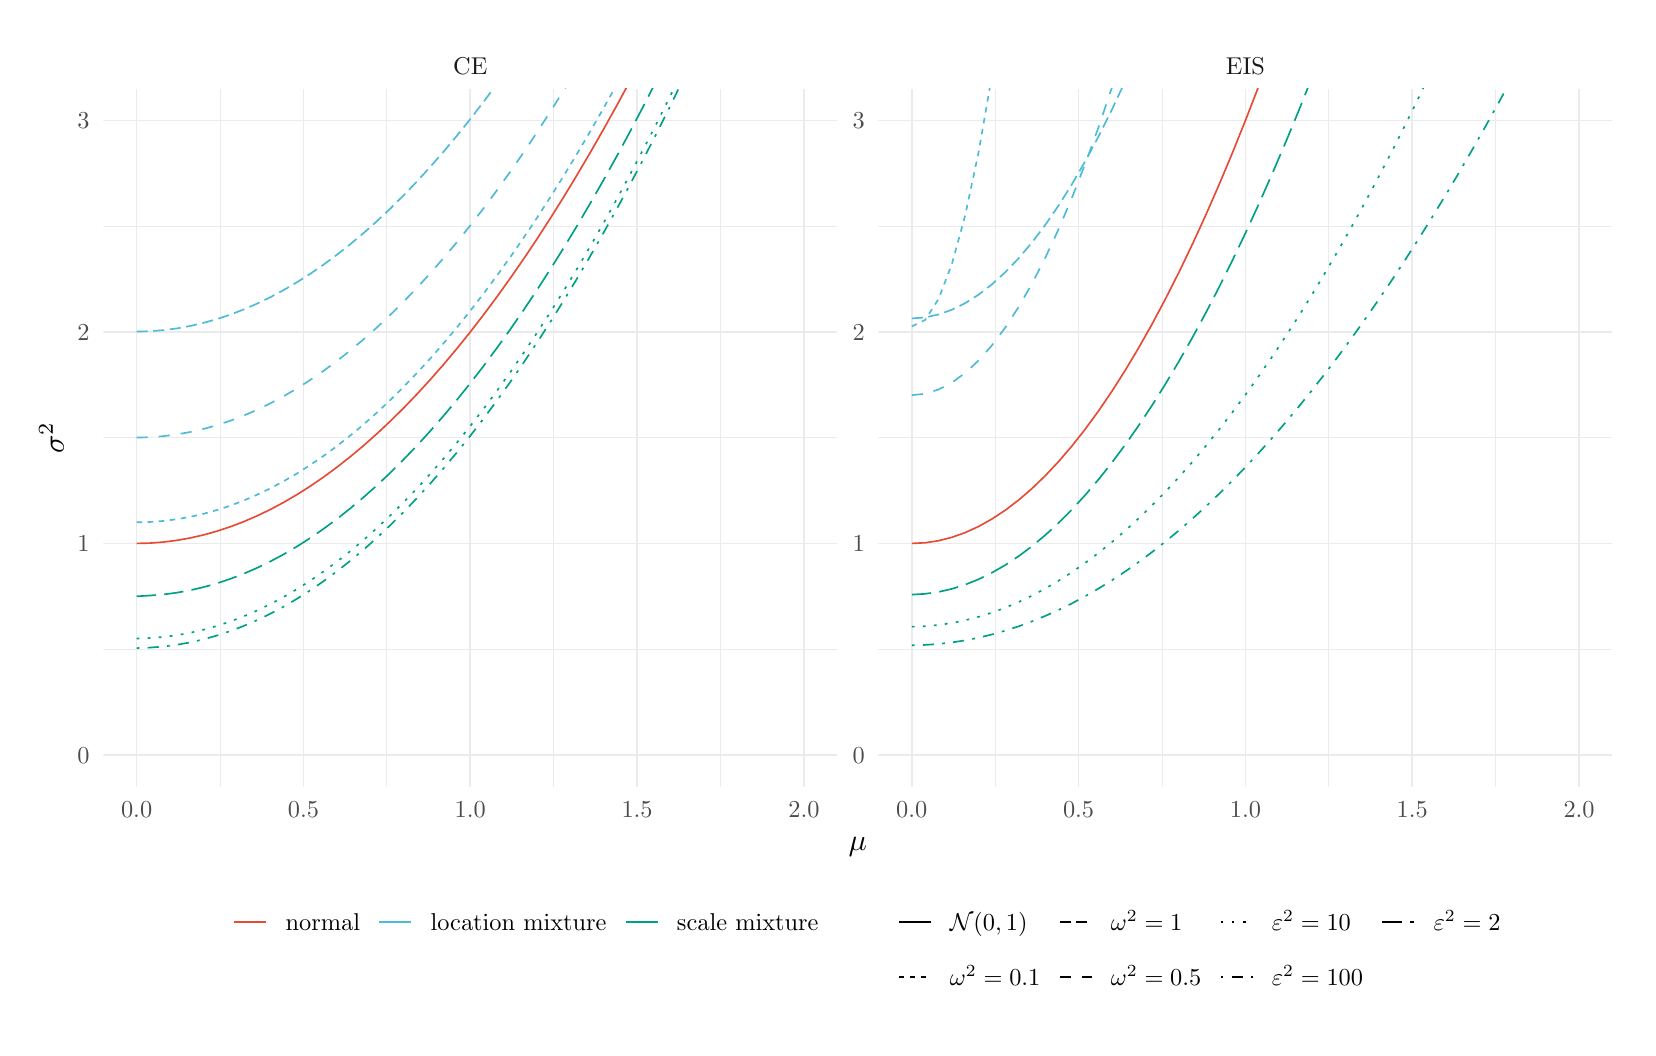
\begin{tikzpicture}[x=1pt,y=1pt]
\definecolor{fillColor}{RGB}{255,255,255}
\path[use as bounding box,fill=fillColor,fill opacity=0.00] (0,0) rectangle (578.16,361.35);
\begin{scope}
\path[clip] ( 27.31, 87.09) rectangle (292.56,339.28);
\definecolor{drawColor}{gray}{0.92}

\path[draw=drawColor,line width= 0.3pt,line join=round] ( 27.31,136.77) --
	(292.56,136.77);

\path[draw=drawColor,line width= 0.3pt,line join=round] ( 27.31,213.19) --
	(292.56,213.19);

\path[draw=drawColor,line width= 0.3pt,line join=round] ( 27.31,289.61) --
	(292.56,289.61);

\path[draw=drawColor,line width= 0.3pt,line join=round] ( 69.51, 87.09) --
	( 69.51,339.28);

\path[draw=drawColor,line width= 0.3pt,line join=round] (129.80, 87.09) --
	(129.80,339.28);

\path[draw=drawColor,line width= 0.3pt,line join=round] (190.08, 87.09) --
	(190.08,339.28);

\path[draw=drawColor,line width= 0.3pt,line join=round] (250.36, 87.09) --
	(250.36,339.28);

\path[draw=drawColor,line width= 0.6pt,line join=round] ( 27.31, 98.56) --
	(292.56, 98.56);

\path[draw=drawColor,line width= 0.6pt,line join=round] ( 27.31,174.98) --
	(292.56,174.98);

\path[draw=drawColor,line width= 0.6pt,line join=round] ( 27.31,251.40) --
	(292.56,251.40);

\path[draw=drawColor,line width= 0.6pt,line join=round] ( 27.31,327.82) --
	(292.56,327.82);

\path[draw=drawColor,line width= 0.6pt,line join=round] ( 39.37, 87.09) --
	( 39.37,339.28);

\path[draw=drawColor,line width= 0.6pt,line join=round] ( 99.65, 87.09) --
	( 99.65,339.28);

\path[draw=drawColor,line width= 0.6pt,line join=round] (159.94, 87.09) --
	(159.94,339.28);

\path[draw=drawColor,line width= 0.6pt,line join=round] (220.22, 87.09) --
	(220.22,339.28);

\path[draw=drawColor,line width= 0.6pt,line join=round] (280.51, 87.09) --
	(280.51,339.28);
\definecolor{drawColor}{RGB}{230,75,53}

\path[draw=drawColor,line width= 0.6pt,line join=round] ( 39.37,174.98) --
	( 44.19,175.10) --
	( 49.02,175.47) --
	( 53.84,176.08) --
	( 58.66,176.93) --
	( 63.48,178.03) --
	( 68.31,179.38) --
	( 73.13,180.97) --
	( 77.95,182.80) --
	( 82.77,184.88) --
	( 87.60,187.20) --
	( 92.42,189.77) --
	( 97.24,192.58) --
	(102.07,195.64) --
	(106.89,198.94) --
	(111.71,202.49) --
	(116.53,206.28) --
	(121.36,210.31) --
	(126.18,214.59) --
	(131.00,219.12) --
	(135.82,223.88) --
	(140.65,228.90) --
	(145.47,234.16) --
	(150.29,239.66) --
	(155.12,245.40) --
	(159.94,251.40) --
	(164.76,257.63) --
	(169.58,264.11) --
	(174.41,270.84) --
	(179.23,277.81) --
	(184.05,285.02) --
	(188.87,292.48) --
	(193.70,300.18) --
	(198.52,308.13) --
	(203.34,316.32) --
	(208.16,324.76) --
	(212.99,333.44) --
	(217.81,342.37) --
	(222.63,351.54) --
	(227.46,360.95) --
	(232.28,370.61) --
	(237.10,380.51) --
	(241.92,390.66) --
	(246.75,401.06) --
	(251.57,411.69) --
	(256.39,422.58) --
	(261.21,433.70) --
	(266.04,445.07) --
	(270.86,456.69) --
	(275.68,468.55) --
	(280.51,480.65);
\definecolor{drawColor}{RGB}{77,187,213}

\path[draw=drawColor,line width= 0.6pt,dash pattern=on 2pt off 2pt ,line join=round] ( 39.37,182.61) --
	( 44.19,182.73) --
	( 49.02,183.10) --
	( 53.84,183.71) --
	( 58.66,184.57) --
	( 63.48,185.67) --
	( 68.31,187.01) --
	( 73.13,188.60) --
	( 77.95,190.44) --
	( 82.77,192.52) --
	( 87.60,194.84) --
	( 92.42,197.41) --
	( 97.24,200.22) --
	(102.07,203.28) --
	(106.89,206.58) --
	(111.71,210.13) --
	(116.53,213.92) --
	(121.36,217.95) --
	(126.18,222.23) --
	(131.00,226.76) --
	(135.82,231.53) --
	(140.65,236.54) --
	(145.47,241.80) --
	(150.29,247.30) --
	(155.12,253.05) --
	(159.94,259.04) --
	(164.76,265.27) --
	(169.58,271.76) --
	(174.41,278.48) --
	(179.23,285.45) --
	(184.05,292.66) --
	(188.87,300.12) --
	(193.70,307.83) --
	(198.52,315.78) --
	(203.34,323.97) --
	(208.16,332.40) --
	(212.99,341.09) --
	(217.81,350.01) --
	(222.63,359.18) --
	(227.46,368.60) --
	(232.28,378.26) --
	(237.10,388.16) --
	(241.92,398.31) --
	(246.75,408.70) --
	(251.57,419.34) --
	(256.39,430.23) --
	(261.21,441.35) --
	(266.04,452.72) --
	(270.86,464.34) --
	(275.68,476.20) --
	(280.51,488.31);

\path[draw=drawColor,line width= 0.6pt,dash pattern=on 4pt off 2pt ,line join=round] ( 39.37,251.53) --
	( 44.19,251.66) --
	( 49.02,252.04) --
	( 53.84,252.67) --
	( 58.66,253.54) --
	( 63.48,254.66) --
	( 68.31,256.02) --
	( 73.13,257.62) --
	( 77.95,259.47) --
	( 82.77,261.57) --
	( 87.60,263.90) --
	( 92.42,266.49) --
	( 97.24,269.31) --
	(102.07,272.39) --
	(106.89,275.70) --
	(111.71,279.26) --
	(116.53,283.07) --
	(121.36,287.12) --
	(126.18,291.41) --
	(131.00,295.95) --
	(135.82,300.74) --
	(140.65,305.76) --
	(145.47,311.04) --
	(150.29,316.55) --
	(155.12,322.32) --
	(159.94,328.32) --
	(164.76,334.57) --
	(169.58,341.07) --
	(174.41,347.81) --
	(179.23,354.79) --
	(184.05,362.02) --
	(188.87,369.50) --
	(193.70,377.22) --
	(198.52,385.18) --
	(203.34,393.39) --
	(208.16,401.84) --
	(212.99,410.53) --
	(217.81,419.47) --
	(222.63,428.66) --
	(227.46,438.09) --
	(232.28,447.76) --
	(237.10,457.68) --
	(241.92,467.85) --
	(246.75,478.26) --
	(251.57,488.91) --
	(256.39,499.81) --
	(261.21,510.95) --
	(266.04,522.33) --
	(270.86,533.96) --
	(275.68,545.84) --
	(280.51,557.96);

\path[draw=drawColor,line width= 0.6pt,dash pattern=on 4pt off 4pt ,line join=round] ( 39.37,213.23) --
	( 44.19,213.36) --
	( 49.02,213.74) --
	( 53.84,214.36) --
	( 58.66,215.22) --
	( 63.48,216.33) --
	( 68.31,217.68) --
	( 73.13,219.28) --
	( 77.95,221.13) --
	( 82.77,223.21) --
	( 87.60,225.55) --
	( 92.42,228.12) --
	( 97.24,230.94) --
	(102.07,234.01) --
	(106.89,237.32) --
	(111.71,240.87) --
	(116.53,244.67) --
	(121.36,248.72) --
	(126.18,253.00) --
	(131.00,257.54) --
	(135.82,262.31) --
	(140.65,267.34) --
	(145.47,272.60) --
	(150.29,278.11) --
	(155.12,283.87) --
	(159.94,289.87) --
	(164.76,296.11) --
	(169.58,302.60) --
	(174.41,309.34) --
	(179.23,316.32) --
	(184.05,323.54) --
	(188.87,331.01) --
	(193.70,338.72) --
	(198.52,346.67) --
	(203.34,354.88) --
	(208.16,363.32) --
	(212.99,372.01) --
	(217.81,380.95) --
	(222.63,390.12) --
	(227.46,399.55) --
	(232.28,409.22) --
	(237.10,419.13) --
	(241.92,429.29) --
	(246.75,439.69) --
	(251.57,450.33) --
	(256.39,461.23) --
	(261.21,472.36) --
	(266.04,483.74) --
	(270.86,495.37) --
	(275.68,507.24) --
	(280.51,519.35);
\definecolor{drawColor}{RGB}{0,160,135}

\path[draw=drawColor,line width= 0.6pt,dash pattern=on 1pt off 3pt ,line join=round] ( 39.37,140.59) --
	( 44.19,140.80) --
	( 49.02,141.18) --
	( 53.84,141.80) --
	( 58.66,142.67) --
	( 63.48,143.78) --
	( 68.31,145.14) --
	( 73.13,146.74) --
	( 77.95,148.59) --
	( 82.77,150.68) --
	( 87.60,153.02) --
	( 92.42,155.60) --
	( 97.24,158.42) --
	(102.07,161.49) --
	(106.89,164.81) --
	(111.71,168.36) --
	(116.53,172.17) --
	(121.36,176.22) --
	(126.18,180.51) --
	(131.00,185.05) --
	(135.82,189.83) --
	(140.65,194.85) --
	(145.47,200.12) --
	(150.29,205.64) --
	(155.12,211.40) --
	(159.94,217.40) --
	(164.76,223.65) --
	(169.58,230.14) --
	(174.41,236.88) --
	(179.23,243.86) --
	(184.05,251.09) --
	(188.87,258.56) --
	(193.70,266.28) --
	(198.52,274.24) --
	(203.34,282.44) --
	(208.16,290.89) --
	(212.99,299.59) --
	(217.81,308.53) --
	(222.63,317.71) --
	(227.46,327.14) --
	(232.28,336.81) --
	(237.10,346.73) --
	(241.92,356.89) --
	(246.75,367.29) --
	(251.57,377.94) --
	(256.39,388.84) --
	(261.21,399.98) --
	(266.04,411.36) --
	(270.86,422.99) --
	(275.68,434.86) --
	(280.51,446.98);

\path[draw=drawColor,line width= 0.6pt,dash pattern=on 1pt off 3pt on 4pt off 3pt ,line join=round] ( 39.37,137.15) --
	( 44.19,137.34) --
	( 49.02,137.72) --
	( 53.84,138.34) --
	( 58.66,139.20) --
	( 63.48,140.31) --
	( 68.31,141.67) --
	( 73.13,143.27) --
	( 77.95,145.11) --
	( 82.77,147.20) --
	( 87.60,149.53) --
	( 92.42,152.11) --
	( 97.24,154.93) --
	(102.07,158.00) --
	(106.89,161.31) --
	(111.71,164.87) --
	(116.53,168.67) --
	(121.36,172.71) --
	(126.18,177.00) --
	(131.00,181.54) --
	(135.82,186.32) --
	(140.65,191.34) --
	(145.47,196.61) --
	(150.29,202.12) --
	(155.12,207.88) --
	(159.94,213.88) --
	(164.76,220.12) --
	(169.58,226.62) --
	(174.41,233.35) --
	(179.23,240.33) --
	(184.05,247.55) --
	(188.87,255.02) --
	(193.70,262.74) --
	(198.52,270.69) --
	(203.34,278.90) --
	(208.16,287.34) --
	(212.99,296.03) --
	(217.81,304.97) --
	(222.63,314.15) --
	(227.46,323.58) --
	(232.28,333.24) --
	(237.10,343.16) --
	(241.92,353.32) --
	(246.75,363.72) --
	(251.57,374.37) --
	(256.39,385.26) --
	(261.21,396.40) --
	(266.04,407.78) --
	(270.86,419.40) --
	(275.68,431.28) --
	(280.51,443.39);

\path[draw=drawColor,line width= 0.6pt,dash pattern=on 7pt off 3pt ,line join=round] ( 39.37,155.87) --
	( 44.19,156.15) --
	( 49.02,156.54) --
	( 53.84,157.17) --
	( 58.66,158.04) --
	( 63.48,159.16) --
	( 68.31,160.52) --
	( 73.13,162.13) --
	( 77.95,163.98) --
	( 82.77,166.08) --
	( 87.60,168.42) --
	( 92.42,171.00) --
	( 97.24,173.83) --
	(102.07,176.91) --
	(106.89,180.23) --
	(111.71,183.79) --
	(116.53,187.60) --
	(121.36,191.65) --
	(126.18,195.95) --
	(131.00,200.49) --
	(135.82,205.28) --
	(140.65,210.31) --
	(145.47,215.59) --
	(150.29,221.11) --
	(155.12,226.87) --
	(159.94,232.88) --
	(164.76,239.13) --
	(169.58,245.63) --
	(174.41,252.37) --
	(179.23,259.36) --
	(184.05,266.59) --
	(188.87,274.07) --
	(193.70,281.79) --
	(198.52,289.76) --
	(203.34,297.97) --
	(208.16,306.42) --
	(212.99,315.12) --
	(217.81,324.06) --
	(222.63,333.25) --
	(227.46,342.69) --
	(232.28,352.36) --
	(237.10,362.28) --
	(241.92,372.45) --
	(246.75,382.86) --
	(251.57,393.52) --
	(256.39,404.42) --
	(261.21,415.56) --
	(266.04,426.95) --
	(270.86,438.58) --
	(275.68,450.46) --
	(280.51,462.59);
\end{scope}
\begin{scope}
\path[clip] (307.41, 87.09) rectangle (572.66,339.28);
\definecolor{drawColor}{gray}{0.92}

\path[draw=drawColor,line width= 0.3pt,line join=round] (307.41,136.77) --
	(572.66,136.77);

\path[draw=drawColor,line width= 0.3pt,line join=round] (307.41,213.19) --
	(572.66,213.19);

\path[draw=drawColor,line width= 0.3pt,line join=round] (307.41,289.61) --
	(572.66,289.61);

\path[draw=drawColor,line width= 0.3pt,line join=round] (349.61, 87.09) --
	(349.61,339.28);

\path[draw=drawColor,line width= 0.3pt,line join=round] (409.89, 87.09) --
	(409.89,339.28);

\path[draw=drawColor,line width= 0.3pt,line join=round] (470.18, 87.09) --
	(470.18,339.28);

\path[draw=drawColor,line width= 0.3pt,line join=round] (530.46, 87.09) --
	(530.46,339.28);

\path[draw=drawColor,line width= 0.6pt,line join=round] (307.41, 98.56) --
	(572.66, 98.56);

\path[draw=drawColor,line width= 0.6pt,line join=round] (307.41,174.98) --
	(572.66,174.98);

\path[draw=drawColor,line width= 0.6pt,line join=round] (307.41,251.40) --
	(572.66,251.40);

\path[draw=drawColor,line width= 0.6pt,line join=round] (307.41,327.82) --
	(572.66,327.82);

\path[draw=drawColor,line width= 0.6pt,line join=round] (319.47, 87.09) --
	(319.47,339.28);

\path[draw=drawColor,line width= 0.6pt,line join=round] (379.75, 87.09) --
	(379.75,339.28);

\path[draw=drawColor,line width= 0.6pt,line join=round] (440.04, 87.09) --
	(440.04,339.28);

\path[draw=drawColor,line width= 0.6pt,line join=round] (500.32, 87.09) --
	(500.32,339.28);

\path[draw=drawColor,line width= 0.6pt,line join=round] (560.60, 87.09) --
	(560.60,339.28);
\definecolor{drawColor}{RGB}{230,75,53}

\path[draw=drawColor,line width= 0.6pt,line join=round] (319.47,174.98) --
	(324.29,175.22) --
	(329.11,175.95) --
	(333.94,177.18) --
	(338.76,178.89) --
	(343.58,181.09) --
	(348.40,183.78) --
	(353.23,186.96) --
	(358.05,190.63) --
	(362.87,194.78) --
	(367.69,199.43) --
	(372.52,204.57) --
	(377.34,210.19) --
	(382.16,216.30) --
	(386.99,222.91) --
	(391.81,230.00) --
	(396.63,237.58) --
	(401.45,245.65) --
	(406.28,254.21) --
	(411.10,263.26) --
	(415.92,272.79) --
	(420.74,282.82) --
	(425.57,293.34) --
	(430.39,304.34) --
	(435.21,315.83) --
	(440.04,327.82) --
	(444.86,340.29) --
	(449.68,353.25) --
	(454.50,366.70) --
	(459.33,380.64) --
	(464.15,395.06) --
	(468.97,409.98) --
	(473.79,425.39) --
	(478.62,441.28) --
	(483.44,457.67) --
	(488.26,474.54) --
	(493.09,491.90) --
	(497.91,509.76) --
	(502.73,528.10) --
	(507.55,546.93) --
	(512.38,566.24) --
	(517.20,586.05) --
	(522.02,606.35) --
	(526.84,627.14) --
	(531.67,648.41) --
	(536.49,670.18) --
	(541.31,692.43) --
	(546.14,715.17) --
	(550.96,738.40) --
	(555.78,762.12) --
	(560.60,786.33);
\definecolor{drawColor}{RGB}{77,187,213}

\path[draw=drawColor,line width= 0.6pt,dash pattern=on 2pt off 2pt ,line join=round] (319.47,253.37) --
	(324.29,255.74) --
	(329.11,263.25) --
	(333.94,275.85) --
	(338.76,293.50) --
	(343.58,316.21) --
	(348.40,343.89) --
	(353.23,376.55) --
	(358.05,414.12) --
	(362.87,456.58) --
	(367.69,503.89) --
	(372.52,556.02) --
	(377.34,612.95) --
	(382.16,674.67) --
	(386.99,741.02) --
	(391.81,812.14) --
	(396.63,887.86) --
	(401.45,968.22) --
	(406.28,1053.15) --
	(411.10,1142.72) --
	(415.92,1236.78) --
	(420.74,1335.35) --
	(425.57,1438.31) --
	(430.39,1545.87) --
	(435.21,1657.71) --
	(440.04,1773.94) --
	(444.86,1894.45) --
	(449.68,2019.33) --
	(454.50,2149.01) --
	(459.33,2282.57) --
	(464.15,2420.09) --
	(468.97,2562.24) --
	(472.67,2673.99);

\path[draw=drawColor,line width= 0.6pt,dash pattern=on 4pt off 2pt ,line join=round] (319.47,256.27) --
	(324.29,256.65) --
	(329.11,257.70) --
	(333.94,259.42) --
	(338.76,261.80) --
	(343.58,264.85) --
	(348.40,268.56) --
	(353.23,272.94) --
	(358.05,277.98) --
	(362.87,283.68) --
	(367.69,290.05) --
	(372.52,297.08) --
	(377.34,304.77) --
	(382.16,313.11) --
	(386.99,322.12) --
	(391.81,331.79) --
	(396.63,342.12) --
	(401.45,353.10) --
	(406.28,364.74) --
	(411.10,377.04) --
	(415.92,389.99) --
	(420.74,403.59) --
	(425.57,417.85) --
	(430.39,432.76) --
	(435.21,448.32) --
	(440.04,464.53) --
	(444.86,481.40) --
	(449.68,498.91) --
	(454.50,517.07) --
	(459.33,535.88) --
	(464.15,555.33) --
	(468.97,575.44) --
	(473.79,596.19) --
	(478.62,617.61) --
	(483.44,639.64) --
	(488.26,662.32) --
	(493.09,685.68) --
	(497.91,709.64) --
	(502.73,734.25) --
	(507.55,759.50) --
	(512.38,785.43) --
	(517.20,811.96) --
	(522.02,839.13) --
	(526.84,866.96) --
	(531.67,895.44) --
	(536.49,924.52) --
	(541.31,954.24) --
	(546.14,984.62) --
	(550.96,1015.61) --
	(555.78,1047.23) --
	(560.60,1079.50);

\path[draw=drawColor,line width= 0.6pt,dash pattern=on 4pt off 4pt ,line join=round] (319.47,228.55) --
	(324.29,229.07) --
	(329.11,230.58) --
	(333.94,233.08) --
	(338.76,236.57) --
	(343.58,241.05) --
	(348.40,246.51) --
	(353.23,252.95) --
	(358.05,260.38) --
	(362.87,268.79) --
	(367.69,278.18) --
	(372.52,288.55) --
	(377.34,299.89) --
	(382.16,312.21) --
	(386.99,325.51) --
	(391.81,339.77) --
	(396.63,355.01) --
	(401.45,371.21) --
	(406.28,388.38) --
	(411.10,406.52) --
	(415.92,425.62) --
	(420.74,445.70) --
	(425.57,466.71) --
	(430.39,488.70) --
	(435.21,511.65) --
	(440.04,535.55) --
	(444.86,560.41) --
	(449.68,586.21) --
	(454.50,612.97) --
	(459.33,640.69) --
	(464.15,669.32) --
	(468.97,699.01) --
	(473.79,729.54) --
	(478.62,761.07) --
	(483.44,793.48) --
	(488.26,826.91) --
	(493.09,861.17) --
	(497.91,896.51) --
	(502.73,932.63) --
	(507.55,969.87) --
	(512.38,1007.97) --
	(517.20,1046.99) --
	(522.02,1086.95) --
	(526.84,1127.81) --
	(531.67,1169.63) --
	(536.49,1212.38) --
	(541.31,1256.07) --
	(546.14,1300.60) --
	(550.96,1346.15) --
	(555.78,1392.61) --
	(560.60,1440.03);
\definecolor{drawColor}{RGB}{0,160,135}

\path[draw=drawColor,line width= 0.6pt,dash pattern=on 1pt off 3pt ,line join=round] (319.47,144.89) --
	(324.29,145.06) --
	(329.11,145.51) --
	(333.94,146.22) --
	(338.76,147.20) --
	(343.58,148.44) --
	(348.40,149.96) --
	(353.23,151.73) --
	(358.05,153.78) --
	(362.87,156.09) --
	(367.69,158.66) --
	(372.52,161.50) --
	(377.34,164.60) --
	(382.16,167.97) --
	(386.99,171.59) --
	(391.81,175.48) --
	(396.63,179.63) --
	(401.45,184.05) --
	(406.28,188.72) --
	(411.10,193.65) --
	(415.92,198.85) --
	(420.74,204.30) --
	(425.57,210.01) --
	(430.39,215.98) --
	(435.21,222.21) --
	(440.04,228.70) --
	(444.86,235.44) --
	(449.68,242.44) --
	(454.50,249.70) --
	(459.33,257.21) --
	(464.15,264.98) --
	(468.97,273.00) --
	(473.79,281.28) --
	(478.62,289.81) --
	(483.44,298.59) --
	(488.26,307.63) --
	(493.09,316.92) --
	(497.91,326.46) --
	(502.73,336.26) --
	(507.55,346.30) --
	(512.38,356.60) --
	(517.20,367.15) --
	(522.02,377.95) --
	(526.84,388.99) --
	(531.67,400.29) --
	(536.49,411.84) --
	(541.31,423.63) --
	(546.14,435.67) --
	(550.96,447.94) --
	(555.78,460.49) --
	(560.60,473.29);

\path[draw=drawColor,line width= 0.6pt,dash pattern=on 1pt off 3pt on 4pt off 3pt ,line join=round] (319.47,138.17) --
	(324.29,138.31) --
	(329.11,138.65) --
	(333.94,139.20) --
	(338.76,139.95) --
	(343.58,140.91) --
	(348.40,142.07) --
	(353.23,143.44) --
	(358.05,145.01) --
	(362.87,146.79) --
	(367.69,148.77) --
	(372.52,150.94) --
	(377.34,153.32) --
	(382.16,155.91) --
	(386.99,158.69) --
	(391.81,161.68) --
	(396.63,164.86) --
	(401.45,168.25) --
	(406.28,171.84) --
	(411.10,175.62) --
	(415.92,179.61) --
	(420.74,183.80) --
	(425.57,188.18) --
	(430.39,192.77) --
	(435.21,197.55) --
	(440.04,202.53) --
	(444.86,207.71) --
	(449.68,213.09) --
	(454.50,218.66) --
	(459.33,224.43) --
	(464.15,230.41) --
	(468.97,236.57) --
	(473.79,242.93) --
	(478.62,249.49) --
	(483.44,256.25) --
	(488.26,263.19) --
	(493.09,270.33) --
	(497.91,277.68) --
	(502.73,285.21) --
	(507.55,292.94) --
	(512.38,300.86) --
	(517.20,308.97) --
	(522.02,317.29) --
	(526.84,325.79) --
	(531.67,334.49) --
	(536.49,343.38) --
	(541.31,352.45) --
	(546.14,361.73) --
	(550.96,371.19) --
	(555.78,380.85) --
	(560.60,390.70);

\path[draw=drawColor,line width= 0.6pt,dash pattern=on 7pt off 3pt ,line join=round] (319.47,156.49) --
	(324.29,156.76) --
	(329.11,157.44) --
	(333.94,158.55) --
	(338.76,160.07) --
	(343.58,162.02) --
	(348.40,164.38) --
	(353.23,167.15) --
	(358.05,170.34) --
	(362.87,173.95) --
	(367.69,177.96) --
	(372.52,182.39) --
	(377.34,187.23) --
	(382.16,192.48) --
	(386.99,198.14) --
	(391.81,204.21) --
	(396.63,210.68) --
	(401.45,217.56) --
	(406.28,224.85) --
	(411.10,232.54) --
	(415.92,240.63) --
	(420.74,249.13) --
	(425.57,258.02) --
	(430.39,267.32) --
	(435.21,277.01) --
	(440.04,287.11) --
	(444.86,297.60) --
	(449.68,308.49) --
	(454.50,319.77) --
	(459.33,331.45) --
	(464.15,343.52) --
	(468.97,355.99) --
	(473.79,368.84) --
	(478.62,382.09) --
	(483.44,395.73) --
	(488.26,409.75) --
	(493.09,424.17) --
	(497.91,438.97) --
	(502.73,454.15) --
	(507.55,469.73) --
	(512.38,485.70) --
	(517.20,502.03) --
	(522.02,518.76) --
	(526.84,535.86) --
	(531.67,553.34) --
	(536.49,571.22) --
	(541.31,589.48) --
	(546.14,608.07) --
	(550.96,627.10) --
	(555.78,646.47) --
	(560.60,666.22);
\end{scope}
\begin{scope}
\path[clip] ( 27.31,339.28) rectangle (292.56,355.85);
\definecolor{drawColor}{gray}{0.10}

\node[text=drawColor,anchor=base,inner sep=0pt, outer sep=0pt, scale=  0.88] at (159.94,344.53) {CE};
\end{scope}
\begin{scope}
\path[clip] (307.41,339.28) rectangle (572.66,355.85);
\definecolor{drawColor}{gray}{0.10}

\node[text=drawColor,anchor=base,inner sep=0pt, outer sep=0pt, scale=  0.88] at (440.04,344.53) {EIS};
\end{scope}
\begin{scope}
\path[clip] (  0.00,  0.00) rectangle (578.16,361.35);
\definecolor{drawColor}{gray}{0.30}

\node[text=drawColor,anchor=base,inner sep=0pt, outer sep=0pt, scale=  0.88] at ( 39.37, 76.08) {0.0};

\node[text=drawColor,anchor=base,inner sep=0pt, outer sep=0pt, scale=  0.88] at ( 99.65, 76.08) {0.5};

\node[text=drawColor,anchor=base,inner sep=0pt, outer sep=0pt, scale=  0.88] at (159.94, 76.08) {1.0};

\node[text=drawColor,anchor=base,inner sep=0pt, outer sep=0pt, scale=  0.88] at (220.22, 76.08) {1.5};

\node[text=drawColor,anchor=base,inner sep=0pt, outer sep=0pt, scale=  0.88] at (280.51, 76.08) {2.0};
\end{scope}
\begin{scope}
\path[clip] (  0.00,  0.00) rectangle (578.16,361.35);
\definecolor{drawColor}{gray}{0.30}

\node[text=drawColor,anchor=base,inner sep=0pt, outer sep=0pt, scale=  0.88] at (319.47, 76.08) {0.0};

\node[text=drawColor,anchor=base,inner sep=0pt, outer sep=0pt, scale=  0.88] at (379.75, 76.08) {0.5};

\node[text=drawColor,anchor=base,inner sep=0pt, outer sep=0pt, scale=  0.88] at (440.04, 76.08) {1.0};

\node[text=drawColor,anchor=base,inner sep=0pt, outer sep=0pt, scale=  0.88] at (500.32, 76.08) {1.5};

\node[text=drawColor,anchor=base,inner sep=0pt, outer sep=0pt, scale=  0.88] at (560.60, 76.08) {2.0};
\end{scope}
\begin{scope}
\path[clip] (  0.00,  0.00) rectangle (578.16,361.35);
\definecolor{drawColor}{gray}{0.30}

\node[text=drawColor,anchor=base east,inner sep=0pt, outer sep=0pt, scale=  0.88] at (302.46, 95.53) {0};

\node[text=drawColor,anchor=base east,inner sep=0pt, outer sep=0pt, scale=  0.88] at (302.46,171.95) {1};

\node[text=drawColor,anchor=base east,inner sep=0pt, outer sep=0pt, scale=  0.88] at (302.46,248.37) {2};

\node[text=drawColor,anchor=base east,inner sep=0pt, outer sep=0pt, scale=  0.88] at (302.46,324.79) {3};
\end{scope}
\begin{scope}
\path[clip] (  0.00,  0.00) rectangle (578.16,361.35);
\definecolor{drawColor}{gray}{0.30}

\node[text=drawColor,anchor=base east,inner sep=0pt, outer sep=0pt, scale=  0.88] at ( 22.36, 95.53) {0};

\node[text=drawColor,anchor=base east,inner sep=0pt, outer sep=0pt, scale=  0.88] at ( 22.36,171.95) {1};

\node[text=drawColor,anchor=base east,inner sep=0pt, outer sep=0pt, scale=  0.88] at ( 22.36,248.37) {2};

\node[text=drawColor,anchor=base east,inner sep=0pt, outer sep=0pt, scale=  0.88] at ( 22.36,324.79) {3};
\end{scope}
\begin{scope}
\path[clip] (  0.00,  0.00) rectangle (578.16,361.35);
\definecolor{drawColor}{RGB}{0,0,0}

\node[text=drawColor,anchor=base,inner sep=0pt, outer sep=0pt, scale=  1.10] at (299.99, 64.05) {$\mu$};
\end{scope}
\begin{scope}
\path[clip] (  0.00,  0.00) rectangle (578.16,361.35);
\definecolor{drawColor}{RGB}{0,0,0}

\node[text=drawColor,rotate= 90.00,anchor=base,inner sep=0pt, outer sep=0pt, scale=  1.10] at ( 13.08,213.19) {$\sigma^2$};
\end{scope}
\begin{scope}
\path[clip] (  0.00,  0.00) rectangle (578.16,361.35);
\definecolor{drawColor}{RGB}{230,75,53}

\path[draw=drawColor,line width= 0.6pt,line join=round] ( 74.73, 38.18) -- ( 86.29, 38.18);
\end{scope}
\begin{scope}
\path[clip] (  0.00,  0.00) rectangle (578.16,361.35);
\definecolor{drawColor}{RGB}{77,187,213}

\path[draw=drawColor,line width= 0.6pt,line join=round] (127.09, 38.18) -- (138.65, 38.18);
\end{scope}
\begin{scope}
\path[clip] (  0.00,  0.00) rectangle (578.16,361.35);
\definecolor{drawColor}{RGB}{0,160,135}

\path[draw=drawColor,line width= 0.6pt,line join=round] (216.11, 38.18) -- (227.67, 38.18);
\end{scope}
\begin{scope}
\path[clip] (  0.00,  0.00) rectangle (578.16,361.35);
\definecolor{drawColor}{RGB}{0,0,0}

\node[text=drawColor,anchor=base west,inner sep=0pt, outer sep=0pt, scale=  0.88] at ( 93.24, 35.15) {normal};
\end{scope}
\begin{scope}
\path[clip] (  0.00,  0.00) rectangle (578.16,361.35);
\definecolor{drawColor}{RGB}{0,0,0}

\node[text=drawColor,anchor=base west,inner sep=0pt, outer sep=0pt, scale=  0.88] at (145.60, 35.15) {location mixture};
\end{scope}
\begin{scope}
\path[clip] (  0.00,  0.00) rectangle (578.16,361.35);
\definecolor{drawColor}{RGB}{0,0,0}

\node[text=drawColor,anchor=base west,inner sep=0pt, outer sep=0pt, scale=  0.88] at (234.62, 35.15) {scale mixture};
\end{scope}
\begin{scope}
\path[clip] (  0.00,  0.00) rectangle (578.16,361.35);
\definecolor{drawColor}{RGB}{0,0,0}

\path[draw=drawColor,line width= 0.6pt,line join=round] (314.71, 38.18) -- (326.28, 38.18);
\end{scope}
\begin{scope}
\path[clip] (  0.00,  0.00) rectangle (578.16,361.35);
\definecolor{drawColor}{RGB}{0,0,0}

\path[draw=drawColor,line width= 0.6pt,dash pattern=on 2pt off 2pt ,line join=round] (314.71, 18.23) -- (326.28, 18.23);
\end{scope}
\begin{scope}
\path[clip] (  0.00,  0.00) rectangle (578.16,361.35);
\definecolor{drawColor}{RGB}{0,0,0}

\path[draw=drawColor,line width= 0.6pt,dash pattern=on 4pt off 2pt ,line join=round] (372.89, 38.18) -- (384.45, 38.18);
\end{scope}
\begin{scope}
\path[clip] (  0.00,  0.00) rectangle (578.16,361.35);
\definecolor{drawColor}{RGB}{0,0,0}

\path[draw=drawColor,line width= 0.6pt,dash pattern=on 4pt off 4pt ,line join=round] (372.89, 18.23) -- (384.45, 18.23);
\end{scope}
\begin{scope}
\path[clip] (  0.00,  0.00) rectangle (578.16,361.35);
\definecolor{drawColor}{RGB}{0,0,0}

\path[draw=drawColor,line width= 0.6pt,dash pattern=on 1pt off 3pt ,line join=round] (431.06, 38.18) -- (442.62, 38.18);
\end{scope}
\begin{scope}
\path[clip] (  0.00,  0.00) rectangle (578.16,361.35);
\definecolor{drawColor}{RGB}{0,0,0}

\path[draw=drawColor,line width= 0.6pt,dash pattern=on 1pt off 3pt on 4pt off 3pt ,line join=round] (431.06, 18.23) -- (442.62, 18.23);
\end{scope}
\begin{scope}
\path[clip] (  0.00,  0.00) rectangle (578.16,361.35);
\definecolor{drawColor}{RGB}{0,0,0}

\path[draw=drawColor,line width= 0.6pt,dash pattern=on 7pt off 3pt ,line join=round] (489.50, 38.18) -- (501.06, 38.18);
\end{scope}
\begin{scope}
\path[clip] (  0.00,  0.00) rectangle (578.16,361.35);
\definecolor{drawColor}{RGB}{0,0,0}

\node[text=drawColor,anchor=base west,inner sep=0pt, outer sep=0pt, scale=  0.88] at (333.22, 35.15) {$\mathcal N (0, 1)$};
\end{scope}
\begin{scope}
\path[clip] (  0.00,  0.00) rectangle (578.16,361.35);
\definecolor{drawColor}{RGB}{0,0,0}

\node[text=drawColor,anchor=base west,inner sep=0pt, outer sep=0pt, scale=  0.88] at (333.22, 15.20) {$\omega^2 = 0.1$};
\end{scope}
\begin{scope}
\path[clip] (  0.00,  0.00) rectangle (578.16,361.35);
\definecolor{drawColor}{RGB}{0,0,0}

\node[text=drawColor,anchor=base west,inner sep=0pt, outer sep=0pt, scale=  0.88] at (391.39, 35.15) {$\omega^2 = 1$};
\end{scope}
\begin{scope}
\path[clip] (  0.00,  0.00) rectangle (578.16,361.35);
\definecolor{drawColor}{RGB}{0,0,0}

\node[text=drawColor,anchor=base west,inner sep=0pt, outer sep=0pt, scale=  0.88] at (391.39, 15.20) {$\omega^2= 0.5$};
\end{scope}
\begin{scope}
\path[clip] (  0.00,  0.00) rectangle (578.16,361.35);
\definecolor{drawColor}{RGB}{0,0,0}

\node[text=drawColor,anchor=base west,inner sep=0pt, outer sep=0pt, scale=  0.88] at (449.57, 35.15) {$\varepsilon^2 = 10$};
\end{scope}
\begin{scope}
\path[clip] (  0.00,  0.00) rectangle (578.16,361.35);
\definecolor{drawColor}{RGB}{0,0,0}

\node[text=drawColor,anchor=base west,inner sep=0pt, outer sep=0pt, scale=  0.88] at (449.57, 15.20) {$\varepsilon^2 = 100$};
\end{scope}
\begin{scope}
\path[clip] (  0.00,  0.00) rectangle (578.16,361.35);
\definecolor{drawColor}{RGB}{0,0,0}

\node[text=drawColor,anchor=base west,inner sep=0pt, outer sep=0pt, scale=  0.88] at (508.01, 35.15) {$\varepsilon^2 = 2$};
\end{scope}
\end{tikzpicture}
%
    }
    \caption{{\color{red} TODO}}
    \label{fig:cem_eis_sigma2}
\end{figure}

% AREs
On the left-hand side of \Cref{fig:are} we see that for $\mu$ close to the optimal value, \aeis has smaller asymptotic variance than the \acem, except for the two bimodal location measures. Again, due to the finite sample convergence of \aeis, \Cref{prop:eis-finite-sample}, the asymptotic variance $V_{\eis}$ goes to $0$ as $\mu \to 0$. The more $\mu$ becomes misspecified, the ratio of asymptotic variances starts to grow. 

% sigma2s
In \Cref{fig:cem_eis_sigma2} we see that, except for the extreme scale mixtures, \aeis tends to produce proposals that have a larger variance than those produced by the \acem. As we will see in the discussion of \Cref{fig:rho_mu}, this might be advantageous for \aeis as proposals with a small variance run the risk of missing a large part of the probability mass of the target. \todo{clean this}

In applications, e.g. the model studied in \Cref{cha:analysis_of_selected_models}, we are interested in the performance of the importance sampling proposals generated by the \gls{la}, \gls{cem} and \gls{eis} under more complex circumstances than those discussed in \Cref{ex:univ-gaussian-mu-fixed,ex:univ-gaussian-s2-fixed}. In particular, the dimension of $\psi$ is high ($\mathcal O(n \cdot m)$ or even $\mathcal O(n \cdot m^{2})$) and proposals may not come from a natural exponential family, so analysis based on \Cref{thm:ce-clt,thm:clt-eis} is not possible. Instead, we resort to simulation studies to gain insights into the circumstances when one should prefer one method over the other.
As a leading example, we will use the following vector-autoregressive state space model with negative binomial observations. A similar, though more involved, model is studied in \Cref{sec:regional_growth_factor_model} with real data.

\begin{example}[Negative Binomial $\operatorname{VAR}(1)$ \gls{ssm}]
    \label{ex:negbinom-ar1}
    % setup 
    In this example, we consider a \gls{ssm} where states $X_{t}$ follow a stationary Gaussian $\operatorname{VAR}(1)$ process, initialized in its stationary distribution $\mathcal N(0,\Sigma)$ for \acrshort{spd} $\Sigma$. For simplicity let the transition matrices be given by a multiple of the identity, i.e. $A_{t} = \alpha I_{m}$ for all $t$ where $\alpha \in (-1, 1)$ \todo{add I to symbols}. 
    In total, the states are governed by
    \begin{align*}
    X_{0} &\sim \mathcal N(0,\Sigma) \\
    X_{t} &= \alpha X_{t - 1} + \varepsilon_{t}\\
    \varepsilon_t &\iid \mathcal N(0, (1 - \alpha^{2})\Sigma), t = 1, \dots, n
    \end{align*}
    where the $\varepsilon_{1}, \dots, n$ and $X_{0}$ are jointly independent. The observations follow a conditional negative binomial distribution 
    $$
    Y^{i}_{t} | X_{t} \sim \nbinom \left( \exp(X^{i}_{t}), r \right), \phantom{and} i = 1, \dots, p \phantom{and} t = 0, \dots, n
    $$
    and individual observations are conditionally independent given the current state. The parametrization of the negative binomial distribution $\nbinom \left( \mu, r \right)$ is such that the density is
    $$
        p_{\mu, r}(y) = \binom{y + r - 1}{r} \left( \frac{\mu}{r + \mu} \right)^{y} \left( \frac{r}{r + \mu} \right)^{r} \propto_{\mu} \mu^{y} (\mu + r)^{-(r + y)},
    $$
    with expectation $\mu$, variance $\mu + \frac{\mu^{2}}{r}$ and support $\N_{0}$. 
\end{example}

%% simulation study on MSE/Bias/Variance

Our first simulation study concerns the non-asymptotic behavior of the \gls{cem} and \gls{eis} estimators, i.e. finite sample analogs of \Cref{thm:ce-clt,thm:clt-eis}. To this end,
we let $m = 1$ in \Cref{ex:negbinom-ar1} and fix $n$ to \todo{...}. 
We then simulate once from the marginal distribution of $Y$ and perform the \gls{la} to a prespecified precision $\epsilon$ and maximum number of iterations $n_{\text{iter}}$, obtaining a proposal distribution $\G_{\la}$. Using a large number of samples $N_{\text{true}}$ from this proposal we find the optimal $\G_{\ce}$ and $\G_{\eis}$ using the same desired precision and number of iterations as for the \gls{la}. For the remainder of this section, we ignore sampling variation in these proposals and treat them as exact. 

%% posterior marginal means and variances
To determine the non-asymptotic sampling behavior we now perform the above procedure again, using only $N \ll N_{\text{true}}$ many samples for both procedures, obtaining proposals $\hat\P^{N}_{\ce}$ and $\hat \P^{N}_{\eis}$. As the full proposals are Gaussian distributions on $\R^{(n+1)\times m}$, either given as the posterior of a \gls{glssm} (\gls{la}, \gls{eis}) or by a Gaussian Markov process(\gls{cem}), see \Cref{sec:gaussian_importance_sampling_for_state_space_models}. 
This procedure is repeated $M$ times for every sample size $N$ considered, with different initial random seeds, obtaining $\hat\P^{N,i}_{\ce}$ and $\hat \P^{N,i}_{\eis}$ for $i = 1, \dots, M$.

To assess the speed of convergence of the \gls{cem} and \gls{eis} we then estimate the mean squared error of means and variances of the $(n+1) \times m$ univariate marginals as $N$, the number of samples used to obtain $\hpce$ or $\hpeis$, grows. For the true value, we take the univariate means and variances of $\G_{\ce}$ and $\G_{\eis}$ respectively. Additionally, we perform a bias-variance decomposition to see where the estimation error originates. 

More concretely, fix $N$ and denote by $\mu, \sigma^{2} \in \mathbf R^{(n + 1) \cdot m}$ the marginal means and variances of $\G_{\ce}$ ($\G_{\eis}$). 
Let $\hat\mu_{i}, \hat\sigma^{2}_{i}\in\mathbf R^{(n + 1) \cdot m}$ be the marginal means and variances of $\G^{N,i}_{\ce}$ ($\G^{N,i}_{\eis}$) for $i = 1,\dots, M$. 
Now 
$$
\widehat{\text{aMSE}} = \frac{1}{M} \frac{1}{(n + 1)m} \sum_{i = 1}^M \lVert \mu - \hat\mu_{i} \rVert_{2}^2 + \lVert \sigma^{2} - \hat\sigma_{i}^2 \rVert^{2}_{2}
$$
is an estimate of the mean-squared error of $(\mu, \sigma^{2})$, where we divide by $(n+1)m$ to make estimates comparable across models of different dimensions. 

%The $\text{ASE}_{i}$ is of interest to the practitioner as they usually only run a single iteration of the optimal importance sampling procedure. So while a low $\text{AMSE}$ is desirable, the variance of $\text{ASE}$ should also be small in practice, as otherwise several runs of the optimal importance sampling procedure may be required to obtain a good proposal.

In \Cref{fig:mse_bias_var_decomposition} we show the $\widehat{\text{aMSE}}$ for both the \gls{cem} and \gls{eis} for varying values of $N$. As is evident from this Figure, the \gls{cem} consistently has a larger aMSE than \gls{eis}, for all values of $N$. Thus the \gls{cem} requires several orders of magnitude more samples to obtain the same precision as \gls{eis}.

For further investigation, we perform a bias-variance decomposition of the aMSE for both the means $\mu$ and variances $\sigma^{2}$. Consider the average means and variances over the $M$ simulations,
\begin{align*}
    \bar \mu = \frac{1}{M} \sum_{i=1}^{M} \hat\mu_{i} && \bar \sigma^{2} = \frac{1}{M} \sum_{i=1}^{M} \hat\sigma^{2}_{i},
\end{align*}
and the state-average squared bias and variance
\begin{align*}
    \text{aBias}^{2}_{\mu} &= \frac{1}{(n+1)m} \lVert \mu - \bar\mu \rVert^{2}_{2}, \\
    \text{aVar}_{\mu} &= \frac{1}{M - 1}\frac{1}{(n+1)m} \sum_{i=1}^M \lVert \bar\mu - \mu_{i} \rVert^{2}_{2},\\
    \text{aBias}^{2}_{\sigma^{2}} &= \frac{1}{(n+1)m} \lVert \sigma^{2} - \bar\sigma^{2} \rVert^{2}_{2}, \\
    \text{aVar}_{\sigma^{2}} &= \frac{1}{M - 1}\frac{1}{(n+1)m} \sum_{i=1}^M \lVert \bar\sigma^{2} - \sigma^{2}_{i} \rVert^{2}_{2}.
\end{align*}
These values are depicted in \Cref{fig:mse_bias_var_decomposition}. 
\begin{figure}
    \resizebox{\textwidth}{!}{%
        % Created by tikzDevice version 0.12.6 on 2024-07-02 14:24:36
% !TEX encoding = UTF-8 Unicode
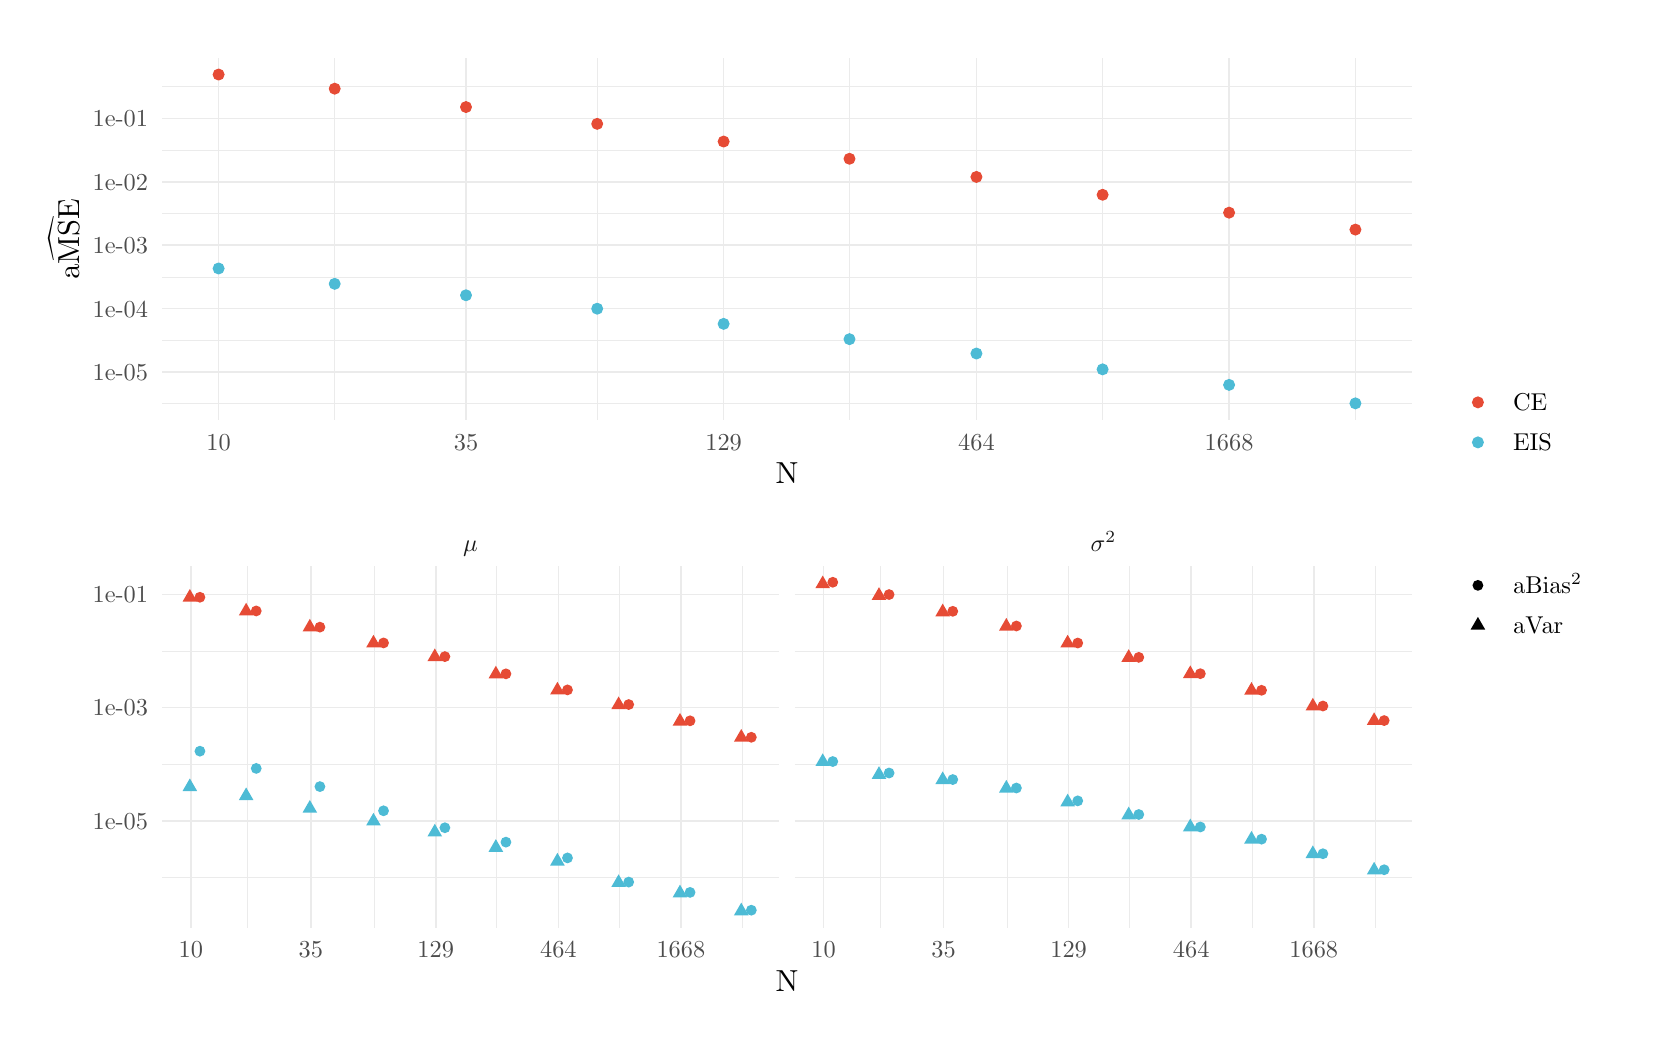
\begin{tikzpicture}[x=1pt,y=1pt]
\definecolor{fillColor}{RGB}{255,255,255}
\path[use as bounding box,fill=fillColor,fill opacity=0.00] (0,0) rectangle (578.16,361.35);
\begin{scope}
\path[clip] ( 48.45,219.65) rectangle (500.31,350.35);
\definecolor{drawColor}{gray}{0.92}

\path[draw=drawColor,line width= 0.3pt,line join=round] ( 48.45,225.46) --
	(500.31,225.46);

\path[draw=drawColor,line width= 0.3pt,line join=round] ( 48.45,248.36) --
	(500.31,248.36);

\path[draw=drawColor,line width= 0.3pt,line join=round] ( 48.45,271.25) --
	(500.31,271.25);

\path[draw=drawColor,line width= 0.3pt,line join=round] ( 48.45,294.15) --
	(500.31,294.15);

\path[draw=drawColor,line width= 0.3pt,line join=round] ( 48.45,317.04) --
	(500.31,317.04);

\path[draw=drawColor,line width= 0.3pt,line join=round] ( 48.45,339.94) --
	(500.31,339.94);

\path[draw=drawColor,line width= 0.3pt,line join=round] (110.94,219.65) --
	(110.94,350.35);

\path[draw=drawColor,line width= 0.3pt,line join=round] (205.79,219.65) --
	(205.79,350.35);

\path[draw=drawColor,line width= 0.3pt,line join=round] (296.96,219.65) --
	(296.96,350.35);

\path[draw=drawColor,line width= 0.3pt,line join=round] (388.42,219.65) --
	(388.42,350.35);

\path[draw=drawColor,line width= 0.3pt,line join=round] (479.78,219.65) --
	(479.78,350.35);

\path[draw=drawColor,line width= 0.6pt,line join=round] ( 48.45,236.91) --
	(500.31,236.91);

\path[draw=drawColor,line width= 0.6pt,line join=round] ( 48.45,259.81) --
	(500.31,259.81);

\path[draw=drawColor,line width= 0.6pt,line join=round] ( 48.45,282.70) --
	(500.31,282.70);

\path[draw=drawColor,line width= 0.6pt,line join=round] ( 48.45,305.60) --
	(500.31,305.60);

\path[draw=drawColor,line width= 0.6pt,line join=round] ( 48.45,328.49) --
	(500.31,328.49);

\path[draw=drawColor,line width= 0.6pt,line join=round] ( 68.99,219.65) --
	( 68.99,350.35);

\path[draw=drawColor,line width= 0.6pt,line join=round] (158.39,219.65) --
	(158.39,350.35);

\path[draw=drawColor,line width= 0.6pt,line join=round] (251.48,219.65) --
	(251.48,350.35);

\path[draw=drawColor,line width= 0.6pt,line join=round] (342.83,219.65) --
	(342.83,350.35);

\path[draw=drawColor,line width= 0.6pt,line join=round] (434.13,219.65) --
	(434.13,350.35);
\definecolor{drawColor}{RGB}{230,75,53}
\definecolor{fillColor}{RGB}{230,75,53}

\path[draw=drawColor,line width= 0.4pt,line join=round,line cap=round,fill=fillColor] ( 68.99,344.41) circle (  1.96);

\path[draw=drawColor,line width= 0.4pt,line join=round,line cap=round,fill=fillColor] (110.94,339.30) circle (  1.96);

\path[draw=drawColor,line width= 0.4pt,line join=round,line cap=round,fill=fillColor] (158.39,332.66) circle (  1.96);

\path[draw=drawColor,line width= 0.4pt,line join=round,line cap=round,fill=fillColor] (205.79,326.59) circle (  1.96);

\path[draw=drawColor,line width= 0.4pt,line join=round,line cap=round,fill=fillColor] (251.48,320.20) circle (  1.96);

\path[draw=drawColor,line width= 0.4pt,line join=round,line cap=round,fill=fillColor] (296.96,313.97) circle (  1.96);

\path[draw=drawColor,line width= 0.4pt,line join=round,line cap=round,fill=fillColor] (342.83,307.41) circle (  1.96);

\path[draw=drawColor,line width= 0.4pt,line join=round,line cap=round,fill=fillColor] (388.42,300.96) circle (  1.96);

\path[draw=drawColor,line width= 0.4pt,line join=round,line cap=round,fill=fillColor] (434.13,294.50) circle (  1.96);

\path[draw=drawColor,line width= 0.4pt,line join=round,line cap=round,fill=fillColor] (479.78,288.38) circle (  1.96);
\definecolor{drawColor}{RGB}{77,187,213}
\definecolor{fillColor}{RGB}{77,187,213}

\path[draw=drawColor,line width= 0.4pt,line join=round,line cap=round,fill=fillColor] ( 68.99,274.33) circle (  1.96);

\path[draw=drawColor,line width= 0.4pt,line join=round,line cap=round,fill=fillColor] (110.94,268.78) circle (  1.96);

\path[draw=drawColor,line width= 0.4pt,line join=round,line cap=round,fill=fillColor] (158.39,264.65) circle (  1.96);

\path[draw=drawColor,line width= 0.4pt,line join=round,line cap=round,fill=fillColor] (205.79,259.80) circle (  1.96);

\path[draw=drawColor,line width= 0.4pt,line join=round,line cap=round,fill=fillColor] (251.48,254.32) circle (  1.96);

\path[draw=drawColor,line width= 0.4pt,line join=round,line cap=round,fill=fillColor] (296.96,248.79) circle (  1.96);

\path[draw=drawColor,line width= 0.4pt,line join=round,line cap=round,fill=fillColor] (342.83,243.60) circle (  1.96);

\path[draw=drawColor,line width= 0.4pt,line join=round,line cap=round,fill=fillColor] (388.42,237.88) circle (  1.96);

\path[draw=drawColor,line width= 0.4pt,line join=round,line cap=round,fill=fillColor] (434.13,232.27) circle (  1.96);

\path[draw=drawColor,line width= 0.4pt,line join=round,line cap=round,fill=fillColor] (479.78,225.59) circle (  1.96);
\end{scope}
\begin{scope}
\path[clip] (  0.00,  0.00) rectangle (578.16,361.35);
\definecolor{drawColor}{gray}{0.30}

\node[text=drawColor,anchor=base east,inner sep=0pt, outer sep=0pt, scale=  0.88] at ( 43.50,233.88) {1e-05};

\node[text=drawColor,anchor=base east,inner sep=0pt, outer sep=0pt, scale=  0.88] at ( 43.50,256.78) {1e-04};

\node[text=drawColor,anchor=base east,inner sep=0pt, outer sep=0pt, scale=  0.88] at ( 43.50,279.67) {1e-03};

\node[text=drawColor,anchor=base east,inner sep=0pt, outer sep=0pt, scale=  0.88] at ( 43.50,302.57) {1e-02};

\node[text=drawColor,anchor=base east,inner sep=0pt, outer sep=0pt, scale=  0.88] at ( 43.50,325.46) {1e-01};
\end{scope}
\begin{scope}
\path[clip] (  0.00,  0.00) rectangle (578.16,361.35);
\definecolor{drawColor}{gray}{0.30}

\node[text=drawColor,anchor=base,inner sep=0pt, outer sep=0pt, scale=  0.88] at ( 68.99,208.64) {10};

\node[text=drawColor,anchor=base,inner sep=0pt, outer sep=0pt, scale=  0.88] at (158.39,208.64) {35};

\node[text=drawColor,anchor=base,inner sep=0pt, outer sep=0pt, scale=  0.88] at (251.48,208.64) {129};

\node[text=drawColor,anchor=base,inner sep=0pt, outer sep=0pt, scale=  0.88] at (342.83,208.64) {464};

\node[text=drawColor,anchor=base,inner sep=0pt, outer sep=0pt, scale=  0.88] at (434.13,208.64) {1668};
\end{scope}
\begin{scope}
\path[clip] (  0.00,  0.00) rectangle (578.16,361.35);
\definecolor{drawColor}{RGB}{0,0,0}

\node[text=drawColor,anchor=base,inner sep=0pt, outer sep=0pt, scale=  1.10] at (274.38,196.60) {N};
\end{scope}
\begin{scope}
\path[clip] (  0.00,  0.00) rectangle (578.16,361.35);
\definecolor{drawColor}{RGB}{0,0,0}

\node[text=drawColor,rotate= 90.00,anchor=base,inner sep=0pt, outer sep=0pt, scale=  1.10] at ( 18.58,285.00) {$\widehat{\mathrm{aMSE}}$};
\end{scope}
\begin{scope}
\path[clip] ( 48.45, 36.19) rectangle (271.63,166.89);
\definecolor{drawColor}{gray}{0.92}

\path[draw=drawColor,line width= 0.3pt,line join=round] ( 48.45, 54.35) --
	(271.63, 54.35);

\path[draw=drawColor,line width= 0.3pt,line join=round] ( 48.45, 95.22) --
	(271.63, 95.22);

\path[draw=drawColor,line width= 0.3pt,line join=round] ( 48.45,136.10) --
	(271.63,136.10);

\path[draw=drawColor,line width= 0.3pt,line join=round] ( 79.29, 36.19) --
	( 79.29,166.89);

\path[draw=drawColor,line width= 0.3pt,line join=round] (125.29, 36.19) --
	(125.29,166.89);

\path[draw=drawColor,line width= 0.3pt,line join=round] (169.52, 36.19) --
	(169.52,166.89);

\path[draw=drawColor,line width= 0.3pt,line join=round] (213.88, 36.19) --
	(213.88,166.89);

\path[draw=drawColor,line width= 0.3pt,line join=round] (258.19, 36.19) --
	(258.19,166.89);

\path[draw=drawColor,line width= 0.6pt,line join=round] ( 48.45, 74.78) --
	(271.63, 74.78);

\path[draw=drawColor,line width= 0.6pt,line join=round] ( 48.45,115.66) --
	(271.63,115.66);

\path[draw=drawColor,line width= 0.6pt,line join=round] ( 48.45,156.54) --
	(271.63,156.54);

\path[draw=drawColor,line width= 0.6pt,line join=round] ( 58.94, 36.19) --
	( 58.94,166.89);

\path[draw=drawColor,line width= 0.6pt,line join=round] (102.31, 36.19) --
	(102.31,166.89);

\path[draw=drawColor,line width= 0.6pt,line join=round] (147.46, 36.19) --
	(147.46,166.89);

\path[draw=drawColor,line width= 0.6pt,line join=round] (191.76, 36.19) --
	(191.76,166.89);

\path[draw=drawColor,line width= 0.6pt,line join=round] (236.05, 36.19) --
	(236.05,166.89);
\definecolor{fillColor}{RGB}{230,75,53}

\path[fill=fillColor] ( 62.24,155.53) circle (  1.96);

\path[fill=fillColor] ( 58.60,158.52) --
	( 61.24,153.94) --
	( 55.96,153.94) --
	cycle;
\definecolor{fillColor}{RGB}{77,187,213}

\path[fill=fillColor] ( 62.24, 99.91) circle (  1.96);

\path[fill=fillColor] ( 58.60, 90.07) --
	( 61.24, 85.50) --
	( 55.96, 85.50) --
	cycle;
\definecolor{fillColor}{RGB}{230,75,53}

\path[fill=fillColor] ( 82.59,150.58) circle (  1.96);

\path[fill=fillColor] ( 78.94,153.54) --
	( 81.59,148.96) --
	( 76.30,148.96) --
	cycle;
\definecolor{fillColor}{RGB}{77,187,213}

\path[fill=fillColor] ( 82.59, 93.68) circle (  1.96);

\path[fill=fillColor] ( 78.94, 86.81) --
	( 81.59, 82.23) --
	( 76.30, 82.23) --
	cycle;
\definecolor{fillColor}{RGB}{230,75,53}

\path[fill=fillColor] (105.60,144.73) circle (  1.96);

\path[fill=fillColor] (101.96,147.73) --
	(104.60,143.16) --
	( 99.32,143.16) --
	cycle;
\definecolor{fillColor}{RGB}{77,187,213}

\path[fill=fillColor] (105.60, 87.11) circle (  1.96);

\path[fill=fillColor] (101.96, 82.27) --
	(104.60, 77.69) --
	( 99.32, 77.69) --
	cycle;
\definecolor{fillColor}{RGB}{230,75,53}

\path[fill=fillColor] (128.59,139.02) circle (  1.96);

\path[fill=fillColor] (124.95,141.97) --
	(127.59,137.39) --
	(122.31,137.39) --
	cycle;
\definecolor{fillColor}{RGB}{77,187,213}

\path[fill=fillColor] (128.59, 78.37) circle (  1.96);

\path[fill=fillColor] (124.95, 77.65) --
	(127.59, 73.08) --
	(122.31, 73.08) --
	cycle;
\definecolor{fillColor}{RGB}{230,75,53}

\path[fill=fillColor] (150.76,134.08) circle (  1.96);

\path[fill=fillColor] (147.11,137.03) --
	(149.76,132.45) --
	(144.47,132.45) --
	cycle;
\definecolor{fillColor}{RGB}{77,187,213}

\path[fill=fillColor] (150.76, 72.24) circle (  1.96);

\path[fill=fillColor] (147.11, 73.68) --
	(149.76, 69.11) --
	(144.47, 69.11) --
	cycle;
\definecolor{fillColor}{RGB}{230,75,53}

\path[fill=fillColor] (172.82,127.85) circle (  1.96);

\path[fill=fillColor] (169.17,130.78) --
	(171.82,126.20) --
	(166.53,126.20) --
	cycle;
\definecolor{fillColor}{RGB}{77,187,213}

\path[fill=fillColor] (172.82, 67.04) circle (  1.96);

\path[fill=fillColor] (169.17, 68.14) --
	(171.82, 63.56) --
	(166.53, 63.56) --
	cycle;
\definecolor{fillColor}{RGB}{230,75,53}

\path[fill=fillColor] (195.06,122.05) circle (  1.96);

\path[fill=fillColor] (191.42,124.98) --
	(194.06,120.40) --
	(188.78,120.40) --
	cycle;
\definecolor{fillColor}{RGB}{77,187,213}

\path[fill=fillColor] (195.06, 61.34) circle (  1.96);

\path[fill=fillColor] (191.42, 63.18) --
	(194.06, 58.60) --
	(188.78, 58.60) --
	cycle;
\definecolor{fillColor}{RGB}{230,75,53}

\path[fill=fillColor] (217.18,116.76) circle (  1.96);

\path[fill=fillColor] (213.53,119.68) --
	(216.18,115.11) --
	(210.89,115.11) --
	cycle;
\definecolor{fillColor}{RGB}{77,187,213}

\path[fill=fillColor] (217.18, 52.61) circle (  1.96);

\path[fill=fillColor] (213.53, 55.43) --
	(216.18, 50.85) --
	(210.89, 50.85) --
	cycle;
\definecolor{fillColor}{RGB}{230,75,53}

\path[fill=fillColor] (239.35,110.88) circle (  1.96);

\path[fill=fillColor] (235.71,113.73) --
	(238.35,109.15) --
	(233.07,109.15) --
	cycle;
\definecolor{fillColor}{RGB}{77,187,213}

\path[fill=fillColor] (239.35, 48.88) circle (  1.96);

\path[fill=fillColor] (235.71, 51.68) --
	(238.35, 47.10) --
	(233.07, 47.10) --
	cycle;
\definecolor{fillColor}{RGB}{230,75,53}

\path[fill=fillColor] (261.49,104.93) circle (  1.96);

\path[fill=fillColor] (257.85,107.91) --
	(260.49,103.33) --
	(255.20,103.33) --
	cycle;
\definecolor{fillColor}{RGB}{77,187,213}

\path[fill=fillColor] (261.49, 42.45) circle (  1.96);

\path[fill=fillColor] (257.85, 45.18) --
	(260.49, 40.60) --
	(255.20, 40.60) --
	cycle;
\end{scope}
\begin{scope}
\path[clip] (277.13, 36.19) rectangle (500.31,166.89);
\definecolor{drawColor}{gray}{0.92}

\path[draw=drawColor,line width= 0.3pt,line join=round] (277.13, 54.35) --
	(500.31, 54.35);

\path[draw=drawColor,line width= 0.3pt,line join=round] (277.13, 95.22) --
	(500.31, 95.22);

\path[draw=drawColor,line width= 0.3pt,line join=round] (277.13,136.10) --
	(500.31,136.10);

\path[draw=drawColor,line width= 0.3pt,line join=round] (307.97, 36.19) --
	(307.97,166.89);

\path[draw=drawColor,line width= 0.3pt,line join=round] (353.97, 36.19) --
	(353.97,166.89);

\path[draw=drawColor,line width= 0.3pt,line join=round] (398.20, 36.19) --
	(398.20,166.89);

\path[draw=drawColor,line width= 0.3pt,line join=round] (442.56, 36.19) --
	(442.56,166.89);

\path[draw=drawColor,line width= 0.3pt,line join=round] (486.87, 36.19) --
	(486.87,166.89);

\path[draw=drawColor,line width= 0.6pt,line join=round] (277.13, 74.78) --
	(500.31, 74.78);

\path[draw=drawColor,line width= 0.6pt,line join=round] (277.13,115.66) --
	(500.31,115.66);

\path[draw=drawColor,line width= 0.6pt,line join=round] (277.13,156.54) --
	(500.31,156.54);

\path[draw=drawColor,line width= 0.6pt,line join=round] (287.62, 36.19) --
	(287.62,166.89);

\path[draw=drawColor,line width= 0.6pt,line join=round] (330.99, 36.19) --
	(330.99,166.89);

\path[draw=drawColor,line width= 0.6pt,line join=round] (376.14, 36.19) --
	(376.14,166.89);

\path[draw=drawColor,line width= 0.6pt,line join=round] (420.45, 36.19) --
	(420.45,166.89);

\path[draw=drawColor,line width= 0.6pt,line join=round] (464.73, 36.19) --
	(464.73,166.89);
\definecolor{fillColor}{RGB}{230,75,53}

\path[fill=fillColor] (290.92,160.95) circle (  1.96);

\path[fill=fillColor] (287.28,163.39) --
	(289.92,158.82) --
	(284.64,158.82) --
	cycle;
\definecolor{fillColor}{RGB}{77,187,213}

\path[fill=fillColor] (290.92, 96.17) circle (  1.96);

\path[fill=fillColor] (287.28, 99.14) --
	(289.92, 94.56) --
	(284.64, 94.56) --
	cycle;
\definecolor{fillColor}{RGB}{230,75,53}

\path[fill=fillColor] (311.27,156.50) circle (  1.96);

\path[fill=fillColor] (307.62,159.16) --
	(310.27,154.59) --
	(304.98,154.59) --
	cycle;
\definecolor{fillColor}{RGB}{77,187,213}

\path[fill=fillColor] (311.27, 92.02) circle (  1.96);

\path[fill=fillColor] (307.62, 94.48) --
	(310.27, 89.90) --
	(304.98, 89.90) --
	cycle;
\definecolor{fillColor}{RGB}{230,75,53}

\path[fill=fillColor] (334.28,150.45) circle (  1.96);

\path[fill=fillColor] (330.64,153.24) --
	(333.28,148.66) --
	(328.00,148.66) --
	cycle;
\definecolor{fillColor}{RGB}{77,187,213}

\path[fill=fillColor] (334.28, 89.66) circle (  1.96);

\path[fill=fillColor] (330.64, 92.60) --
	(333.28, 88.03) --
	(328.00, 88.03) --
	cycle;
\definecolor{fillColor}{RGB}{230,75,53}

\path[fill=fillColor] (357.27,145.14) circle (  1.96);

\path[fill=fillColor] (353.63,148.06) --
	(356.27,143.48) --
	(350.99,143.48) --
	cycle;
\definecolor{fillColor}{RGB}{77,187,213}

\path[fill=fillColor] (357.27, 86.60) circle (  1.96);

\path[fill=fillColor] (353.63, 89.53) --
	(356.27, 84.96) --
	(350.99, 84.96) --
	cycle;
\definecolor{fillColor}{RGB}{230,75,53}

\path[fill=fillColor] (379.44,138.99) circle (  1.96);

\path[fill=fillColor] (375.79,141.98) --
	(378.44,137.40) --
	(373.15,137.40) --
	cycle;
\definecolor{fillColor}{RGB}{77,187,213}

\path[fill=fillColor] (379.44, 81.96) circle (  1.96);

\path[fill=fillColor] (375.79, 84.57) --
	(378.44, 79.99) --
	(373.15, 79.99) --
	cycle;
\definecolor{fillColor}{RGB}{230,75,53}

\path[fill=fillColor] (401.50,133.81) circle (  1.96);

\path[fill=fillColor] (397.85,136.77) --
	(400.50,132.19) --
	(395.21,132.19) --
	cycle;
\definecolor{fillColor}{RGB}{77,187,213}

\path[fill=fillColor] (401.50, 77.03) circle (  1.96);

\path[fill=fillColor] (397.85, 79.89) --
	(400.50, 75.31) --
	(395.21, 75.31) --
	cycle;
\definecolor{fillColor}{RGB}{230,75,53}

\path[fill=fillColor] (423.74,127.91) circle (  1.96);

\path[fill=fillColor] (420.10,130.90) --
	(422.74,126.32) --
	(417.46,126.32) --
	cycle;
\definecolor{fillColor}{RGB}{77,187,213}

\path[fill=fillColor] (423.74, 72.52) circle (  1.96);

\path[fill=fillColor] (420.10, 75.55) --
	(422.74, 70.97) --
	(417.46, 70.97) --
	cycle;
\definecolor{fillColor}{RGB}{230,75,53}

\path[fill=fillColor] (445.86,121.91) circle (  1.96);

\path[fill=fillColor] (442.22,124.89) --
	(444.86,120.31) --
	(439.57,120.31) --
	cycle;
\definecolor{fillColor}{RGB}{77,187,213}

\path[fill=fillColor] (445.86, 68.12) circle (  1.96);

\path[fill=fillColor] (442.22, 71.10) --
	(444.86, 66.52) --
	(439.57, 66.52) --
	cycle;
\definecolor{fillColor}{RGB}{230,75,53}

\path[fill=fillColor] (468.03,116.23) circle (  1.96);

\path[fill=fillColor] (464.39,119.19) --
	(467.03,114.61) --
	(461.75,114.61) --
	cycle;
\definecolor{fillColor}{RGB}{77,187,213}

\path[fill=fillColor] (468.03, 62.85) circle (  1.96);

\path[fill=fillColor] (464.39, 65.87) --
	(467.03, 61.29) --
	(461.75, 61.29) --
	cycle;
\definecolor{fillColor}{RGB}{230,75,53}

\path[fill=fillColor] (490.17,110.97) circle (  1.96);

\path[fill=fillColor] (486.53,113.96) --
	(489.17,109.39) --
	(483.88,109.39) --
	cycle;
\definecolor{fillColor}{RGB}{77,187,213}

\path[fill=fillColor] (490.17, 57.06) circle (  1.96);

\path[fill=fillColor] (486.53, 59.93) --
	(489.17, 55.35) --
	(483.88, 55.35) --
	cycle;
\end{scope}
\begin{scope}
\path[clip] ( 48.45,166.89) rectangle (271.63,183.46);
\definecolor{drawColor}{gray}{0.10}

\node[text=drawColor,anchor=base,inner sep=0pt, outer sep=0pt, scale=  0.88] at (160.04,172.14) {$\mu$};
\end{scope}
\begin{scope}
\path[clip] (277.13,166.89) rectangle (500.31,183.46);
\definecolor{drawColor}{gray}{0.10}

\node[text=drawColor,anchor=base,inner sep=0pt, outer sep=0pt, scale=  0.88] at (388.72,172.14) {$\sigma^2$};
\end{scope}
\begin{scope}
\path[clip] (  0.00,  0.00) rectangle (578.16,361.35);
\definecolor{drawColor}{gray}{0.30}

\node[text=drawColor,anchor=base,inner sep=0pt, outer sep=0pt, scale=  0.88] at ( 58.94, 25.18) {10};

\node[text=drawColor,anchor=base,inner sep=0pt, outer sep=0pt, scale=  0.88] at (102.31, 25.18) {35};

\node[text=drawColor,anchor=base,inner sep=0pt, outer sep=0pt, scale=  0.88] at (147.46, 25.18) {129};

\node[text=drawColor,anchor=base,inner sep=0pt, outer sep=0pt, scale=  0.88] at (191.76, 25.18) {464};

\node[text=drawColor,anchor=base,inner sep=0pt, outer sep=0pt, scale=  0.88] at (236.05, 25.18) {1668};
\end{scope}
\begin{scope}
\path[clip] (  0.00,  0.00) rectangle (578.16,361.35);
\definecolor{drawColor}{gray}{0.30}

\node[text=drawColor,anchor=base,inner sep=0pt, outer sep=0pt, scale=  0.88] at (287.62, 25.18) {10};

\node[text=drawColor,anchor=base,inner sep=0pt, outer sep=0pt, scale=  0.88] at (330.99, 25.18) {35};

\node[text=drawColor,anchor=base,inner sep=0pt, outer sep=0pt, scale=  0.88] at (376.14, 25.18) {129};

\node[text=drawColor,anchor=base,inner sep=0pt, outer sep=0pt, scale=  0.88] at (420.45, 25.18) {464};

\node[text=drawColor,anchor=base,inner sep=0pt, outer sep=0pt, scale=  0.88] at (464.73, 25.18) {1668};
\end{scope}
\begin{scope}
\path[clip] (  0.00,  0.00) rectangle (578.16,361.35);
\definecolor{drawColor}{gray}{0.30}

\node[text=drawColor,anchor=base east,inner sep=0pt, outer sep=0pt, scale=  0.88] at ( 43.50, 71.75) {1e-05};

\node[text=drawColor,anchor=base east,inner sep=0pt, outer sep=0pt, scale=  0.88] at ( 43.50,112.63) {1e-03};

\node[text=drawColor,anchor=base east,inner sep=0pt, outer sep=0pt, scale=  0.88] at ( 43.50,153.51) {1e-01};
\end{scope}
\begin{scope}
\path[clip] (  0.00,  0.00) rectangle (578.16,361.35);
\definecolor{drawColor}{RGB}{0,0,0}

\node[text=drawColor,anchor=base,inner sep=0pt, outer sep=0pt, scale=  1.10] at (274.38, 13.14) {N};
\end{scope}
\begin{scope}
\path[clip] (  0.00,  0.00) rectangle (578.16,361.35);
\definecolor{drawColor}{RGB}{230,75,53}
\definecolor{fillColor}{RGB}{230,75,53}

\path[draw=drawColor,line width= 0.4pt,line join=round,line cap=round,fill=fillColor] (524.04,225.95) circle (  1.96);
\end{scope}
\begin{scope}
\path[clip] (  0.00,  0.00) rectangle (578.16,361.35);
\definecolor{drawColor}{RGB}{77,187,213}
\definecolor{fillColor}{RGB}{77,187,213}

\path[draw=drawColor,line width= 0.4pt,line join=round,line cap=round,fill=fillColor] (524.04,211.49) circle (  1.96);
\end{scope}
\begin{scope}
\path[clip] (  0.00,  0.00) rectangle (578.16,361.35);
\definecolor{drawColor}{RGB}{0,0,0}

\node[text=drawColor,anchor=base west,inner sep=0pt, outer sep=0pt, scale=  0.88] at (536.77,222.92) {CE};
\end{scope}
\begin{scope}
\path[clip] (  0.00,  0.00) rectangle (578.16,361.35);
\definecolor{drawColor}{RGB}{0,0,0}

\node[text=drawColor,anchor=base west,inner sep=0pt, outer sep=0pt, scale=  0.88] at (536.77,208.46) {EIS};
\end{scope}
\begin{scope}
\path[clip] (  0.00,  0.00) rectangle (578.16,361.35);
\definecolor{fillColor}{RGB}{0,0,0}

\path[fill=fillColor] (524.04,159.83) circle (  1.96);
\end{scope}
\begin{scope}
\path[clip] (  0.00,  0.00) rectangle (578.16,361.35);
\definecolor{fillColor}{RGB}{0,0,0}

\path[fill=fillColor] (524.04,148.42) --
	(526.68,143.85) --
	(521.40,143.85) --
	cycle;
\end{scope}
\begin{scope}
\path[clip] (  0.00,  0.00) rectangle (578.16,361.35);
\definecolor{drawColor}{RGB}{0,0,0}

\node[text=drawColor,anchor=base west,inner sep=0pt, outer sep=0pt, scale=  0.88] at (536.77,156.80) {aBias$^2$};
\end{scope}
\begin{scope}
\path[clip] (  0.00,  0.00) rectangle (578.16,361.35);
\definecolor{drawColor}{RGB}{0,0,0}

\node[text=drawColor,anchor=base west,inner sep=0pt, outer sep=0pt, scale=  0.88] at (536.77,142.34) {aVar};
\end{scope}
\end{tikzpicture}

    }
    \caption{{\color{red} TODO}}
    \label{fig:mse_bias_var_decomposition}
\end{figure}

% fig:mse_bias_var_decomposition
\todo{interpretation of \Cref{fig:mse_bias_var_decomposition}, equal contribution of bias and var, not much to gain from bias correction}


\subsection{Numerical convergence}
\label{subsec:numerical-convergence}

\subsection{Performance of the optimal proposal}
\label{subsec:performance_at_optimal}
\todo{change EF to aEF (asymptotic EF) everywhere in this section}
For the performance of importance sampling the efficiency factor $ \text{EF} = \frac{\text{ESS}}{N}$ plays an important role, see \Cref{sec:importance_sampling}. Additionally, it allows a comparison of the effectiveness of importance sampling across multiple sample sizes $N$, indeed, as $N\to\infty$, $\text{EF}$ converges to $ \rho^{-1}$, where $\rho$ is the second moment of importance sampling weights, $\int w^{2} \d \G$.

Returning to the distributions studied in \Cref{ex:univ-gaussian-s2-fixed,ex:univ-gaussian-mu-fixed}, we now calculate the asymptotic efficiency factor
$$
\text{EF} = \frac{1}{\rho} \in (0, 1].
$$
As the proposal is always $\mathcal N(\mu, \sigma^{2})$ with either $\mu$ or $\sigma^{2}$ fixed, and $\P$ is a mixture of Gaussians or $\mathcal N(0,1)$, $\rho$ is analytically available. 

For \Cref{ex:univ-gaussian-s2-fixed}, both \aeis and the \acem have, by symmetry, the same optimal $\mu = 0$. Thus the efficiency factor only depends on the fixed $\sigma^{2}$, see \Cref{fig:rho_mu}, and is the same for \aeis and the \acem.

\begin{figure}
    \centering
    \resizebox{\textwidth}{!}{%
        % Created by tikzDevice version 0.12.6 on 2024-06-10 16:57:56
% !TEX encoding = UTF-8 Unicode
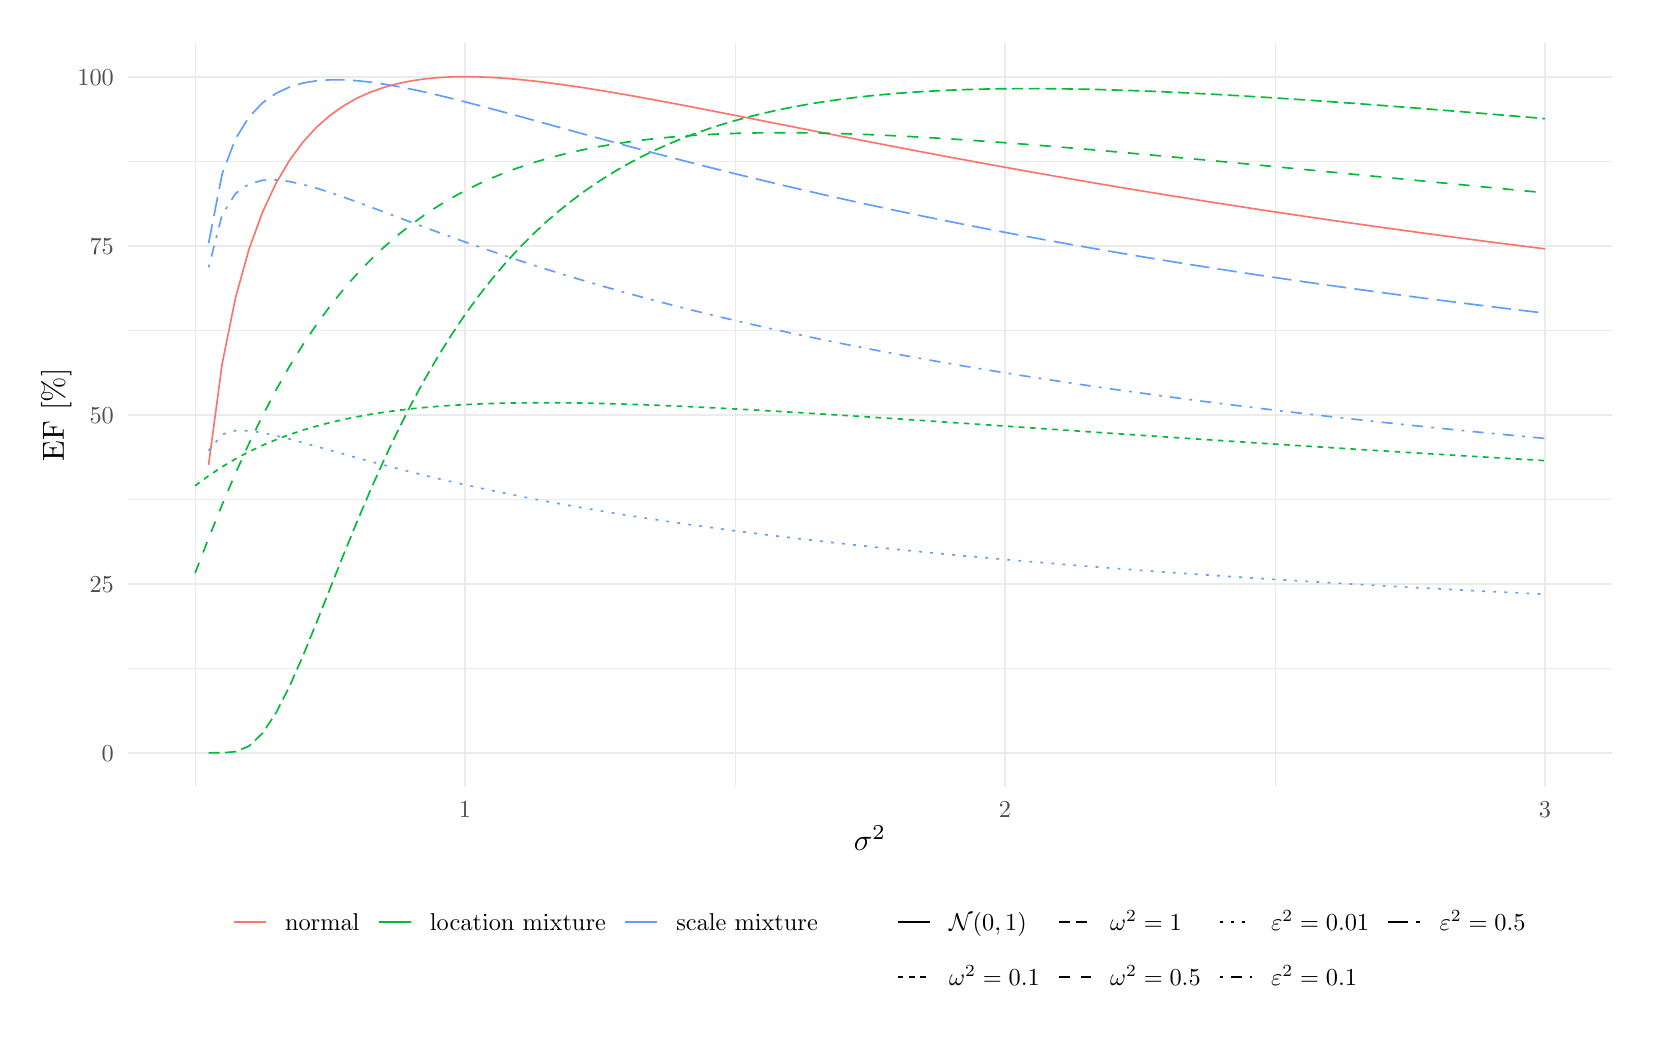
\begin{tikzpicture}[x=1pt,y=1pt]
\definecolor{fillColor}{RGB}{255,255,255}
\path[use as bounding box,fill=fillColor,fill opacity=0.00] (0,0) rectangle (578.16,361.35);
\begin{scope}
\path[clip] ( 36.11, 87.09) rectangle (572.66,355.85);
\definecolor{drawColor}{gray}{0.92}

\path[draw=drawColor,line width= 0.3pt,line join=round] ( 36.11,129.85) --
	(572.66,129.85);

\path[draw=drawColor,line width= 0.3pt,line join=round] ( 36.11,190.93) --
	(572.66,190.93);

\path[draw=drawColor,line width= 0.3pt,line join=round] ( 36.11,252.01) --
	(572.66,252.01);

\path[draw=drawColor,line width= 0.3pt,line join=round] ( 36.11,313.09) --
	(572.66,313.09);

\path[draw=drawColor,line width= 0.3pt,line join=round] ( 60.50, 87.09) --
	( 60.50,355.85);

\path[draw=drawColor,line width= 0.3pt,line join=round] (255.61, 87.09) --
	(255.61,355.85);

\path[draw=drawColor,line width= 0.3pt,line join=round] (450.72, 87.09) --
	(450.72,355.85);

\path[draw=drawColor,line width= 0.6pt,line join=round] ( 36.11, 99.31) --
	(572.66, 99.31);

\path[draw=drawColor,line width= 0.6pt,line join=round] ( 36.11,160.39) --
	(572.66,160.39);

\path[draw=drawColor,line width= 0.6pt,line join=round] ( 36.11,221.47) --
	(572.66,221.47);

\path[draw=drawColor,line width= 0.6pt,line join=round] ( 36.11,282.55) --
	(572.66,282.55);

\path[draw=drawColor,line width= 0.6pt,line join=round] ( 36.11,343.63) --
	(572.66,343.63);

\path[draw=drawColor,line width= 0.6pt,line join=round] (158.05, 87.09) --
	(158.05,355.85);

\path[draw=drawColor,line width= 0.6pt,line join=round] (353.16, 87.09) --
	(353.16,355.85);

\path[draw=drawColor,line width= 0.6pt,line join=round] (548.27, 87.09) --
	(548.27,355.85);
\definecolor{drawColor}{RGB}{248,118,109}

\path[draw=drawColor,line width= 0.6pt,line join=round] ( 65.38,203.37) --
	( 70.26,239.79) --
	( 75.13,263.88) --
	( 80.01,281.42) --
	( 84.89,294.77) --
	( 89.77,305.19) --
	( 94.64,313.45) --
	( 99.52,320.06) --
	(104.40,325.38) --
	(109.28,329.66) --
	(114.15,333.11) --
	(119.03,335.88) --
	(123.91,338.07) --
	(128.79,339.80) --
	(133.67,341.13) --
	(138.54,342.12) --
	(143.42,342.83) --
	(148.30,343.30) --
	(153.18,343.55) --
	(158.05,343.63) --
	(162.93,343.56) --
	(167.81,343.36) --
	(172.69,343.04) --
	(177.56,342.62) --
	(182.44,342.12) --
	(187.32,341.55) --
	(192.20,340.91) --
	(197.08,340.22) --
	(201.95,339.48) --
	(206.83,338.70) --
	(211.71,337.88) --
	(216.59,337.04) --
	(221.46,336.17) --
	(226.34,335.28) --
	(231.22,334.37) --
	(236.10,333.45) --
	(240.98,332.51) --
	(245.85,331.57) --
	(250.73,330.62) --
	(255.61,329.66) --
	(260.49,328.70) --
	(265.36,327.74) --
	(270.24,326.77) --
	(275.12,325.80) --
	(280.00,324.84) --
	(284.87,323.88) --
	(289.75,322.92) --
	(294.63,321.96) --
	(299.51,321.01) --
	(304.39,320.06) --
	(309.26,319.11) --
	(314.14,318.18) --
	(319.02,317.24) --
	(323.90,316.32) --
	(328.77,315.40) --
	(333.65,314.48) --
	(338.53,313.58) --
	(343.41,312.68) --
	(348.29,311.79) --
	(353.16,310.90) --
	(358.04,310.02) --
	(362.92,309.15) --
	(367.80,308.29) --
	(372.67,307.43) --
	(377.55,306.59) --
	(382.43,305.75) --
	(387.31,304.91) --
	(392.18,304.09) --
	(397.06,303.27) --
	(401.94,302.46) --
	(406.82,301.66) --
	(411.70,300.86) --
	(416.57,300.08) --
	(421.45,299.30) --
	(426.33,298.52) --
	(431.21,297.76) --
	(436.08,297.00) --
	(440.96,296.25) --
	(445.84,295.51) --
	(450.72,294.77) --
	(455.59,294.04) --
	(460.47,293.32) --
	(465.35,292.60) --
	(470.23,291.89) --
	(475.11,291.19) --
	(479.98,290.50) --
	(484.86,289.81) --
	(489.74,289.12) --
	(494.62,288.45) --
	(499.49,287.78) --
	(504.37,287.12) --
	(509.25,286.46) --
	(514.13,285.81) --
	(519.01,285.16) --
	(523.88,284.52) --
	(528.76,283.89) --
	(533.64,283.26) --
	(538.52,282.64) --
	(543.39,282.03) --
	(548.27,281.42);
\definecolor{drawColor}{RGB}{0,186,56}

\path[draw=drawColor,line width= 0.6pt,dash pattern=on 2pt off 2pt ,line join=round] ( 60.50,195.82) --
	( 65.38,199.43) --
	( 70.26,202.66) --
	( 75.13,205.55) --
	( 80.01,208.13) --
	( 84.89,210.43) --
	( 89.77,212.49) --
	( 94.64,214.31) --
	( 99.52,215.93) --
	(104.40,217.37) --
	(109.28,218.65) --
	(114.15,219.77) --
	(119.03,220.76) --
	(123.91,221.63) --
	(128.79,222.39) --
	(133.67,223.05) --
	(138.54,223.62) --
	(143.42,224.10) --
	(148.30,224.52) --
	(153.18,224.86) --
	(158.05,225.14) --
	(162.93,225.37) --
	(167.81,225.54) --
	(172.69,225.67) --
	(177.56,225.75) --
	(182.44,225.80) --
	(187.32,225.81) --
	(192.20,225.79) --
	(197.08,225.74) --
	(201.95,225.66) --
	(206.83,225.56) --
	(211.71,225.43) --
	(216.59,225.29) --
	(221.46,225.12) --
	(226.34,224.94) --
	(231.22,224.74) --
	(236.10,224.53) --
	(240.98,224.31) --
	(245.85,224.07) --
	(250.73,223.83) --
	(255.61,223.57) --
	(260.49,223.31) --
	(265.36,223.03) --
	(270.24,222.75) --
	(275.12,222.46) --
	(280.00,222.17) --
	(284.87,221.87) --
	(289.75,221.57) --
	(294.63,221.26) --
	(299.51,220.95) --
	(304.39,220.63) --
	(309.26,220.32) --
	(314.14,220.00) --
	(319.02,219.67) --
	(323.90,219.35) --
	(328.77,219.02) --
	(333.65,218.70) --
	(338.53,218.37) --
	(343.41,218.04) --
	(348.29,217.71) --
	(353.16,217.38) --
	(358.04,217.05) --
	(362.92,216.71) --
	(367.80,216.38) --
	(372.67,216.05) --
	(377.55,215.72) --
	(382.43,215.39) --
	(387.31,215.06) --
	(392.18,214.73) --
	(397.06,214.41) --
	(401.94,214.08) --
	(406.82,213.75) --
	(411.70,213.43) --
	(416.57,213.10) --
	(421.45,212.78) --
	(426.33,212.46) --
	(431.21,212.14) --
	(436.08,211.82) --
	(440.96,211.50) --
	(445.84,211.18) --
	(450.72,210.87) --
	(455.59,210.56) --
	(460.47,210.24) --
	(465.35,209.93) --
	(470.23,209.63) --
	(475.11,209.32) --
	(479.98,209.01) --
	(484.86,208.71) --
	(489.74,208.41) --
	(494.62,208.11) --
	(499.49,207.81) --
	(504.37,207.51) --
	(509.25,207.21) --
	(514.13,206.92) --
	(519.01,206.63) --
	(523.88,206.34) --
	(528.76,206.05) --
	(533.64,205.76) --
	(538.52,205.48) --
	(543.39,205.19) --
	(548.27,204.91);

\path[draw=drawColor,line width= 0.6pt,dash pattern=on 4pt off 2pt ,line join=round] ( 65.38, 99.31) --
	( 70.26, 99.32) --
	( 75.13, 99.73) --
	( 80.01,101.76) --
	( 84.89,106.42) --
	( 89.77,113.81) --
	( 94.64,123.40) --
	( 99.52,134.49) --
	(104.40,146.43) --
	(109.28,158.70) --
	(114.15,170.93) --
	(119.03,182.87) --
	(123.91,194.33) --
	(128.79,205.24) --
	(133.67,215.53) --
	(138.54,225.18) --
	(143.42,234.19) --
	(148.30,242.59) --
	(153.18,250.40) --
	(158.05,257.65) --
	(162.93,264.36) --
	(167.81,270.57) --
	(172.69,276.33) --
	(177.56,281.64) --
	(182.44,286.56) --
	(187.32,291.11) --
	(192.20,295.30) --
	(197.08,299.18) --
	(201.95,302.76) --
	(206.83,306.07) --
	(211.71,309.12) --
	(216.59,311.94) --
	(221.46,314.53) --
	(226.34,316.93) --
	(231.22,319.13) --
	(236.10,321.16) --
	(240.98,323.03) --
	(245.85,324.74) --
	(250.73,326.32) --
	(255.61,327.76) --
	(260.49,329.09) --
	(265.36,330.30) --
	(270.24,331.40) --
	(275.12,332.41) --
	(280.00,333.32) --
	(284.87,334.15) --
	(289.75,334.90) --
	(294.63,335.57) --
	(299.51,336.17) --
	(304.39,336.71) --
	(309.26,337.19) --
	(314.14,337.61) --
	(319.02,337.97) --
	(323.90,338.29) --
	(328.77,338.55) --
	(333.65,338.78) --
	(338.53,338.96) --
	(343.41,339.10) --
	(348.29,339.21) --
	(353.16,339.28) --
	(358.04,339.32) --
	(362.92,339.33) --
	(367.80,339.31) --
	(372.67,339.26) --
	(377.55,339.19) --
	(382.43,339.10) --
	(387.31,338.98) --
	(392.18,338.84) --
	(397.06,338.68) --
	(401.94,338.51) --
	(406.82,338.32) --
	(411.70,338.11) --
	(416.57,337.88) --
	(421.45,337.64) --
	(426.33,337.39) --
	(431.21,337.13) --
	(436.08,336.85) --
	(440.96,336.56) --
	(445.84,336.26) --
	(450.72,335.96) --
	(455.59,335.64) --
	(460.47,335.31) --
	(465.35,334.98) --
	(470.23,334.64) --
	(475.11,334.29) --
	(479.98,333.94) --
	(484.86,333.57) --
	(489.74,333.21) --
	(494.62,332.84) --
	(499.49,332.46) --
	(504.37,332.08) --
	(509.25,331.69) --
	(514.13,331.30) --
	(519.01,330.91) --
	(523.88,330.51) --
	(528.76,330.11) --
	(533.64,329.71) --
	(538.52,329.30) --
	(543.39,328.89) --
	(548.27,328.48);

\path[draw=drawColor,line width= 0.6pt,dash pattern=on 4pt off 4pt ,line join=round] ( 60.50,164.25) --
	( 65.38,176.83) --
	( 70.26,188.93) --
	( 75.13,200.39) --
	( 80.01,211.15) --
	( 84.89,221.17) --
	( 89.77,230.45) --
	( 94.64,239.01) --
	( 99.52,246.89) --
	(104.40,254.12) --
	(109.28,260.75) --
	(114.15,266.83) --
	(119.03,272.38) --
	(123.91,277.45) --
	(128.79,282.09) --
	(133.67,286.32) --
	(138.54,290.17) --
	(143.42,293.69) --
	(148.30,296.89) --
	(153.18,299.81) --
	(158.05,302.46) --
	(162.93,304.87) --
	(167.81,307.06) --
	(172.69,309.05) --
	(177.56,310.84) --
	(182.44,312.46) --
	(187.32,313.93) --
	(192.20,315.25) --
	(197.08,316.43) --
	(201.95,317.49) --
	(206.83,318.43) --
	(211.71,319.26) --
	(216.59,320.00) --
	(221.46,320.65) --
	(226.34,321.21) --
	(231.22,321.70) --
	(236.10,322.11) --
	(240.98,322.46) --
	(245.85,322.74) --
	(250.73,322.97) --
	(255.61,323.15) --
	(260.49,323.27) --
	(265.36,323.35) --
	(270.24,323.39) --
	(275.12,323.39) --
	(280.00,323.35) --
	(284.87,323.27) --
	(289.75,323.17) --
	(294.63,323.04) --
	(299.51,322.88) --
	(304.39,322.69) --
	(309.26,322.48) --
	(314.14,322.25) --
	(319.02,322.00) --
	(323.90,321.72) --
	(328.77,321.44) --
	(333.65,321.13) --
	(338.53,320.81) --
	(343.41,320.48) --
	(348.29,320.13) --
	(353.16,319.77) --
	(358.04,319.40) --
	(362.92,319.02) --
	(367.80,318.63) --
	(372.67,318.24) --
	(377.55,317.83) --
	(382.43,317.42) --
	(387.31,317.00) --
	(392.18,316.57) --
	(397.06,316.14) --
	(401.94,315.70) --
	(406.82,315.26) --
	(411.70,314.81) --
	(416.57,314.36) --
	(421.45,313.90) --
	(426.33,313.45) --
	(431.21,312.99) --
	(436.08,312.52) --
	(440.96,312.06) --
	(445.84,311.59) --
	(450.72,311.12) --
	(455.59,310.65) --
	(460.47,310.18) --
	(465.35,309.71) --
	(470.23,309.24) --
	(475.11,308.76) --
	(479.98,308.29) --
	(484.86,307.81) --
	(489.74,307.34) --
	(494.62,306.86) --
	(499.49,306.39) --
	(504.37,305.92) --
	(509.25,305.44) --
	(514.13,304.97) --
	(519.01,304.50) --
	(523.88,304.02) --
	(528.76,303.55) --
	(533.64,303.08) --
	(538.52,302.61) --
	(543.39,302.15) --
	(548.27,301.68);
\definecolor{drawColor}{RGB}{97,156,255}

\path[draw=drawColor,line width= 0.6pt,dash pattern=on 1pt off 3pt ,line join=round] ( 65.38,208.48) --
	( 70.26,214.33) --
	( 75.13,215.76) --
	( 80.01,215.71) --
	( 84.89,214.99) --
	( 89.77,213.93) --
	( 94.64,212.70) --
	( 99.52,211.37) --
	(104.40,210.01) --
	(109.28,208.63) --
	(114.15,207.26) --
	(119.03,205.90) --
	(123.91,204.58) --
	(128.79,203.28) --
	(133.67,202.01) --
	(138.54,200.78) --
	(143.42,199.58) --
	(148.30,198.41) --
	(153.18,197.28) --
	(158.05,196.18) --
	(162.93,195.11) --
	(167.81,194.07) --
	(172.69,193.07) --
	(177.56,192.09) --
	(182.44,191.13) --
	(187.32,190.21) --
	(192.20,189.31) --
	(197.08,188.44) --
	(201.95,187.58) --
	(206.83,186.76) --
	(211.71,185.95) --
	(216.59,185.16) --
	(221.46,184.40) --
	(226.34,183.65) --
	(231.22,182.92) --
	(236.10,182.21) --
	(240.98,181.52) --
	(245.85,180.85) --
	(250.73,180.19) --
	(255.61,179.54) --
	(260.49,178.91) --
	(265.36,178.30) --
	(270.24,177.70) --
	(275.12,177.11) --
	(280.00,176.53) --
	(284.87,175.97) --
	(289.75,175.42) --
	(294.63,174.88) --
	(299.51,174.35) --
	(304.39,173.83) --
	(309.26,173.32) --
	(314.14,172.83) --
	(319.02,172.34) --
	(323.90,171.86) --
	(328.77,171.39) --
	(333.65,170.93) --
	(338.53,170.48) --
	(343.41,170.04) --
	(348.29,169.60) --
	(353.16,169.17) --
	(358.04,168.75) --
	(362.92,168.34) --
	(367.80,167.94) --
	(372.67,167.54) --
	(377.55,167.15) --
	(382.43,166.76) --
	(387.31,166.38) --
	(392.18,166.01) --
	(397.06,165.65) --
	(401.94,165.29) --
	(406.82,164.93) --
	(411.70,164.58) --
	(416.57,164.24) --
	(421.45,163.90) --
	(426.33,163.57) --
	(431.21,163.24) --
	(436.08,162.92) --
	(440.96,162.60) --
	(445.84,162.29) --
	(450.72,161.98) --
	(455.59,161.68) --
	(460.47,161.38) --
	(465.35,161.08) --
	(470.23,160.79) --
	(475.11,160.50) --
	(479.98,160.22) --
	(484.86,159.94) --
	(489.74,159.66) --
	(494.62,159.39) --
	(499.49,159.12) --
	(504.37,158.86) --
	(509.25,158.60) --
	(514.13,158.34) --
	(519.01,158.08) --
	(523.88,157.83) --
	(528.76,157.58) --
	(533.64,157.34) --
	(538.52,157.10) --
	(543.39,156.86) --
	(548.27,156.62);

\path[draw=drawColor,line width= 0.6pt,dash pattern=on 1pt off 3pt on 4pt off 3pt ,line join=round] ( 65.38,274.74) --
	( 70.26,293.74) --
	( 75.13,301.44) --
	( 80.01,304.87) --
	( 84.89,306.20) --
	( 89.77,306.33) --
	( 94.64,305.74) --
	( 99.52,304.68) --
	(104.40,303.33) --
	(109.28,301.78) --
	(114.15,300.11) --
	(119.03,298.35) --
	(123.91,296.55) --
	(128.79,294.72) --
	(133.67,292.88) --
	(138.54,291.05) --
	(143.42,289.23) --
	(148.30,287.43) --
	(153.18,285.66) --
	(158.05,283.91) --
	(162.93,282.19) --
	(167.81,280.51) --
	(172.69,278.86) --
	(177.56,277.24) --
	(182.44,275.65) --
	(187.32,274.10) --
	(192.20,272.58) --
	(197.08,271.09) --
	(201.95,269.63) --
	(206.83,268.21) --
	(211.71,266.82) --
	(216.59,265.45) --
	(221.46,264.12) --
	(226.34,262.81) --
	(231.22,261.54) --
	(236.10,260.28) --
	(240.98,259.06) --
	(245.85,257.86) --
	(250.73,256.68) --
	(255.61,255.53) --
	(260.49,254.41) --
	(265.36,253.30) --
	(270.24,252.22) --
	(275.12,251.16) --
	(280.00,250.12) --
	(284.87,249.09) --
	(289.75,248.09) --
	(294.63,247.11) --
	(299.51,246.15) --
	(304.39,245.20) --
	(309.26,244.27) --
	(314.14,243.36) --
	(319.02,242.46) --
	(323.90,241.58) --
	(328.77,240.72) --
	(333.65,239.87) --
	(338.53,239.04) --
	(343.41,238.22) --
	(348.29,237.41) --
	(353.16,236.62) --
	(358.04,235.84) --
	(362.92,235.07) --
	(367.80,234.32) --
	(372.67,233.58) --
	(377.55,232.85) --
	(382.43,232.13) --
	(387.31,231.42) --
	(392.18,230.72) --
	(397.06,230.04) --
	(401.94,229.36) --
	(406.82,228.70) --
	(411.70,228.04) --
	(416.57,227.40) --
	(421.45,226.76) --
	(426.33,226.13) --
	(431.21,225.51) --
	(436.08,224.91) --
	(440.96,224.31) --
	(445.84,223.71) --
	(450.72,223.13) --
	(455.59,222.55) --
	(460.47,221.99) --
	(465.35,221.43) --
	(470.23,220.87) --
	(475.11,220.33) --
	(479.98,219.79) --
	(484.86,219.26) --
	(489.74,218.73) --
	(494.62,218.22) --
	(499.49,217.71) --
	(504.37,217.20) --
	(509.25,216.70) --
	(514.13,216.21) --
	(519.01,215.72) --
	(523.88,215.24) --
	(528.76,214.77) --
	(533.64,214.30) --
	(538.52,213.84) --
	(543.39,213.38) --
	(548.27,212.93);

\path[draw=drawColor,line width= 0.6pt,dash pattern=on 7pt off 3pt ,line join=round] ( 65.38,283.45) --
	( 70.26,308.45) --
	( 75.13,321.26) --
	( 80.01,329.09) --
	( 84.89,334.21) --
	( 89.77,337.63) --
	( 94.64,339.90) --
	( 99.52,341.33) --
	(104.40,342.15) --
	(109.28,342.50) --
	(114.15,342.48) --
	(119.03,342.18) --
	(123.91,341.66) --
	(128.79,340.95) --
	(133.67,340.11) --
	(138.54,339.14) --
	(143.42,338.09) --
	(148.30,336.96) --
	(153.18,335.77) --
	(158.05,334.54) --
	(162.93,333.27) --
	(167.81,331.97) --
	(172.69,330.66) --
	(177.56,329.33) --
	(182.44,327.99) --
	(187.32,326.65) --
	(192.20,325.30) --
	(197.08,323.96) --
	(201.95,322.62) --
	(206.83,321.29) --
	(211.71,319.97) --
	(216.59,318.65) --
	(221.46,317.35) --
	(226.34,316.05) --
	(231.22,314.77) --
	(236.10,313.51) --
	(240.98,312.25) --
	(245.85,311.01) --
	(250.73,309.79) --
	(255.61,308.58) --
	(260.49,307.38) --
	(265.36,306.20) --
	(270.24,305.03) --
	(275.12,303.88) --
	(280.00,302.74) --
	(284.87,301.62) --
	(289.75,300.51) --
	(294.63,299.42) --
	(299.51,298.34) --
	(304.39,297.28) --
	(309.26,296.23) --
	(314.14,295.19) --
	(319.02,294.17) --
	(323.90,293.16) --
	(328.77,292.16) --
	(333.65,291.18) --
	(338.53,290.21) --
	(343.41,289.26) --
	(348.29,288.31) --
	(353.16,287.38) --
	(358.04,286.46) --
	(362.92,285.56) --
	(367.80,284.66) --
	(372.67,283.78) --
	(377.55,282.91) --
	(382.43,282.04) --
	(387.31,281.19) --
	(392.18,280.36) --
	(397.06,279.53) --
	(401.94,278.71) --
	(406.82,277.90) --
	(411.70,277.10) --
	(416.57,276.31) --
	(421.45,275.54) --
	(426.33,274.77) --
	(431.21,274.01) --
	(436.08,273.26) --
	(440.96,272.52) --
	(445.84,271.79) --
	(450.72,271.06) --
	(455.59,270.35) --
	(460.47,269.64) --
	(465.35,268.94) --
	(470.23,268.25) --
	(475.11,267.57) --
	(479.98,266.89) --
	(484.86,266.23) --
	(489.74,265.57) --
	(494.62,264.92) --
	(499.49,264.27) --
	(504.37,263.63) --
	(509.25,263.00) --
	(514.13,262.38) --
	(519.01,261.76) --
	(523.88,261.15) --
	(528.76,260.55) --
	(533.64,259.95) --
	(538.52,259.36) --
	(543.39,258.78) --
	(548.27,258.20);
\end{scope}
\begin{scope}
\path[clip] (  0.00,  0.00) rectangle (578.16,361.35);
\definecolor{drawColor}{gray}{0.30}

\node[text=drawColor,anchor=base east,inner sep=0pt, outer sep=0pt, scale=  0.88] at ( 31.16, 96.28) {0};

\node[text=drawColor,anchor=base east,inner sep=0pt, outer sep=0pt, scale=  0.88] at ( 31.16,157.36) {25};

\node[text=drawColor,anchor=base east,inner sep=0pt, outer sep=0pt, scale=  0.88] at ( 31.16,218.44) {50};

\node[text=drawColor,anchor=base east,inner sep=0pt, outer sep=0pt, scale=  0.88] at ( 31.16,279.52) {75};

\node[text=drawColor,anchor=base east,inner sep=0pt, outer sep=0pt, scale=  0.88] at ( 31.16,340.60) {100};
\end{scope}
\begin{scope}
\path[clip] (  0.00,  0.00) rectangle (578.16,361.35);
\definecolor{drawColor}{gray}{0.30}

\node[text=drawColor,anchor=base,inner sep=0pt, outer sep=0pt, scale=  0.88] at (158.05, 76.08) {1};

\node[text=drawColor,anchor=base,inner sep=0pt, outer sep=0pt, scale=  0.88] at (353.16, 76.08) {2};

\node[text=drawColor,anchor=base,inner sep=0pt, outer sep=0pt, scale=  0.88] at (548.27, 76.08) {3};
\end{scope}
\begin{scope}
\path[clip] (  0.00,  0.00) rectangle (578.16,361.35);
\definecolor{drawColor}{RGB}{0,0,0}

\node[text=drawColor,anchor=base,inner sep=0pt, outer sep=0pt, scale=  1.10] at (304.39, 64.05) {$\sigma^2$};
\end{scope}
\begin{scope}
\path[clip] (  0.00,  0.00) rectangle (578.16,361.35);
\definecolor{drawColor}{RGB}{0,0,0}

\node[text=drawColor,rotate= 90.00,anchor=base,inner sep=0pt, outer sep=0pt, scale=  1.10] at ( 13.08,221.47) {EF [\%]};
\end{scope}
\begin{scope}
\path[clip] (  0.00,  0.00) rectangle (578.16,361.35);
\definecolor{drawColor}{RGB}{248,118,109}

\path[draw=drawColor,line width= 0.6pt,line join=round] ( 74.48, 38.18) -- ( 86.05, 38.18);
\end{scope}
\begin{scope}
\path[clip] (  0.00,  0.00) rectangle (578.16,361.35);
\definecolor{drawColor}{RGB}{0,186,56}

\path[draw=drawColor,line width= 0.6pt,line join=round] (126.84, 38.18) -- (138.41, 38.18);
\end{scope}
\begin{scope}
\path[clip] (  0.00,  0.00) rectangle (578.16,361.35);
\definecolor{drawColor}{RGB}{97,156,255}

\path[draw=drawColor,line width= 0.6pt,line join=round] (215.86, 38.18) -- (227.43, 38.18);
\end{scope}
\begin{scope}
\path[clip] (  0.00,  0.00) rectangle (578.16,361.35);
\definecolor{drawColor}{RGB}{0,0,0}

\node[text=drawColor,anchor=base west,inner sep=0pt, outer sep=0pt, scale=  0.88] at ( 92.99, 35.15) {normal};
\end{scope}
\begin{scope}
\path[clip] (  0.00,  0.00) rectangle (578.16,361.35);
\definecolor{drawColor}{RGB}{0,0,0}

\node[text=drawColor,anchor=base west,inner sep=0pt, outer sep=0pt, scale=  0.88] at (145.35, 35.15) {location mixture};
\end{scope}
\begin{scope}
\path[clip] (  0.00,  0.00) rectangle (578.16,361.35);
\definecolor{drawColor}{RGB}{0,0,0}

\node[text=drawColor,anchor=base west,inner sep=0pt, outer sep=0pt, scale=  0.88] at (234.37, 35.15) {scale mixture};
\end{scope}
\begin{scope}
\path[clip] (  0.00,  0.00) rectangle (578.16,361.35);
\definecolor{drawColor}{RGB}{0,0,0}

\path[draw=drawColor,line width= 0.6pt,line join=round] (314.47, 38.18) -- (326.03, 38.18);
\end{scope}
\begin{scope}
\path[clip] (  0.00,  0.00) rectangle (578.16,361.35);
\definecolor{drawColor}{RGB}{0,0,0}

\path[draw=drawColor,line width= 0.6pt,dash pattern=on 2pt off 2pt ,line join=round] (314.47, 18.23) -- (326.03, 18.23);
\end{scope}
\begin{scope}
\path[clip] (  0.00,  0.00) rectangle (578.16,361.35);
\definecolor{drawColor}{RGB}{0,0,0}

\path[draw=drawColor,line width= 0.6pt,dash pattern=on 4pt off 2pt ,line join=round] (372.64, 38.18) -- (384.20, 38.18);
\end{scope}
\begin{scope}
\path[clip] (  0.00,  0.00) rectangle (578.16,361.35);
\definecolor{drawColor}{RGB}{0,0,0}

\path[draw=drawColor,line width= 0.6pt,dash pattern=on 4pt off 4pt ,line join=round] (372.64, 18.23) -- (384.20, 18.23);
\end{scope}
\begin{scope}
\path[clip] (  0.00,  0.00) rectangle (578.16,361.35);
\definecolor{drawColor}{RGB}{0,0,0}

\path[draw=drawColor,line width= 0.6pt,dash pattern=on 1pt off 3pt ,line join=round] (430.81, 38.18) -- (442.38, 38.18);
\end{scope}
\begin{scope}
\path[clip] (  0.00,  0.00) rectangle (578.16,361.35);
\definecolor{drawColor}{RGB}{0,0,0}

\path[draw=drawColor,line width= 0.6pt,dash pattern=on 1pt off 3pt on 4pt off 3pt ,line join=round] (430.81, 18.23) -- (442.38, 18.23);
\end{scope}
\begin{scope}
\path[clip] (  0.00,  0.00) rectangle (578.16,361.35);
\definecolor{drawColor}{RGB}{0,0,0}

\path[draw=drawColor,line width= 0.6pt,dash pattern=on 7pt off 3pt ,line join=round] (491.70, 38.18) -- (503.26, 38.18);
\end{scope}
\begin{scope}
\path[clip] (  0.00,  0.00) rectangle (578.16,361.35);
\definecolor{drawColor}{RGB}{0,0,0}

\node[text=drawColor,anchor=base west,inner sep=0pt, outer sep=0pt, scale=  0.88] at (332.98, 35.15) {$\mathcal N (0, 1)$};
\end{scope}
\begin{scope}
\path[clip] (  0.00,  0.00) rectangle (578.16,361.35);
\definecolor{drawColor}{RGB}{0,0,0}

\node[text=drawColor,anchor=base west,inner sep=0pt, outer sep=0pt, scale=  0.88] at (332.98, 15.20) {$\omega^2 = 0.1$};
\end{scope}
\begin{scope}
\path[clip] (  0.00,  0.00) rectangle (578.16,361.35);
\definecolor{drawColor}{RGB}{0,0,0}

\node[text=drawColor,anchor=base west,inner sep=0pt, outer sep=0pt, scale=  0.88] at (391.15, 35.15) {$\omega^2 = 1$};
\end{scope}
\begin{scope}
\path[clip] (  0.00,  0.00) rectangle (578.16,361.35);
\definecolor{drawColor}{RGB}{0,0,0}

\node[text=drawColor,anchor=base west,inner sep=0pt, outer sep=0pt, scale=  0.88] at (391.15, 15.20) {$\omega^2= 0.5$};
\end{scope}
\begin{scope}
\path[clip] (  0.00,  0.00) rectangle (578.16,361.35);
\definecolor{drawColor}{RGB}{0,0,0}

\node[text=drawColor,anchor=base west,inner sep=0pt, outer sep=0pt, scale=  0.88] at (449.32, 35.15) {$\varepsilon^2 = 0.01$};
\end{scope}
\begin{scope}
\path[clip] (  0.00,  0.00) rectangle (578.16,361.35);
\definecolor{drawColor}{RGB}{0,0,0}

\node[text=drawColor,anchor=base west,inner sep=0pt, outer sep=0pt, scale=  0.88] at (449.32, 15.20) {$\varepsilon^2 = 0.1$};
\end{scope}
\begin{scope}
\path[clip] (  0.00,  0.00) rectangle (578.16,361.35);
\definecolor{drawColor}{RGB}{0,0,0}

\node[text=drawColor,anchor=base west,inner sep=0pt, outer sep=0pt, scale=  0.88] at (510.20, 35.15) {$\varepsilon^2 = 0.5$};
\end{scope}
\end{tikzpicture}
%
    }
    \caption{{\color{red}} TODO}
    \label{fig:rho_mu}

\end{figure}
% fig:rho_mu
%% except for location mixture w/ large omega^2 all EF quite high, 
%% allows for misspecification in variance here, except to small for location mixture w/ large omega2
%% better too have large sigma2 than small -> EIS better than CE? 

For \Cref{ex:univ-gaussian-mu-fixed} the two methods have different optimal proposals, thus also different asymptotic efficiency factors. In \Cref{fig:rho}, the first two subfigures show how the efficiency factor depends on the misspecified $mu$ for both methods. The optimal variances are based on the results from \Cref{ex:univ-gaussian-mu-fixed}, i.e. based on simulation for \aeis. The right-hand subfigure shows the relative efficiency factor, i.e. the ratio of the efficiency factor for the \acem and \aeis. Here values smaller than $1$ indicate that \aeis has a larger efficiency factor than the \acem. 

\begin{figure}
    \centering

    \resizebox{\textwidth}{!}{%
        % Created by tikzDevice version 0.12.6 on 2025-09-08 08:58:25
% !TEX encoding = UTF-8 Unicode
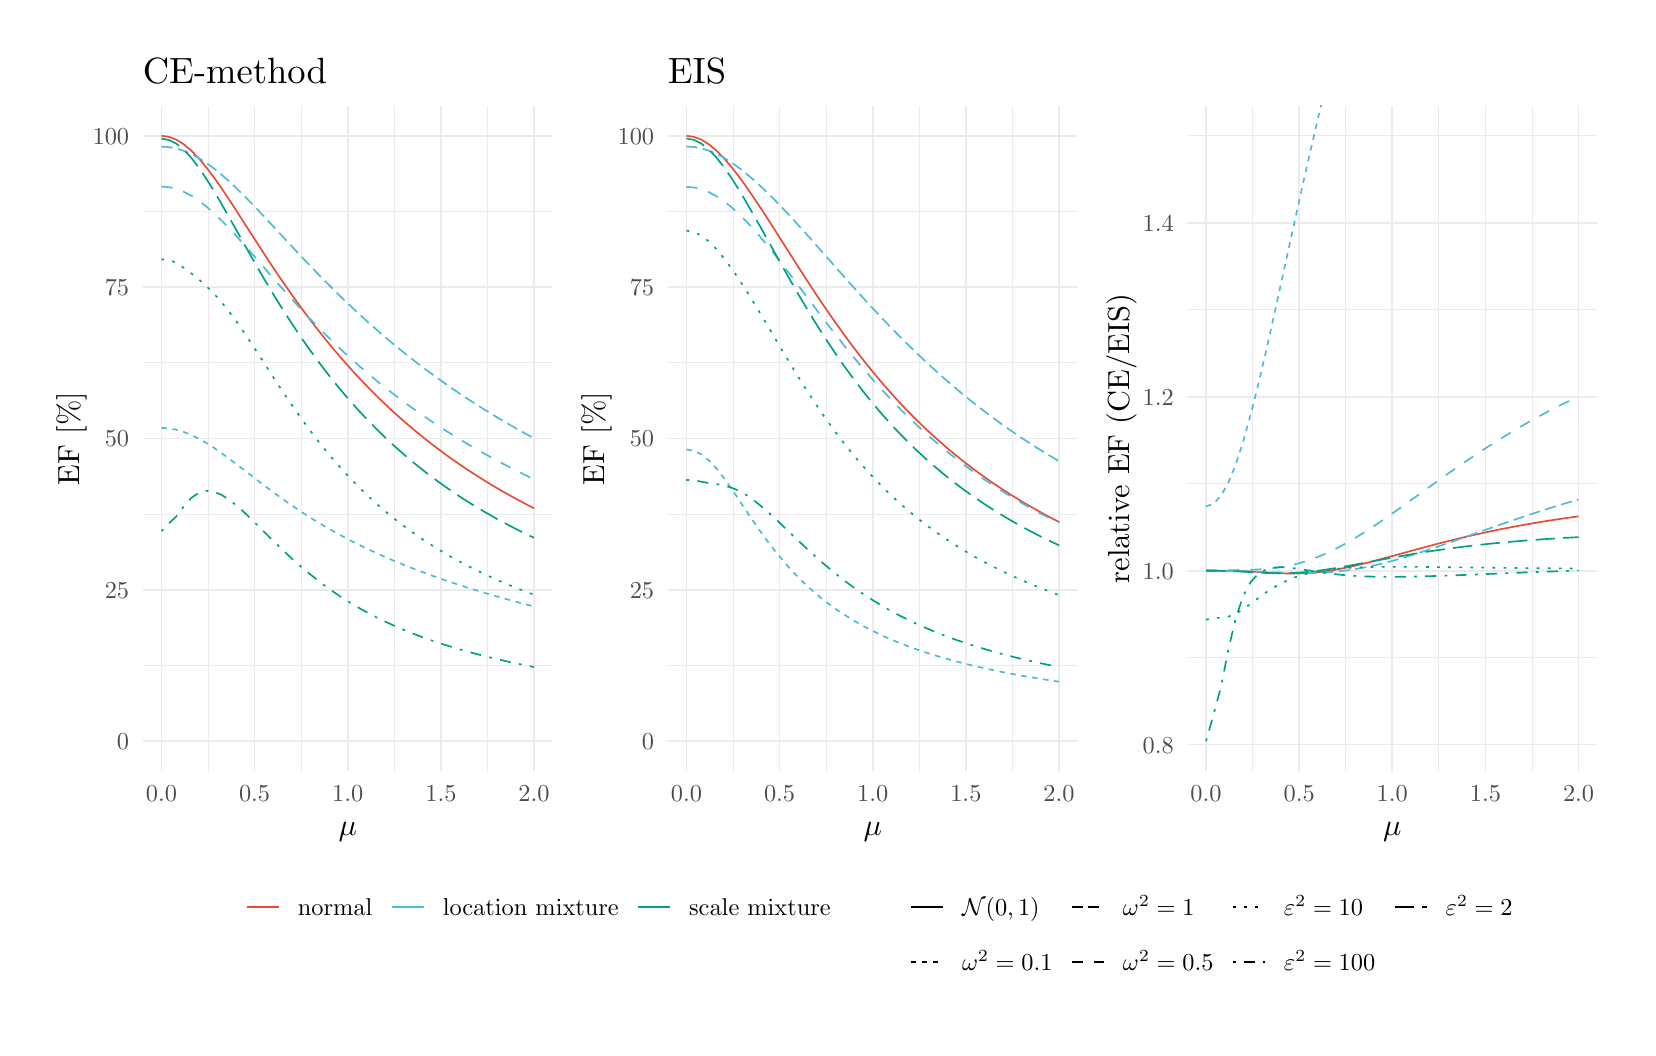
\begin{tikzpicture}[x=1pt,y=1pt]
\definecolor{fillColor}{RGB}{255,255,255}
\path[use as bounding box,fill=fillColor,fill opacity=0.00] (0,0) rectangle (578.16,361.35);
\begin{scope}
\path[clip] ( 41.61, 92.59) rectangle (189.71,333.19);
\definecolor{drawColor}{gray}{0.92}

\path[draw=drawColor,line width= 0.3pt,line join=round] ( 41.61,130.87) --
	(189.71,130.87);

\path[draw=drawColor,line width= 0.3pt,line join=round] ( 41.61,185.55) --
	(189.71,185.55);

\path[draw=drawColor,line width= 0.3pt,line join=round] ( 41.61,240.23) --
	(189.71,240.23);

\path[draw=drawColor,line width= 0.3pt,line join=round] ( 41.61,294.92) --
	(189.71,294.92);

\path[draw=drawColor,line width= 0.3pt,line join=round] ( 65.17, 92.59) --
	( 65.17,333.19);

\path[draw=drawColor,line width= 0.3pt,line join=round] ( 98.83, 92.59) --
	( 98.83,333.19);

\path[draw=drawColor,line width= 0.3pt,line join=round] (132.49, 92.59) --
	(132.49,333.19);

\path[draw=drawColor,line width= 0.3pt,line join=round] (166.14, 92.59) --
	(166.14,333.19);

\path[draw=drawColor,line width= 0.6pt,line join=round] ( 41.61,103.53) --
	(189.71,103.53);

\path[draw=drawColor,line width= 0.6pt,line join=round] ( 41.61,158.21) --
	(189.71,158.21);

\path[draw=drawColor,line width= 0.6pt,line join=round] ( 41.61,212.89) --
	(189.71,212.89);

\path[draw=drawColor,line width= 0.6pt,line join=round] ( 41.61,267.57) --
	(189.71,267.57);

\path[draw=drawColor,line width= 0.6pt,line join=round] ( 41.61,322.26) --
	(189.71,322.26);

\path[draw=drawColor,line width= 0.6pt,line join=round] ( 48.34, 92.59) --
	( 48.34,333.19);

\path[draw=drawColor,line width= 0.6pt,line join=round] ( 82.00, 92.59) --
	( 82.00,333.19);

\path[draw=drawColor,line width= 0.6pt,line join=round] (115.66, 92.59) --
	(115.66,333.19);

\path[draw=drawColor,line width= 0.6pt,line join=round] (149.32, 92.59) --
	(149.32,333.19);

\path[draw=drawColor,line width= 0.6pt,line join=round] (182.97, 92.59) --
	(182.97,333.19);
\definecolor{drawColor}{RGB}{230,75,53}

\path[draw=drawColor,line width= 0.6pt,line join=round] ( 48.34,322.26) --
	( 51.04,321.91) --
	( 53.73,320.87) --
	( 56.42,319.19) --
	( 59.11,316.93) --
	( 61.81,314.15) --
	( 64.50,310.94) --
	( 67.19,307.38) --
	( 69.88,303.57) --
	( 72.58,299.56) --
	( 75.27,295.44) --
	( 77.96,291.25) --
	( 80.65,287.04) --
	( 83.35,282.85) --
	( 86.04,278.70) --
	( 88.73,274.62) --
	( 91.42,270.62) --
	( 94.12,266.72) --
	( 96.81,262.92) --
	( 99.50,259.22) --
	(102.20,255.63) --
	(104.89,252.14) --
	(107.58,248.76) --
	(110.27,245.49) --
	(112.97,242.32) --
	(115.66,239.26) --
	(118.35,236.29) --
	(121.04,233.42) --
	(123.74,230.64) --
	(126.43,227.96) --
	(129.12,225.36) --
	(131.81,222.84) --
	(134.51,220.41) --
	(137.20,218.06) --
	(139.89,215.78) --
	(142.58,213.58) --
	(145.28,211.44) --
	(147.97,209.38) --
	(150.66,207.38) --
	(153.35,205.44) --
	(156.05,203.57) --
	(158.74,201.75) --
	(161.43,199.99) --
	(164.13,198.28) --
	(166.82,196.62) --
	(169.51,195.02) --
	(172.20,193.46) --
	(174.90,191.95) --
	(177.59,190.48) --
	(180.28,189.06) --
	(182.97,187.68);
\definecolor{drawColor}{RGB}{77,187,213}

\path[draw=drawColor,line width= 0.6pt,dash pattern=on 2pt off 2pt ,line join=round] ( 48.34,216.73) --
	( 51.04,216.56) --
	( 53.73,216.07) --
	( 56.42,215.28) --
	( 59.11,214.20) --
	( 61.81,212.87) --
	( 64.50,211.33) --
	( 67.19,209.60) --
	( 69.88,207.74) --
	( 72.58,205.78) --
	( 75.27,203.75) --
	( 77.96,201.69) --
	( 80.65,199.61) --
	( 83.35,197.54) --
	( 86.04,195.50) --
	( 88.73,193.49) --
	( 91.42,191.53) --
	( 94.12,189.63) --
	( 96.81,187.79) --
	( 99.50,186.00) --
	(102.20,184.28) --
	(104.89,182.62) --
	(107.58,181.02) --
	(110.27,179.48) --
	(112.97,177.99) --
	(115.66,176.56) --
	(118.35,175.18) --
	(121.04,173.84) --
	(123.74,172.55) --
	(126.43,171.31) --
	(129.12,170.11) --
	(131.81,168.94) --
	(134.51,167.81) --
	(137.20,166.72) --
	(139.89,165.66) --
	(142.58,164.64) --
	(145.28,163.64) --
	(147.97,162.67) --
	(150.66,161.73) --
	(153.35,160.81) --
	(156.05,159.92) --
	(158.74,159.06) --
	(161.43,158.22) --
	(164.13,157.40) --
	(166.82,156.60) --
	(169.51,155.82) --
	(172.20,155.06) --
	(174.90,154.32) --
	(177.59,153.60) --
	(180.28,152.89) --
	(182.97,152.21);

\path[draw=drawColor,line width= 0.6pt,dash pattern=on 4pt off 2pt ,line join=round] ( 48.34,318.36) --
	( 51.04,318.19) --
	( 53.73,317.68) --
	( 56.42,316.84) --
	( 59.11,315.68) --
	( 61.81,314.23) --
	( 64.50,312.51) --
	( 67.19,310.55) --
	( 69.88,308.37) --
	( 72.58,306.01) --
	( 75.27,303.50) --
	( 77.96,300.86) --
	( 80.65,298.12) --
	( 83.35,295.31) --
	( 86.04,292.45) --
	( 88.73,289.56) --
	( 91.42,286.66) --
	( 94.12,283.75) --
	( 96.81,280.87) --
	( 99.50,278.00) --
	(102.20,275.17) --
	(104.89,272.38) --
	(107.58,269.64) --
	(110.27,266.94) --
	(112.97,264.30) --
	(115.66,261.71) --
	(118.35,259.17) --
	(121.04,256.69) --
	(123.74,254.26) --
	(126.43,251.89) --
	(129.12,249.58) --
	(131.81,247.31) --
	(134.51,245.10) --
	(137.20,242.94) --
	(139.89,240.84) --
	(142.58,238.78) --
	(145.28,236.76) --
	(147.97,234.80) --
	(150.66,232.88) --
	(153.35,231.00) --
	(156.05,229.17) --
	(158.74,227.38) --
	(161.43,225.63) --
	(164.13,223.92) --
	(166.82,222.25) --
	(169.51,220.62) --
	(172.20,219.02) --
	(174.90,217.46) --
	(177.59,215.93) --
	(180.28,214.43) --
	(182.97,212.97);

\path[draw=drawColor,line width= 0.6pt,dash pattern=on 4pt off 4pt ,line join=round] ( 48.34,303.92) --
	( 51.04,303.71) --
	( 53.73,303.07) --
	( 56.42,302.03) --
	( 59.11,300.61) --
	( 61.81,298.84) --
	( 64.50,296.77) --
	( 67.19,294.42) --
	( 69.88,291.85) --
	( 72.58,289.10) --
	( 75.27,286.20) --
	( 77.96,283.21) --
	( 80.65,280.15) --
	( 83.35,277.05) --
	( 86.04,273.94) --
	( 88.73,270.84) --
	( 91.42,267.76) --
	( 94.12,264.73) --
	( 96.81,261.76) --
	( 99.50,258.84) --
	(102.20,255.99) --
	(104.89,253.21) --
	(107.58,250.49) --
	(110.27,247.86) --
	(112.97,245.29) --
	(115.66,242.80) --
	(118.35,240.37) --
	(121.04,238.02) --
	(123.74,235.73) --
	(126.43,233.50) --
	(129.12,231.34) --
	(131.81,229.24) --
	(134.51,227.19) --
	(137.20,225.20) --
	(139.89,223.26) --
	(142.58,221.38) --
	(145.28,219.54) --
	(147.97,217.75) --
	(150.66,216.01) --
	(153.35,214.31) --
	(156.05,212.66) --
	(158.74,211.04) --
	(161.43,209.47) --
	(164.13,207.93) --
	(166.82,206.43) --
	(169.51,204.97) --
	(172.20,203.54) --
	(174.90,202.15) --
	(177.59,200.79) --
	(180.28,199.46) --
	(182.97,198.15);
\definecolor{drawColor}{RGB}{0,160,135}

\path[draw=drawColor,line width= 0.6pt,dash pattern=on 1pt off 3pt ,line join=round] ( 48.34,277.59) --
	( 51.04,277.55) --
	( 53.73,276.30) --
	( 56.42,274.57) --
	( 59.11,272.59) --
	( 61.81,270.43) --
	( 64.50,268.04) --
	( 67.19,265.37) --
	( 69.88,262.36) --
	( 72.58,259.03) --
	( 75.27,255.40) --
	( 77.96,251.55) --
	( 80.65,247.52) --
	( 83.35,243.40) --
	( 86.04,239.24) --
	( 88.73,235.08) --
	( 91.42,230.98) --
	( 94.12,226.96) --
	( 96.81,223.05) --
	( 99.50,219.26) --
	(102.20,215.60) --
	(104.89,212.09) --
	(107.58,208.72) --
	(110.27,205.50) --
	(112.97,202.42) --
	(115.66,199.47) --
	(118.35,196.66) --
	(121.04,193.99) --
	(123.74,191.43) --
	(126.43,188.99) --
	(129.12,186.67) --
	(131.81,184.45) --
	(134.51,182.34) --
	(137.20,180.32) --
	(139.89,178.39) --
	(142.58,176.54) --
	(145.28,174.78) --
	(147.97,173.09) --
	(150.66,171.47) --
	(153.35,169.92) --
	(156.05,168.44) --
	(158.74,167.01) --
	(161.43,165.65) --
	(164.13,164.34) --
	(166.82,163.08) --
	(169.51,161.86) --
	(172.20,160.70) --
	(174.90,159.57) --
	(177.59,158.49) --
	(180.28,157.45) --
	(182.97,156.44);

\path[draw=drawColor,line width= 0.6pt,dash pattern=on 1pt off 3pt on 4pt off 3pt ,line join=round] ( 48.34,179.42) --
	( 51.04,182.21) --
	( 53.73,184.74) --
	( 56.42,188.36) --
	( 59.11,191.40) --
	( 61.81,193.27) --
	( 64.50,193.98) --
	( 67.19,193.69) --
	( 69.88,192.62) --
	( 72.58,190.95) --
	( 75.27,188.85) --
	( 77.96,186.47) --
	( 80.65,183.91) --
	( 83.35,181.25) --
	( 86.04,178.57) --
	( 88.73,175.90) --
	( 91.42,173.29) --
	( 94.12,170.75) --
	( 96.81,168.30) --
	( 99.50,165.96) --
	(102.20,163.72) --
	(104.89,161.59) --
	(107.58,159.57) --
	(110.27,157.65) --
	(112.97,155.83) --
	(115.66,154.10) --
	(118.35,152.47) --
	(121.04,150.93) --
	(123.74,149.47) --
	(126.43,148.08) --
	(129.12,146.77) --
	(131.81,145.52) --
	(134.51,144.34) --
	(137.20,143.21) --
	(139.89,142.15) --
	(142.58,141.13) --
	(145.28,140.16) --
	(147.97,139.24) --
	(150.66,138.36) --
	(153.35,137.52) --
	(156.05,136.72) --
	(158.74,135.95) --
	(161.43,135.22) --
	(164.13,134.52) --
	(166.82,133.84) --
	(169.51,133.20) --
	(172.20,132.58) --
	(174.90,131.98) --
	(177.59,131.41) --
	(180.28,130.86) --
	(182.97,130.33);

\path[draw=drawColor,line width= 0.6pt,dash pattern=on 7pt off 3pt ,line join=round] ( 48.34,321.24) --
	( 51.04,320.79) --
	( 53.73,319.43) --
	( 56.42,317.25) --
	( 59.11,314.34) --
	( 61.81,310.83) --
	( 64.50,306.84) --
	( 67.19,302.51) --
	( 69.88,297.94) --
	( 72.58,293.22) --
	( 75.27,288.43) --
	( 77.96,283.63) --
	( 80.65,278.86) --
	( 83.35,274.17) --
	( 86.04,269.56) --
	( 88.73,265.07) --
	( 91.42,260.71) --
	( 94.12,256.47) --
	( 96.81,252.37) --
	( 99.50,248.40) --
	(102.20,244.58) --
	(104.89,240.89) --
	(107.58,237.34) --
	(110.27,233.92) --
	(112.97,230.62) --
	(115.66,227.45) --
	(118.35,224.40) --
	(121.04,221.47) --
	(123.74,218.65) --
	(126.43,215.93) --
	(129.12,213.32) --
	(131.81,210.81) --
	(134.51,208.39) --
	(137.20,206.06) --
	(139.89,203.82) --
	(142.58,201.66) --
	(145.28,199.58) --
	(147.97,197.58) --
	(150.66,195.64) --
	(153.35,193.78) --
	(156.05,191.98) --
	(158.74,190.24) --
	(161.43,188.57) --
	(164.13,186.95) --
	(166.82,185.39) --
	(169.51,183.87) --
	(172.20,182.41) --
	(174.90,181.00) --
	(177.59,179.63) --
	(180.28,178.31) --
	(182.97,177.02);
\end{scope}
\begin{scope}
\path[clip] (  0.00,  0.00) rectangle (578.16,361.35);
\definecolor{drawColor}{gray}{0.30}

\node[text=drawColor,anchor=base east,inner sep=0pt, outer sep=0pt, scale=  0.88] at ( 36.66,100.50) {0};

\node[text=drawColor,anchor=base east,inner sep=0pt, outer sep=0pt, scale=  0.88] at ( 36.66,155.18) {25};

\node[text=drawColor,anchor=base east,inner sep=0pt, outer sep=0pt, scale=  0.88] at ( 36.66,209.86) {50};

\node[text=drawColor,anchor=base east,inner sep=0pt, outer sep=0pt, scale=  0.88] at ( 36.66,264.54) {75};

\node[text=drawColor,anchor=base east,inner sep=0pt, outer sep=0pt, scale=  0.88] at ( 36.66,319.23) {100};
\end{scope}
\begin{scope}
\path[clip] (  0.00,  0.00) rectangle (578.16,361.35);
\definecolor{drawColor}{gray}{0.30}

\node[text=drawColor,anchor=base,inner sep=0pt, outer sep=0pt, scale=  0.88] at ( 48.34, 81.58) {0.0};

\node[text=drawColor,anchor=base,inner sep=0pt, outer sep=0pt, scale=  0.88] at ( 82.00, 81.58) {0.5};

\node[text=drawColor,anchor=base,inner sep=0pt, outer sep=0pt, scale=  0.88] at (115.66, 81.58) {1.0};

\node[text=drawColor,anchor=base,inner sep=0pt, outer sep=0pt, scale=  0.88] at (149.32, 81.58) {1.5};

\node[text=drawColor,anchor=base,inner sep=0pt, outer sep=0pt, scale=  0.88] at (182.97, 81.58) {2.0};
\end{scope}
\begin{scope}
\path[clip] (  0.00,  0.00) rectangle (578.16,361.35);
\definecolor{drawColor}{RGB}{0,0,0}

\node[text=drawColor,anchor=base,inner sep=0pt, outer sep=0pt, scale=  1.10] at (115.66, 69.55) {$\mu$};
\end{scope}
\begin{scope}
\path[clip] (  0.00,  0.00) rectangle (578.16,361.35);
\definecolor{drawColor}{RGB}{0,0,0}

\node[text=drawColor,rotate= 90.00,anchor=base,inner sep=0pt, outer sep=0pt, scale=  1.10] at ( 18.58,212.89) {EF [\%]};
\end{scope}
\begin{scope}
\path[clip] (  0.00,  0.00) rectangle (578.16,361.35);
\definecolor{drawColor}{RGB}{0,0,0}

\node[text=drawColor,anchor=base west,inner sep=0pt, outer sep=0pt, scale=  1.32] at ( 41.61,341.26) {CE-method};
\end{scope}
\begin{scope}
\path[clip] (231.32, 92.59) rectangle (379.41,333.19);
\definecolor{drawColor}{gray}{0.92}

\path[draw=drawColor,line width= 0.3pt,line join=round] (231.32,130.87) --
	(379.41,130.87);

\path[draw=drawColor,line width= 0.3pt,line join=round] (231.32,185.55) --
	(379.41,185.55);

\path[draw=drawColor,line width= 0.3pt,line join=round] (231.32,240.23) --
	(379.41,240.23);

\path[draw=drawColor,line width= 0.3pt,line join=round] (231.32,294.92) --
	(379.41,294.92);

\path[draw=drawColor,line width= 0.3pt,line join=round] (254.88, 92.59) --
	(254.88,333.19);

\path[draw=drawColor,line width= 0.3pt,line join=round] (288.53, 92.59) --
	(288.53,333.19);

\path[draw=drawColor,line width= 0.3pt,line join=round] (322.19, 92.59) --
	(322.19,333.19);

\path[draw=drawColor,line width= 0.3pt,line join=round] (355.85, 92.59) --
	(355.85,333.19);

\path[draw=drawColor,line width= 0.6pt,line join=round] (231.32,103.53) --
	(379.41,103.53);

\path[draw=drawColor,line width= 0.6pt,line join=round] (231.32,158.21) --
	(379.41,158.21);

\path[draw=drawColor,line width= 0.6pt,line join=round] (231.32,212.89) --
	(379.41,212.89);

\path[draw=drawColor,line width= 0.6pt,line join=round] (231.32,267.57) --
	(379.41,267.57);

\path[draw=drawColor,line width= 0.6pt,line join=round] (231.32,322.26) --
	(379.41,322.26);

\path[draw=drawColor,line width= 0.6pt,line join=round] (238.05, 92.59) --
	(238.05,333.19);

\path[draw=drawColor,line width= 0.6pt,line join=round] (271.71, 92.59) --
	(271.71,333.19);

\path[draw=drawColor,line width= 0.6pt,line join=round] (305.36, 92.59) --
	(305.36,333.19);

\path[draw=drawColor,line width= 0.6pt,line join=round] (339.02, 92.59) --
	(339.02,333.19);

\path[draw=drawColor,line width= 0.6pt,line join=round] (372.68, 92.59) --
	(372.68,333.19);
\definecolor{drawColor}{RGB}{230,75,53}

\path[draw=drawColor,line width= 0.6pt,line join=round] (238.05,322.26) --
	(240.74,321.91) --
	(243.43,320.88) --
	(246.13,319.21) --
	(248.82,316.98) --
	(251.51,314.26) --
	(254.20,311.14) --
	(256.90,307.68) --
	(259.59,303.97) --
	(262.28,300.06) --
	(264.97,296.01) --
	(267.67,291.85) --
	(270.36,287.64) --
	(273.05,283.39) --
	(275.74,279.15) --
	(278.44,274.92) --
	(281.13,270.74) --
	(283.82,266.62) --
	(286.51,262.58) --
	(289.21,258.62) --
	(291.90,254.75) --
	(294.59,250.99) --
	(297.29,247.33) --
	(299.98,243.78) --
	(302.67,240.34) --
	(305.36,237.01) --
	(308.06,233.79) --
	(310.75,230.68) --
	(313.44,227.67) --
	(316.13,224.77) --
	(318.83,221.98) --
	(321.52,219.28) --
	(324.21,216.68) --
	(326.90,214.17) --
	(329.60,211.76) --
	(332.29,209.42) --
	(334.98,207.18) --
	(337.67,205.01) --
	(340.37,202.91) --
	(343.06,200.89) --
	(345.75,198.95) --
	(348.44,197.06) --
	(351.14,195.25) --
	(353.83,193.49) --
	(356.52,191.80) --
	(359.22,190.16) --
	(361.91,188.57) --
	(364.60,187.04) --
	(367.29,185.55) --
	(369.99,184.12) --
	(372.68,182.72);
\definecolor{drawColor}{RGB}{77,187,213}

\path[draw=drawColor,line width= 0.6pt,dash pattern=on 2pt off 2pt ,line join=round] (238.05,208.92) --
	(240.74,208.49) --
	(243.43,207.16) --
	(246.13,204.99) --
	(248.82,202.12) --
	(251.51,198.70) --
	(254.20,194.90) --
	(256.90,190.91) --
	(259.59,186.86) --
	(262.28,182.87) --
	(264.97,179.02) --
	(267.67,175.34) --
	(270.36,171.87) --
	(273.05,168.61) --
	(275.74,165.57) --
	(278.44,162.75) --
	(281.13,160.12) --
	(283.82,157.68) --
	(286.51,155.41) --
	(289.21,153.30) --
	(291.90,151.35) --
	(294.59,149.52) --
	(297.29,147.82) --
	(299.98,146.23) --
	(302.67,144.75) --
	(305.36,143.36) --
	(308.06,142.05) --
	(310.75,140.83) --
	(313.44,139.67) --
	(316.13,138.59) --
	(318.83,137.57) --
	(321.52,136.60) --
	(324.21,135.69) --
	(326.90,134.82) --
	(329.60,134.00) --
	(332.29,133.22) --
	(334.98,132.48) --
	(337.67,131.78) --
	(340.37,131.11) --
	(343.06,130.47) --
	(345.75,129.86) --
	(348.44,129.28) --
	(351.14,128.72) --
	(353.83,128.19) --
	(356.52,127.68) --
	(359.22,127.19) --
	(361.91,126.72) --
	(364.60,126.26) --
	(367.29,125.84) --
	(369.99,125.41) --
	(372.68,125.02);

\path[draw=drawColor,line width= 0.6pt,dash pattern=on 4pt off 2pt ,line join=round] (238.05,318.39) --
	(240.74,318.23) --
	(243.43,317.72) --
	(246.13,316.90) --
	(248.82,315.77) --
	(251.51,314.36) --
	(254.20,312.69) --
	(256.90,310.78) --
	(259.59,308.67) --
	(262.28,306.38) --
	(264.97,303.93) --
	(267.67,301.34) --
	(270.36,298.64) --
	(273.05,295.84) --
	(275.74,292.97) --
	(278.44,290.02) --
	(281.13,287.04) --
	(283.82,284.02) --
	(286.51,280.97) --
	(289.21,277.92) --
	(291.90,274.87) --
	(294.59,271.83) --
	(297.29,268.81) --
	(299.98,265.82) --
	(302.67,262.86) --
	(305.36,259.94) --
	(308.06,257.07) --
	(310.75,254.24) --
	(313.44,251.47) --
	(316.13,248.75) --
	(318.83,246.09) --
	(321.52,243.48) --
	(324.21,240.93) --
	(326.90,238.45) --
	(329.60,236.02) --
	(332.29,233.65) --
	(334.98,231.34) --
	(337.67,229.09) --
	(340.37,226.90) --
	(343.06,224.76) --
	(345.75,222.68) --
	(348.44,220.65) --
	(351.14,218.68) --
	(353.83,216.76) --
	(356.52,214.89) --
	(359.22,213.08) --
	(361.91,211.31) --
	(364.60,209.58) --
	(367.29,207.91) --
	(369.99,206.28) --
	(372.68,204.69);

\path[draw=drawColor,line width= 0.6pt,dash pattern=on 4pt off 4pt ,line join=round] (238.05,303.81) --
	(240.74,303.60) --
	(243.43,302.96) --
	(246.13,301.91) --
	(248.82,300.48) --
	(251.51,298.68) --
	(254.20,296.56) --
	(256.90,294.14) --
	(259.59,291.47) --
	(262.28,288.56) --
	(264.97,285.47) --
	(267.67,282.21) --
	(270.36,278.83) --
	(273.05,275.35) --
	(275.74,271.81) --
	(278.44,268.23) --
	(281.13,264.63) --
	(283.82,261.04) --
	(286.51,257.47) --
	(289.21,253.94) --
	(291.90,250.47) --
	(294.59,247.06) --
	(297.29,243.72) --
	(299.98,240.46) --
	(302.67,237.28) --
	(305.36,234.20) --
	(308.06,231.19) --
	(310.75,228.29) --
	(313.44,225.47) --
	(316.13,222.73) --
	(318.83,220.09) --
	(321.52,217.53) --
	(324.21,215.06) --
	(326.90,212.68) --
	(329.60,210.37) --
	(332.29,208.14) --
	(334.98,205.99) --
	(337.67,203.90) --
	(340.37,201.90) --
	(343.06,199.95) --
	(345.75,198.07) --
	(348.44,196.26) --
	(351.14,194.50) --
	(353.83,192.81) --
	(356.52,191.16) --
	(359.22,189.58) --
	(361.91,188.04) --
	(364.60,186.55) --
	(367.29,185.11) --
	(369.99,183.71) --
	(372.68,182.36);
\definecolor{drawColor}{RGB}{0,160,135}

\path[draw=drawColor,line width= 0.6pt,dash pattern=on 1pt off 3pt ,line join=round] (238.05,287.99) --
	(240.74,287.55) --
	(243.43,286.21) --
	(246.13,284.10) --
	(248.82,281.37) --
	(251.51,278.15) --
	(254.20,274.54) --
	(256.90,270.63) --
	(259.59,266.48) --
	(262.28,262.15) --
	(264.97,257.68) --
	(267.67,253.15) --
	(270.36,248.59) --
	(273.05,244.05) --
	(275.74,239.56) --
	(278.44,235.17) --
	(281.13,230.89) --
	(283.82,226.75) --
	(286.51,222.74) --
	(289.21,218.89) --
	(291.90,215.20) --
	(294.59,211.67) --
	(297.29,208.29) --
	(299.98,205.06) --
	(302.67,201.98) --
	(305.36,199.05) --
	(308.06,196.25) --
	(310.75,193.59) --
	(313.44,191.05) --
	(316.13,188.63) --
	(318.83,186.32) --
	(321.52,184.12) --
	(324.21,182.02) --
	(326.90,180.01) --
	(329.60,178.10) --
	(332.29,176.27) --
	(334.98,174.52) --
	(337.67,172.84) --
	(340.37,171.24) --
	(343.06,169.70) --
	(345.75,168.23) --
	(348.44,166.81) --
	(351.14,165.46) --
	(353.83,164.15) --
	(356.52,162.90) --
	(359.22,161.70) --
	(361.91,160.54) --
	(364.60,159.42) --
	(367.29,158.35) --
	(369.99,157.31) --
	(372.68,156.31);

\path[draw=drawColor,line width= 0.6pt,dash pattern=on 1pt off 3pt on 4pt off 3pt ,line join=round] (238.05,197.92) --
	(240.74,197.81) --
	(243.43,197.28) --
	(246.13,196.80) --
	(248.82,196.42) --
	(251.51,195.94) --
	(254.20,195.16) --
	(256.90,194.02) --
	(259.59,192.50) --
	(262.28,190.64) --
	(264.97,188.51) --
	(267.67,186.18) --
	(270.36,183.71) --
	(273.05,181.16) --
	(275.74,178.58) --
	(278.44,176.01) --
	(281.13,173.47) --
	(283.82,171.00) --
	(286.51,168.60) --
	(289.21,166.30) --
	(291.90,164.08) --
	(294.59,161.96) --
	(297.29,159.95) --
	(299.98,158.02) --
	(302.67,156.20) --
	(305.36,154.47) --
	(308.06,152.82) --
	(310.75,151.26) --
	(313.44,149.78) --
	(316.13,148.37) --
	(318.83,147.04) --
	(321.52,145.78) --
	(324.21,144.57) --
	(326.90,143.43) --
	(329.60,142.34) --
	(332.29,141.31) --
	(334.98,140.32) --
	(337.67,139.39) --
	(340.37,138.49) --
	(343.06,137.64) --
	(345.75,136.82) --
	(348.44,136.04) --
	(351.14,135.29) --
	(353.83,134.58) --
	(356.52,133.89) --
	(359.22,133.24) --
	(361.91,132.61) --
	(364.60,132.00) --
	(367.29,131.42) --
	(369.99,130.86) --
	(372.68,130.33);

\path[draw=drawColor,line width= 0.6pt,dash pattern=on 7pt off 3pt ,line join=round] (238.05,321.27) --
	(240.74,320.81) --
	(243.43,319.47) --
	(246.13,317.33) --
	(248.82,314.48) --
	(251.51,311.06) --
	(254.20,307.17) --
	(256.90,302.94) --
	(259.59,298.44) --
	(262.28,293.77) --
	(264.97,288.99) --
	(267.67,284.15) --
	(270.36,279.31) --
	(273.05,274.50) --
	(275.74,269.75) --
	(278.44,265.08) --
	(281.13,260.53) --
	(283.82,256.09) --
	(286.51,251.79) --
	(289.21,247.62) --
	(291.90,243.60) --
	(294.59,239.72) --
	(297.29,235.98) --
	(299.98,232.39) --
	(302.67,228.93) --
	(305.36,225.62) --
	(308.06,222.43) --
	(310.75,219.38) --
	(313.44,216.45) --
	(316.13,213.63) --
	(318.83,210.94) --
	(321.52,208.35) --
	(324.21,205.86) --
	(326.90,203.48) --
	(329.60,201.18) --
	(332.29,198.98) --
	(334.98,196.87) --
	(337.67,194.84) --
	(340.37,192.88) --
	(343.06,191.00) --
	(345.75,189.19) --
	(348.44,187.45) --
	(351.14,185.77) --
	(353.83,184.15) --
	(356.52,182.59) --
	(359.22,181.08) --
	(361.91,179.63) --
	(364.60,178.23) --
	(367.29,176.87) --
	(369.99,175.56) --
	(372.68,174.29);
\end{scope}
\begin{scope}
\path[clip] (  0.00,  0.00) rectangle (578.16,361.35);
\definecolor{drawColor}{gray}{0.30}

\node[text=drawColor,anchor=base east,inner sep=0pt, outer sep=0pt, scale=  0.88] at (226.37,100.50) {0};

\node[text=drawColor,anchor=base east,inner sep=0pt, outer sep=0pt, scale=  0.88] at (226.37,155.18) {25};

\node[text=drawColor,anchor=base east,inner sep=0pt, outer sep=0pt, scale=  0.88] at (226.37,209.86) {50};

\node[text=drawColor,anchor=base east,inner sep=0pt, outer sep=0pt, scale=  0.88] at (226.37,264.54) {75};

\node[text=drawColor,anchor=base east,inner sep=0pt, outer sep=0pt, scale=  0.88] at (226.37,319.23) {100};
\end{scope}
\begin{scope}
\path[clip] (  0.00,  0.00) rectangle (578.16,361.35);
\definecolor{drawColor}{gray}{0.30}

\node[text=drawColor,anchor=base,inner sep=0pt, outer sep=0pt, scale=  0.88] at (238.05, 81.58) {0.0};

\node[text=drawColor,anchor=base,inner sep=0pt, outer sep=0pt, scale=  0.88] at (271.71, 81.58) {0.5};

\node[text=drawColor,anchor=base,inner sep=0pt, outer sep=0pt, scale=  0.88] at (305.36, 81.58) {1.0};

\node[text=drawColor,anchor=base,inner sep=0pt, outer sep=0pt, scale=  0.88] at (339.02, 81.58) {1.5};

\node[text=drawColor,anchor=base,inner sep=0pt, outer sep=0pt, scale=  0.88] at (372.68, 81.58) {2.0};
\end{scope}
\begin{scope}
\path[clip] (  0.00,  0.00) rectangle (578.16,361.35);
\definecolor{drawColor}{RGB}{0,0,0}

\node[text=drawColor,anchor=base,inner sep=0pt, outer sep=0pt, scale=  1.10] at (305.36, 69.55) {$\mu$};
\end{scope}
\begin{scope}
\path[clip] (  0.00,  0.00) rectangle (578.16,361.35);
\definecolor{drawColor}{RGB}{0,0,0}

\node[text=drawColor,rotate= 90.00,anchor=base,inner sep=0pt, outer sep=0pt, scale=  1.10] at (208.28,212.89) {EF [\%]};
\end{scope}
\begin{scope}
\path[clip] (  0.00,  0.00) rectangle (578.16,361.35);
\definecolor{drawColor}{RGB}{0,0,0}

\node[text=drawColor,anchor=base west,inner sep=0pt, outer sep=0pt, scale=  1.32] at (231.32,341.26) {EIS};
\end{scope}
\begin{scope}
\path[clip] (419.07, 92.59) rectangle (567.16,333.19);
\definecolor{drawColor}{gray}{0.92}

\path[draw=drawColor,line width= 0.3pt,line join=round] (419.07,133.70) --
	(567.16,133.70);

\path[draw=drawColor,line width= 0.3pt,line join=round] (419.07,196.55) --
	(567.16,196.55);

\path[draw=drawColor,line width= 0.3pt,line join=round] (419.07,259.40) --
	(567.16,259.40);

\path[draw=drawColor,line width= 0.3pt,line join=round] (419.07,322.26) --
	(567.16,322.26);

\path[draw=drawColor,line width= 0.3pt,line join=round] (442.63, 92.59) --
	(442.63,333.19);

\path[draw=drawColor,line width= 0.3pt,line join=round] (476.28, 92.59) --
	(476.28,333.19);

\path[draw=drawColor,line width= 0.3pt,line join=round] (509.94, 92.59) --
	(509.94,333.19);

\path[draw=drawColor,line width= 0.3pt,line join=round] (543.60, 92.59) --
	(543.60,333.19);

\path[draw=drawColor,line width= 0.6pt,line join=round] (419.07,102.27) --
	(567.16,102.27);

\path[draw=drawColor,line width= 0.6pt,line join=round] (419.07,165.12) --
	(567.16,165.12);

\path[draw=drawColor,line width= 0.6pt,line join=round] (419.07,227.98) --
	(567.16,227.98);

\path[draw=drawColor,line width= 0.6pt,line join=round] (419.07,290.83) --
	(567.16,290.83);

\path[draw=drawColor,line width= 0.6pt,line join=round] (425.80, 92.59) --
	(425.80,333.19);

\path[draw=drawColor,line width= 0.6pt,line join=round] (459.46, 92.59) --
	(459.46,333.19);

\path[draw=drawColor,line width= 0.6pt,line join=round] (493.11, 92.59) --
	(493.11,333.19);

\path[draw=drawColor,line width= 0.6pt,line join=round] (526.77, 92.59) --
	(526.77,333.19);

\path[draw=drawColor,line width= 0.6pt,line join=round] (560.43, 92.59) --
	(560.43,333.19);
\definecolor{drawColor}{RGB}{230,75,53}

\path[draw=drawColor,line width= 0.6pt,line join=round] (425.80,165.12) --
	(428.49,165.12) --
	(431.18,165.12) --
	(433.88,165.10) --
	(436.57,165.04) --
	(439.26,164.95) --
	(441.95,164.82) --
	(444.65,164.66) --
	(447.34,164.49) --
	(450.03,164.33) --
	(452.72,164.19) --
	(455.42,164.11) --
	(458.11,164.10) --
	(460.80,164.17) --
	(463.49,164.33) --
	(466.19,164.57) --
	(468.88,164.90) --
	(471.57,165.31) --
	(474.26,165.80) --
	(476.96,166.34) --
	(479.65,166.94) --
	(482.34,167.58) --
	(485.04,168.26) --
	(487.73,168.97) --
	(490.42,169.69) --
	(493.11,170.42) --
	(495.81,171.16) --
	(498.50,171.90) --
	(501.19,172.64) --
	(503.88,173.37) --
	(506.58,174.09) --
	(509.27,174.80) --
	(511.96,175.49) --
	(514.65,176.16) --
	(517.35,176.81) --
	(520.04,177.45) --
	(522.73,178.07) --
	(525.42,178.67) --
	(528.12,179.25) --
	(530.81,179.81) --
	(533.50,180.35) --
	(536.19,180.87) --
	(538.89,181.37) --
	(541.58,181.85) --
	(544.27,182.32) --
	(546.97,182.77) --
	(549.66,183.20) --
	(552.35,183.62) --
	(555.04,184.02) --
	(557.74,184.40) --
	(560.43,184.77);
\definecolor{drawColor}{RGB}{77,187,213}

\path[draw=drawColor,line width= 0.6pt,dash pattern=on 2pt off 2pt ,line join=round] (425.80,188.40) --
	(428.49,189.29) --
	(431.18,192.17) --
	(433.88,196.98) --
	(436.57,203.63) --
	(439.26,211.93) --
	(441.95,221.60) --
	(444.65,232.35) --
	(447.34,243.86) --
	(450.03,255.86) --
	(452.72,268.11) --
	(455.42,280.44) --
	(458.11,292.70) --
	(460.80,304.82) --
	(463.49,316.68) --
	(466.19,328.29) --
	(468.88,339.58) --
	(471.57,350.57) --
	(474.26,361.23) --
	(476.96,371.58) --
	(479.65,381.61) --
	(482.34,391.32) --
	(485.04,400.71) --
	(487.73,409.83) --
	(490.42,418.62) --
	(493.11,427.13) --
	(495.81,435.33) --
	(498.50,443.27) --
	(501.19,451.00) --
	(503.88,458.41) --
	(506.58,465.52) --
	(509.27,472.43) --
	(511.96,479.03) --
	(514.65,485.44) --
	(517.35,491.62) --
	(520.04,497.59) --
	(522.73,503.30) --
	(525.42,508.74) --
	(528.12,514.01) --
	(530.81,519.13) --
	(533.50,524.04) --
	(536.19,528.56) --
	(538.89,533.09) --
	(541.58,537.38) --
	(544.27,541.48) --
	(546.97,545.45) --
	(549.66,549.09) --
	(552.35,552.97) --
	(555.04,555.99) --
	(557.74,559.72) --
	(560.43,562.80);

\path[draw=drawColor,line width= 0.6pt,dash pattern=on 4pt off 2pt ,line join=round] (425.80,165.08) --
	(428.49,165.07) --
	(431.18,165.06) --
	(433.88,165.03) --
	(436.57,164.99) --
	(439.26,164.94) --
	(441.95,164.86) --
	(444.65,164.77) --
	(447.34,164.66) --
	(450.03,164.55) --
	(452.72,164.45) --
	(455.42,164.36) --
	(458.11,164.29) --
	(460.80,164.26) --
	(463.49,164.27) --
	(466.19,164.34) --
	(468.88,164.47) --
	(471.57,164.67) --
	(474.26,164.94) --
	(476.96,165.28) --
	(479.65,165.68) --
	(482.34,166.16) --
	(485.04,166.70) --
	(487.73,167.30) --
	(490.42,167.96) --
	(493.11,168.67) --
	(495.81,169.43) --
	(498.50,170.23) --
	(501.19,171.06) --
	(503.88,171.92) --
	(506.58,172.82) --
	(509.27,173.73) --
	(511.96,174.66) --
	(514.65,175.60) --
	(517.35,176.55) --
	(520.04,177.51) --
	(522.73,178.46) --
	(525.42,179.42) --
	(528.12,180.37) --
	(530.81,181.31) --
	(533.50,182.25) --
	(536.19,183.18) --
	(538.89,184.09) --
	(541.58,185.00) --
	(544.27,185.89) --
	(546.97,186.76) --
	(549.66,187.61) --
	(552.35,188.45) --
	(555.04,189.28) --
	(557.74,190.08) --
	(560.43,190.87);

\path[draw=drawColor,line width= 0.6pt,dash pattern=on 4pt off 4pt ,line join=round] (425.80,165.29) --
	(428.49,165.30) --
	(431.18,165.30) --
	(433.88,165.32) --
	(436.57,165.34) --
	(439.26,165.39) --
	(441.95,165.46) --
	(444.65,165.58) --
	(447.34,165.77) --
	(450.03,166.04) --
	(452.72,166.40) --
	(455.42,166.88) --
	(458.11,167.49) --
	(460.80,168.23) --
	(463.49,169.10) --
	(466.19,170.11) --
	(468.88,171.24) --
	(471.57,172.50) --
	(474.26,173.88) --
	(476.96,175.36) --
	(479.65,176.93) --
	(482.34,178.59) --
	(485.04,180.31) --
	(487.73,182.10) --
	(490.42,183.94) --
	(493.11,185.81) --
	(495.81,187.72) --
	(498.50,189.64) --
	(501.19,191.57) --
	(503.88,193.51) --
	(506.58,195.45) --
	(509.27,197.38) --
	(511.96,199.29) --
	(514.65,201.19) --
	(517.35,203.05) --
	(520.04,204.90) --
	(522.73,206.70) --
	(525.42,208.49) --
	(528.12,210.22) --
	(530.81,211.94) --
	(533.50,213.61) --
	(536.19,215.24) --
	(538.89,216.83) --
	(541.58,218.38) --
	(544.27,219.89) --
	(546.97,221.36) --
	(549.66,222.79) --
	(552.35,224.17) --
	(555.04,225.52) --
	(557.74,226.83) --
	(560.43,228.10);
\definecolor{drawColor}{RGB}{0,160,135}

\path[draw=drawColor,line width= 0.6pt,dash pattern=on 1pt off 3pt ,line join=round] (425.80,147.41) --
	(428.49,148.05) --
	(431.18,148.08) --
	(433.88,148.53) --
	(436.57,149.60) --
	(439.26,151.23) --
	(441.95,153.18) --
	(444.65,155.22) --
	(447.34,157.18) --
	(450.03,158.94) --
	(452.72,160.47) --
	(455.42,161.76) --
	(458.11,162.82) --
	(460.80,163.68) --
	(463.49,164.37) --
	(466.19,164.91) --
	(468.88,165.34) --
	(471.57,165.67) --
	(474.26,165.92) --
	(476.96,166.12) --
	(479.65,166.26) --
	(482.34,166.36) --
	(485.04,166.43) --
	(487.73,166.48) --
	(490.42,166.51) --
	(493.11,166.52) --
	(495.81,166.52) --
	(498.50,166.51) --
	(501.19,166.50) --
	(503.88,166.48) --
	(506.58,166.46) --
	(509.27,166.43) --
	(511.96,166.40) --
	(514.65,166.37) --
	(517.35,166.34) --
	(520.04,166.31) --
	(522.73,166.28) --
	(525.42,166.25) --
	(528.12,166.22) --
	(530.81,166.19) --
	(533.50,166.16) --
	(536.19,166.13) --
	(538.89,166.10) --
	(541.58,166.07) --
	(544.27,166.05) --
	(546.97,166.02) --
	(549.66,166.00) --
	(552.35,165.97) --
	(555.04,165.95) --
	(557.74,165.93) --
	(560.43,165.90);

\path[draw=drawColor,line width= 0.6pt,dash pattern=on 1pt off 3pt on 4pt off 3pt ,line join=round] (425.80,103.53) --
	(428.49,113.12) --
	(431.18,123.09) --
	(433.88,136.69) --
	(436.57,148.14) --
	(439.26,156.07) --
	(441.95,161.07) --
	(444.65,163.98) --
	(447.34,165.54) --
	(450.03,166.23) --
	(452.72,166.39) --
	(455.42,166.24) --
	(458.11,165.92) --
	(460.80,165.52) --
	(463.49,165.09) --
	(466.19,164.67) --
	(468.88,164.29) --
	(471.57,163.96) --
	(474.26,163.67) --
	(476.96,163.44) --
	(479.65,163.25) --
	(482.34,163.11) --
	(485.04,163.01) --
	(487.73,162.94) --
	(490.42,162.91) --
	(493.11,162.90) --
	(495.81,162.91) --
	(498.50,162.95) --
	(501.19,163.00) --
	(503.88,163.07) --
	(506.58,163.14) --
	(509.27,163.23) --
	(511.96,163.32) --
	(514.65,163.42) --
	(517.35,163.52) --
	(520.04,163.63) --
	(522.73,163.74) --
	(525.42,163.85) --
	(528.12,163.96) --
	(530.81,164.07) --
	(533.50,164.17) --
	(536.19,164.28) --
	(538.89,164.39) --
	(541.58,164.50) --
	(544.27,164.60) --
	(546.97,164.70) --
	(549.66,164.80) --
	(552.35,164.90) --
	(555.04,165.00) --
	(557.74,165.10) --
	(560.43,165.19);

\path[draw=drawColor,line width= 0.6pt,dash pattern=on 7pt off 3pt ,line join=round] (425.80,165.08) --
	(428.49,165.09) --
	(431.18,165.06) --
	(433.88,165.00) --
	(436.57,164.91) --
	(439.26,164.77) --
	(441.95,164.61) --
	(444.65,164.45) --
	(447.34,164.31) --
	(450.03,164.22) --
	(452.72,164.18) --
	(455.42,164.22) --
	(458.11,164.33) --
	(460.80,164.52) --
	(463.49,164.78) --
	(466.19,165.10) --
	(468.88,165.48) --
	(471.57,165.90) --
	(474.26,166.35) --
	(476.96,166.83) --
	(479.65,167.33) --
	(482.34,167.84) --
	(485.04,168.34) --
	(487.73,168.85) --
	(490.42,169.35) --
	(493.11,169.85) --
	(495.81,170.33) --
	(498.50,170.80) --
	(501.19,171.25) --
	(503.88,171.69) --
	(506.58,172.11) --
	(509.27,172.51) --
	(511.96,172.89) --
	(514.65,173.26) --
	(517.35,173.61) --
	(520.04,173.94) --
	(522.73,174.26) --
	(525.42,174.56) --
	(528.12,174.84) --
	(530.81,175.11) --
	(533.50,175.36) --
	(536.19,175.60) --
	(538.89,175.83) --
	(541.58,176.05) --
	(544.27,176.25) --
	(546.97,176.44) --
	(549.66,176.63) --
	(552.35,176.79) --
	(555.04,176.96) --
	(557.74,177.11) --
	(560.43,177.25);
\end{scope}
\begin{scope}
\path[clip] (  0.00,  0.00) rectangle (578.16,361.35);
\definecolor{drawColor}{gray}{0.30}

\node[text=drawColor,anchor=base east,inner sep=0pt, outer sep=0pt, scale=  0.88] at (414.12, 99.24) {0.8};

\node[text=drawColor,anchor=base east,inner sep=0pt, outer sep=0pt, scale=  0.88] at (414.12,162.09) {1.0};

\node[text=drawColor,anchor=base east,inner sep=0pt, outer sep=0pt, scale=  0.88] at (414.12,224.95) {1.2};

\node[text=drawColor,anchor=base east,inner sep=0pt, outer sep=0pt, scale=  0.88] at (414.12,287.80) {1.4};
\end{scope}
\begin{scope}
\path[clip] (  0.00,  0.00) rectangle (578.16,361.35);
\definecolor{drawColor}{gray}{0.30}

\node[text=drawColor,anchor=base,inner sep=0pt, outer sep=0pt, scale=  0.88] at (425.80, 81.58) {0.0};

\node[text=drawColor,anchor=base,inner sep=0pt, outer sep=0pt, scale=  0.88] at (459.46, 81.58) {0.5};

\node[text=drawColor,anchor=base,inner sep=0pt, outer sep=0pt, scale=  0.88] at (493.11, 81.58) {1.0};

\node[text=drawColor,anchor=base,inner sep=0pt, outer sep=0pt, scale=  0.88] at (526.77, 81.58) {1.5};

\node[text=drawColor,anchor=base,inner sep=0pt, outer sep=0pt, scale=  0.88] at (560.43, 81.58) {2.0};
\end{scope}
\begin{scope}
\path[clip] (  0.00,  0.00) rectangle (578.16,361.35);
\definecolor{drawColor}{RGB}{0,0,0}

\node[text=drawColor,anchor=base,inner sep=0pt, outer sep=0pt, scale=  1.10] at (493.11, 69.55) {$\mu$};
\end{scope}
\begin{scope}
\path[clip] (  0.00,  0.00) rectangle (578.16,361.35);
\definecolor{drawColor}{RGB}{0,0,0}

\node[text=drawColor,rotate= 90.00,anchor=base,inner sep=0pt, outer sep=0pt, scale=  1.10] at (397.99,212.89) {relative EF (CE/EIS)};
\end{scope}
\begin{scope}
\path[clip] (  0.00,  0.00) rectangle (578.16,361.35);
\definecolor{drawColor}{RGB}{230,75,53}

\path[draw=drawColor,line width= 0.6pt,line join=round] ( 79.13, 43.68) -- ( 90.69, 43.68);
\end{scope}
\begin{scope}
\path[clip] (  0.00,  0.00) rectangle (578.16,361.35);
\definecolor{drawColor}{RGB}{77,187,213}

\path[draw=drawColor,line width= 0.6pt,line join=round] (131.49, 43.68) -- (143.05, 43.68);
\end{scope}
\begin{scope}
\path[clip] (  0.00,  0.00) rectangle (578.16,361.35);
\definecolor{drawColor}{RGB}{0,160,135}

\path[draw=drawColor,line width= 0.6pt,line join=round] (220.51, 43.68) -- (232.07, 43.68);
\end{scope}
\begin{scope}
\path[clip] (  0.00,  0.00) rectangle (578.16,361.35);
\definecolor{drawColor}{RGB}{0,0,0}

\node[text=drawColor,anchor=base west,inner sep=0pt, outer sep=0pt, scale=  0.88] at ( 97.64, 40.65) {normal};
\end{scope}
\begin{scope}
\path[clip] (  0.00,  0.00) rectangle (578.16,361.35);
\definecolor{drawColor}{RGB}{0,0,0}

\node[text=drawColor,anchor=base west,inner sep=0pt, outer sep=0pt, scale=  0.88] at (150.00, 40.65) {location mixture};
\end{scope}
\begin{scope}
\path[clip] (  0.00,  0.00) rectangle (578.16,361.35);
\definecolor{drawColor}{RGB}{0,0,0}

\node[text=drawColor,anchor=base west,inner sep=0pt, outer sep=0pt, scale=  0.88] at (239.02, 40.65) {scale mixture};
\end{scope}
\begin{scope}
\path[clip] (  0.00,  0.00) rectangle (578.16,361.35);
\definecolor{drawColor}{RGB}{0,0,0}

\path[draw=drawColor,line width= 0.6pt,line join=round] (319.11, 43.68) -- (330.67, 43.68);
\end{scope}
\begin{scope}
\path[clip] (  0.00,  0.00) rectangle (578.16,361.35);
\definecolor{drawColor}{RGB}{0,0,0}

\path[draw=drawColor,line width= 0.6pt,dash pattern=on 2pt off 2pt ,line join=round] (319.11, 23.73) -- (330.67, 23.73);
\end{scope}
\begin{scope}
\path[clip] (  0.00,  0.00) rectangle (578.16,361.35);
\definecolor{drawColor}{RGB}{0,0,0}

\path[draw=drawColor,line width= 0.6pt,dash pattern=on 4pt off 2pt ,line join=round] (377.28, 43.68) -- (388.85, 43.68);
\end{scope}
\begin{scope}
\path[clip] (  0.00,  0.00) rectangle (578.16,361.35);
\definecolor{drawColor}{RGB}{0,0,0}

\path[draw=drawColor,line width= 0.6pt,dash pattern=on 4pt off 4pt ,line join=round] (377.28, 23.73) -- (388.85, 23.73);
\end{scope}
\begin{scope}
\path[clip] (  0.00,  0.00) rectangle (578.16,361.35);
\definecolor{drawColor}{RGB}{0,0,0}

\path[draw=drawColor,line width= 0.6pt,dash pattern=on 1pt off 3pt ,line join=round] (435.46, 43.68) -- (447.02, 43.68);
\end{scope}
\begin{scope}
\path[clip] (  0.00,  0.00) rectangle (578.16,361.35);
\definecolor{drawColor}{RGB}{0,0,0}

\path[draw=drawColor,line width= 0.6pt,dash pattern=on 1pt off 3pt on 4pt off 3pt ,line join=round] (435.46, 23.73) -- (447.02, 23.73);
\end{scope}
\begin{scope}
\path[clip] (  0.00,  0.00) rectangle (578.16,361.35);
\definecolor{drawColor}{RGB}{0,0,0}

\path[draw=drawColor,line width= 0.6pt,dash pattern=on 7pt off 3pt ,line join=round] (493.90, 43.68) -- (505.46, 43.68);
\end{scope}
\begin{scope}
\path[clip] (  0.00,  0.00) rectangle (578.16,361.35);
\definecolor{drawColor}{RGB}{0,0,0}

\node[text=drawColor,anchor=base west,inner sep=0pt, outer sep=0pt, scale=  0.88] at (337.62, 40.65) {$\mathcal N (0, 1)$};
\end{scope}
\begin{scope}
\path[clip] (  0.00,  0.00) rectangle (578.16,361.35);
\definecolor{drawColor}{RGB}{0,0,0}

\node[text=drawColor,anchor=base west,inner sep=0pt, outer sep=0pt, scale=  0.88] at (337.62, 20.70) {$\omega^2 = 0.1$};
\end{scope}
\begin{scope}
\path[clip] (  0.00,  0.00) rectangle (578.16,361.35);
\definecolor{drawColor}{RGB}{0,0,0}

\node[text=drawColor,anchor=base west,inner sep=0pt, outer sep=0pt, scale=  0.88] at (395.79, 40.65) {$\omega^2 = 1$};
\end{scope}
\begin{scope}
\path[clip] (  0.00,  0.00) rectangle (578.16,361.35);
\definecolor{drawColor}{RGB}{0,0,0}

\node[text=drawColor,anchor=base west,inner sep=0pt, outer sep=0pt, scale=  0.88] at (395.79, 20.70) {$\omega^2= 0.5$};
\end{scope}
\begin{scope}
\path[clip] (  0.00,  0.00) rectangle (578.16,361.35);
\definecolor{drawColor}{RGB}{0,0,0}

\node[text=drawColor,anchor=base west,inner sep=0pt, outer sep=0pt, scale=  0.88] at (453.97, 40.65) {$\varepsilon^2 = 10$};
\end{scope}
\begin{scope}
\path[clip] (  0.00,  0.00) rectangle (578.16,361.35);
\definecolor{drawColor}{RGB}{0,0,0}

\node[text=drawColor,anchor=base west,inner sep=0pt, outer sep=0pt, scale=  0.88] at (453.97, 20.70) {$\varepsilon^2 = 100$};
\end{scope}
\begin{scope}
\path[clip] (  0.00,  0.00) rectangle (578.16,361.35);
\definecolor{drawColor}{RGB}{0,0,0}

\node[text=drawColor,anchor=base west,inner sep=0pt, outer sep=0pt, scale=  0.88] at (512.40, 40.65) {$\varepsilon^2 = 2$};
\end{scope}
\end{tikzpicture}
%
    }
    \caption{{\color{red} TODO}}
    \label{fig:rho}
\end{figure} 

In this figure, we can observe that, as expected, misspecification in $\mu$ almost always results in a smaller efficiency factor, an exception being the scale mixture with $\varepsilon^{2} = 100$ for the \acem. 
Compared to \Cref{fig:rho_mu}, we see that already small misspecification in $\mu$ results in a large decline in EF, although we should keep in mind that this is not a fair comparison, as $\mu$ and $\sigma^{2}$ live on different scales.
If $\mu = 0 $ is correctly specified, both methods have comparable performance, except for extreme cases of the mixture models, i.e. when $\omega^{2} = 0.1$ or when $\varepsilon^{2} = 100$. 
For small misspecification of $\mu$, this remains true, but for larger misspecification, the \acem has a larger efficiency factor, especially for the bimodal location mixture with $\omega^{2} = 0.1$, where the performance of \aeis deteriorates. 

\todo{stress that cem gives global optimum, eis only approximate}

%% rho
For the model from \Cref{ex:negbinom-ar1} we cannot determine $\rho$ analytically, so we fall back to a simulation study.
Thus, we also estimate $\text{EF}$ for each of the $M$ runs, using the same number of samples $N = N_{\text{true}}$ as was used to determine the true optimal parameter.
We display the resulting efficiency factors in \Cref{fig:ef_time_dimension}. The parameters $\alpha, r, N, M$ may be found in the bottom right corner of the figure.
For a low number of time steps $n$, all three methods perform comparably. With increasing $n$, their performance expectedly worsens, however, more so for the local \gls{la}, while the \gls{cem} and \gls{eis} perform comparably around their optimal value. 

\begin{figure}
    \resizebox{\textwidth}{!}{%
        % Created by tikzDevice version 0.12.6 on 2024-05-22 15:03:06
% !TEX encoding = UTF-8 Unicode
\begin{tikzpicture}[x=1pt,y=1pt]
\definecolor{fillColor}{RGB}{255,255,255}
\path[use as bounding box,fill=fillColor,fill opacity=0.00] (0,0) rectangle (578.16,361.35);
\begin{scope}
\path[clip] ( 36.11, 30.69) rectangle (514.31,355.85);
\definecolor{drawColor}{gray}{0.92}

\path[draw=drawColor,line width= 0.3pt,line join=round] ( 36.11, 61.66) --
	(514.31, 61.66);

\path[draw=drawColor,line width= 0.3pt,line join=round] ( 36.11,141.63) --
	(514.31,141.63);

\path[draw=drawColor,line width= 0.3pt,line join=round] ( 36.11,221.60) --
	(514.31,221.60);

\path[draw=drawColor,line width= 0.3pt,line join=round] ( 36.11,301.57) --
	(514.31,301.57);

\path[draw=drawColor,line width= 0.3pt,line join=round] (157.33, 30.69) --
	(157.33,355.85);

\path[draw=drawColor,line width= 0.3pt,line join=round] (300.40, 30.69) --
	(300.40,355.85);

\path[draw=drawColor,line width= 0.3pt,line join=round] (443.47, 30.69) --
	(443.47,355.85);

\path[draw=drawColor,line width= 0.6pt,line join=round] ( 36.11,101.64) --
	(514.31,101.64);

\path[draw=drawColor,line width= 0.6pt,line join=round] ( 36.11,181.61) --
	(514.31,181.61);

\path[draw=drawColor,line width= 0.6pt,line join=round] ( 36.11,261.59) --
	(514.31,261.59);

\path[draw=drawColor,line width= 0.6pt,line join=round] ( 36.11,341.56) --
	(514.31,341.56);

\path[draw=drawColor,line width= 0.6pt,line join=round] ( 89.07, 30.69) --
	( 89.07,355.85);

\path[draw=drawColor,line width= 0.6pt,line join=round] (225.59, 30.69) --
	(225.59,355.85);

\path[draw=drawColor,line width= 0.6pt,line join=round] (375.21, 30.69) --
	(375.21,355.85);

\path[draw=drawColor,line width= 0.6pt,line join=round] (511.73, 30.69) --
	(511.73,355.85);
\definecolor{drawColor}{RGB}{230,75,53}

\path[draw=drawColor,line width= 0.6pt,line join=round] ( 67.54,340.90) -- ( 67.54,341.06);

\path[draw=drawColor,line width= 0.6pt,line join=round] ( 67.54,340.59) -- ( 67.54,340.43);
\definecolor{fillColor}{RGB}{255,255,255}

\path[draw=drawColor,line width= 0.6pt,line join=round,line cap=round,fill=fillColor] ( 57.85,340.90) --
	( 57.85,340.59) --
	( 77.23,340.59) --
	( 77.23,340.90) --
	( 57.85,340.90) --
	cycle;

\path[draw=drawColor,line width= 1.1pt,line join=round] ( 57.85,340.74) -- ( 77.23,340.74);

\path[draw=drawColor,line width= 0.6pt,line join=round] (153.67,337.06) -- (153.67,338.93);

\path[draw=drawColor,line width= 0.6pt,line join=round] (153.67,333.31) -- (153.67,331.44);

\path[draw=drawColor,line width= 0.6pt,line join=round,line cap=round,fill=fillColor] (143.98,337.06) --
	(143.98,333.31) --
	(163.36,333.31) --
	(163.36,337.06) --
	(143.98,337.06) --
	cycle;

\path[draw=drawColor,line width= 1.1pt,line join=round] (143.98,335.18) -- (163.36,335.18);

\path[draw=drawColor,line width= 0.6pt,line join=round] (267.54,326.01) -- (267.54,326.91);

\path[draw=drawColor,line width= 0.6pt,line join=round] (267.54,324.21) -- (267.54,323.31);

\path[draw=drawColor,line width= 0.6pt,line join=round,line cap=round,fill=fillColor] (257.85,326.01) --
	(257.85,324.21) --
	(277.23,324.21) --
	(277.23,326.01) --
	(257.85,326.01) --
	cycle;

\path[draw=drawColor,line width= 1.1pt,line join=round] (257.85,325.11) -- (277.23,325.11);

\path[draw=drawColor,line width= 0.6pt,line join=round] (353.68,318.44) -- (353.68,320.87);

\path[draw=drawColor,line width= 0.6pt,line join=round] (353.68,313.56) -- (353.68,311.13);

\path[draw=drawColor,line width= 0.6pt,line join=round,line cap=round,fill=fillColor] (343.99,318.44) --
	(343.99,313.56) --
	(363.37,313.56) --
	(363.37,318.44) --
	(343.99,318.44) --
	cycle;

\path[draw=drawColor,line width= 1.1pt,line join=round] (343.99,316.00) -- (363.37,316.00);

\path[draw=drawColor,line width= 0.6pt,line join=round] (439.81,253.60) -- (439.81,258.34);

\path[draw=drawColor,line width= 0.6pt,line join=round] (439.81,244.13) -- (439.81,239.39);

\path[draw=drawColor,line width= 0.6pt,line join=round,line cap=round,fill=fillColor] (430.12,253.60) --
	(430.12,244.13) --
	(449.50,244.13) --
	(449.50,253.60) --
	(430.12,253.60) --
	cycle;

\path[draw=drawColor,line width= 1.1pt,line join=round] (430.12,248.87) -- (449.50,248.87);
\definecolor{drawColor}{RGB}{77,187,213}

\path[draw=drawColor,line width= 0.6pt,line join=round] ( 89.07,340.92) -- ( 89.07,341.07);

\path[draw=drawColor,line width= 0.6pt,line join=round] ( 89.07,340.61) -- ( 89.07,340.46);

\path[draw=drawColor,line width= 0.6pt,line join=round,line cap=round,fill=fillColor] ( 79.38,340.92) --
	( 79.38,340.61) --
	( 98.76,340.61) --
	( 98.76,340.92) --
	( 79.38,340.92) --
	cycle;

\path[draw=drawColor,line width= 1.1pt,line join=round] ( 79.38,340.77) -- ( 98.76,340.77);

\path[draw=drawColor,line width= 0.6pt,line join=round] (175.21,337.10) -- (175.21,338.97);

\path[draw=drawColor,line width= 0.6pt,line join=round] (175.21,333.35) -- (175.21,331.48);

\path[draw=drawColor,line width= 0.6pt,line join=round,line cap=round,fill=fillColor] (165.52,337.10) --
	(165.52,333.35) --
	(184.90,333.35) --
	(184.90,337.10) --
	(165.52,337.10) --
	cycle;

\path[draw=drawColor,line width= 1.1pt,line join=round] (165.52,335.23) -- (184.90,335.23);

\path[draw=drawColor,line width= 0.6pt,line join=round] (289.07,326.52) -- (289.07,327.31);

\path[draw=drawColor,line width= 0.6pt,line join=round] (289.07,324.92) -- (289.07,324.12);

\path[draw=drawColor,line width= 0.6pt,line join=round,line cap=round,fill=fillColor] (279.38,326.52) --
	(279.38,324.92) --
	(298.76,324.92) --
	(298.76,326.52) --
	(279.38,326.52) --
	cycle;

\path[draw=drawColor,line width= 1.1pt,line join=round] (279.38,325.72) -- (298.76,325.72);

\path[draw=drawColor,line width= 0.6pt,line join=round] (375.21,319.13) -- (375.21,321.19);

\path[draw=drawColor,line width= 0.6pt,line join=round] (375.21,315.00) -- (375.21,312.94);

\path[draw=drawColor,line width= 0.6pt,line join=round,line cap=round,fill=fillColor] (365.52,319.13) --
	(365.52,315.00) --
	(384.90,315.00) --
	(384.90,319.13) --
	(365.52,319.13) --
	cycle;

\path[draw=drawColor,line width= 1.1pt,line join=round] (365.52,317.06) -- (384.90,317.06);

\path[draw=drawColor,line width= 0.6pt,line join=round] (461.35,256.74) -- (461.35,261.67);

\path[draw=drawColor,line width= 0.6pt,line join=round] (461.35,246.86) -- (461.35,241.93);

\path[draw=drawColor,line width= 0.6pt,line join=round,line cap=round,fill=fillColor] (451.66,256.74) --
	(451.66,246.86) --
	(471.04,246.86) --
	(471.04,256.74) --
	(451.66,256.74) --
	cycle;

\path[draw=drawColor,line width= 1.1pt,line join=round] (451.66,251.80) -- (471.04,251.80);
\definecolor{drawColor}{RGB}{0,160,135}

\path[draw=drawColor,line width= 0.6pt,line join=round] (110.61,339.48) -- (110.61,339.87);

\path[draw=drawColor,line width= 0.6pt,line join=round] (110.61,338.69) -- (110.61,338.30);

\path[draw=drawColor,line width= 0.6pt,line join=round,line cap=round,fill=fillColor] (100.92,339.48) --
	(100.92,338.69) --
	(120.30,338.69) --
	(120.30,339.48) --
	(100.92,339.48) --
	cycle;

\path[draw=drawColor,line width= 1.1pt,line join=round] (100.92,339.08) -- (120.30,339.08);

\path[draw=drawColor,line width= 0.6pt,line join=round] (196.74,322.56) -- (196.74,331.91);

\path[draw=drawColor,line width= 0.6pt,line join=round] (196.74,303.84) -- (196.74,294.48);

\path[draw=drawColor,line width= 0.6pt,line join=round,line cap=round,fill=fillColor] (187.05,322.56) --
	(187.05,303.84) --
	(206.43,303.84) --
	(206.43,322.56) --
	(187.05,322.56) --
	cycle;

\path[draw=drawColor,line width= 1.1pt,line join=round] (187.05,313.20) -- (206.43,313.20);

\path[draw=drawColor,line width= 0.6pt,line join=round] (310.61,263.33) -- (310.61,264.34);

\path[draw=drawColor,line width= 0.6pt,line join=round] (310.61,261.33) -- (310.61,260.32);

\path[draw=drawColor,line width= 0.6pt,line join=round,line cap=round,fill=fillColor] (300.92,263.33) --
	(300.92,261.33) --
	(320.30,261.33) --
	(320.30,263.33) --
	(300.92,263.33) --
	cycle;

\path[draw=drawColor,line width= 1.1pt,line join=round] (300.92,262.33) -- (320.30,262.33);

\path[draw=drawColor,line width= 0.6pt,line join=round] (396.74,269.23) -- (396.74,276.93);

\path[draw=drawColor,line width= 0.6pt,line join=round] (396.74,253.82) -- (396.74,246.12);

\path[draw=drawColor,line width= 0.6pt,line join=round,line cap=round,fill=fillColor] (387.05,269.23) --
	(387.05,253.82) --
	(406.44,253.82) --
	(406.44,269.23) --
	(387.05,269.23) --
	cycle;

\path[draw=drawColor,line width= 1.1pt,line join=round] (387.05,261.52) -- (406.44,261.52);

\path[draw=drawColor,line width= 0.6pt,line join=round] (482.88, 88.25) -- (482.88,102.52);

\path[draw=drawColor,line width= 0.6pt,line join=round] (482.88, 59.73) -- (482.88, 45.47);

\path[draw=drawColor,line width= 0.6pt,line join=round,line cap=round,fill=fillColor] (473.19, 88.25) --
	(473.19, 59.73) --
	(492.57, 59.73) --
	(492.57, 88.25) --
	(473.19, 88.25) --
	cycle;

\path[draw=drawColor,line width= 1.1pt,line join=round] (473.19, 73.99) -- (492.57, 73.99);
\end{scope}
\begin{scope}
\path[clip] (  0.00,  0.00) rectangle (578.16,361.35);
\definecolor{drawColor}{gray}{0.30}

\node[text=drawColor,anchor=base east,inner sep=0pt, outer sep=0pt, scale=  0.88] at ( 31.16, 98.61) {40};

\node[text=drawColor,anchor=base east,inner sep=0pt, outer sep=0pt, scale=  0.88] at ( 31.16,178.58) {60};

\node[text=drawColor,anchor=base east,inner sep=0pt, outer sep=0pt, scale=  0.88] at ( 31.16,258.56) {80};

\node[text=drawColor,anchor=base east,inner sep=0pt, outer sep=0pt, scale=  0.88] at ( 31.16,338.53) {100};
\end{scope}
\begin{scope}
\path[clip] (  0.00,  0.00) rectangle (578.16,361.35);
\definecolor{drawColor}{gray}{0.30}

\node[text=drawColor,anchor=base,inner sep=0pt, outer sep=0pt, scale=  0.88] at ( 89.07, 19.68) {10};

\node[text=drawColor,anchor=base,inner sep=0pt, outer sep=0pt, scale=  0.88] at (225.59, 19.68) {30};

\node[text=drawColor,anchor=base,inner sep=0pt, outer sep=0pt, scale=  0.88] at (375.21, 19.68) {100};

\node[text=drawColor,anchor=base,inner sep=0pt, outer sep=0pt, scale=  0.88] at (511.73, 19.68) {300};
\end{scope}
\begin{scope}
\path[clip] (  0.00,  0.00) rectangle (578.16,361.35);
\definecolor{drawColor}{RGB}{0,0,0}

\node[text=drawColor,anchor=base,inner sep=0pt, outer sep=0pt, scale=  1.10] at (275.21,  7.64) {n};
\end{scope}
\begin{scope}
\path[clip] (  0.00,  0.00) rectangle (578.16,361.35);
\definecolor{drawColor}{RGB}{0,0,0}

\node[text=drawColor,rotate= 90.00,anchor=base,inner sep=0pt, outer sep=0pt, scale=  1.10] at ( 13.08,193.27) {Efficiency factor [\%]};
\end{scope}
\begin{scope}
\path[clip] (  0.00,  0.00) rectangle (578.16,361.35);
\definecolor{drawColor}{RGB}{0,0,0}

\node[text=drawColor,anchor=base west,inner sep=0pt, outer sep=0pt, scale=  1.10] at (530.81,213.91) {method};
\end{scope}
\begin{scope}
\path[clip] (  0.00,  0.00) rectangle (578.16,361.35);
\definecolor{drawColor}{RGB}{230,75,53}

\path[draw=drawColor,line width= 0.6pt,line join=round,line cap=round] (538.03,194.33) --
	(538.03,196.50);

\path[draw=drawColor,line width= 0.6pt,line join=round,line cap=round] (538.03,203.73) --
	(538.03,205.90);
\definecolor{fillColor}{RGB}{255,255,255}

\path[draw=drawColor,line width= 0.6pt,line join=round,line cap=round,fill=fillColor] (532.61,196.50) rectangle (543.45,203.73);

\path[draw=drawColor,line width= 0.6pt,line join=round,line cap=round] (532.61,200.11) --
	(543.45,200.11);
\end{scope}
\begin{scope}
\path[clip] (  0.00,  0.00) rectangle (578.16,361.35);
\definecolor{drawColor}{RGB}{77,187,213}

\path[draw=drawColor,line width= 0.6pt,line join=round,line cap=round] (538.03,179.88) --
	(538.03,182.05);

\path[draw=drawColor,line width= 0.6pt,line join=round,line cap=round] (538.03,189.27) --
	(538.03,191.44);
\definecolor{fillColor}{RGB}{255,255,255}

\path[draw=drawColor,line width= 0.6pt,line join=round,line cap=round,fill=fillColor] (532.61,182.05) rectangle (543.45,189.27);

\path[draw=drawColor,line width= 0.6pt,line join=round,line cap=round] (532.61,185.66) --
	(543.45,185.66);
\end{scope}
\begin{scope}
\path[clip] (  0.00,  0.00) rectangle (578.16,361.35);
\definecolor{drawColor}{RGB}{0,160,135}

\path[draw=drawColor,line width= 0.6pt,line join=round,line cap=round] (538.03,165.43) --
	(538.03,167.59);

\path[draw=drawColor,line width= 0.6pt,line join=round,line cap=round] (538.03,174.82) --
	(538.03,176.99);
\definecolor{fillColor}{RGB}{255,255,255}

\path[draw=drawColor,line width= 0.6pt,line join=round,line cap=round,fill=fillColor] (532.61,167.59) rectangle (543.45,174.82);

\path[draw=drawColor,line width= 0.6pt,line join=round,line cap=round] (532.61,171.21) --
	(543.45,171.21);
\end{scope}
\begin{scope}
\path[clip] (  0.00,  0.00) rectangle (578.16,361.35);
\definecolor{drawColor}{RGB}{0,0,0}

\node[text=drawColor,anchor=base west,inner sep=0pt, outer sep=0pt, scale=  0.88] at (550.76,197.08) {CE};
\end{scope}
\begin{scope}
\path[clip] (  0.00,  0.00) rectangle (578.16,361.35);
\definecolor{drawColor}{RGB}{0,0,0}

\node[text=drawColor,anchor=base west,inner sep=0pt, outer sep=0pt, scale=  0.88] at (550.76,182.63) {EIS};
\end{scope}
\begin{scope}
\path[clip] (  0.00,  0.00) rectangle (578.16,361.35);
\definecolor{drawColor}{RGB}{0,0,0}

\node[text=drawColor,anchor=base west,inner sep=0pt, outer sep=0pt, scale=  0.88] at (550.76,168.18) {LA};
\end{scope}
\end{tikzpicture}
%
    }
    \caption{The asymptotic efficiency factor degenerates as the number of time steps $n$ increases. We show the estimated efficiency factor over $100$ replications of estimating the optimal parameters for \Cref{ex:negbinom-ar1} with the \gls{cem} and \gls{eis} with $N_{\text{true}} = 10^{6}$ and the resulting estimated efficiency factors at the optimum. Notice the log scale of the x-axis. The performance of the optimal \gls{cem} and \gls{eis} parameters is comparable and superior to that of the \gls{la}}
    \label{fig:ef_time_dimension}
\end{figure}